\documentclass[12pt,a4paper,twoside]{book}
\usepackage[utf8]{inputenc}
\usepackage[english]{babel}
\usepackage[vscale=0.8,left=3cm,right=2cm,footskip=2.5cm, headsep=1cm]{geometry}
\usepackage{amsmath}
\usepackage{amsfonts}
\usepackage{amssymb}
\usepackage{graphicx}
\usepackage[pdfborder={0 0 0 }]{hyperref}
\usepackage{enumerate}
\usepackage{simplewick}
\usepackage{feynmf}
\usepackage{color}
\usepackage{rotating}
\usepackage{pdflscape}
\usepackage{subfigure}
\usepackage{placeins}


\definecolor{javared}{rgb}{0.6,0,0} % for strings
\definecolor{javagreen}{rgb}{0.25,0.5,0.35} % comments
\definecolor{javapurple}{rgb}{0.5,0,0.35} % keywords
\definecolor{javadocblue}{rgb}{0.25,0.35,0.75} % javadoc

\usepackage{listings}
\lstset{language=c++,
basicstyle=\ttfamily,
keywordstyle=\color{javapurple}\bfseries,
stringstyle=\color{javared},
commentstyle=\color{javagreen},
morecomment=[s][\color{javadocblue}]{/**}{*/},
numbers=left,
numberstyle=\small\color{black},
numbersep=10pt,
tabsize=4,
showspaces=false,
showstringspaces=false,
frame=tb,
breaklines=true}

\author{Christoffer Hirth}
\title{Studies of quantum dots\\Ab initio coupled-cluster analysis using OpenCL and GPU programming}

\begin{document}
\begin{titlepage}
\begin{center}
{\huge \bf Studies of quantum dots}\\
\ \\
{\Large \bf Ab initio coupled-cluster analysis using OpenCL and GPU programming}\\ 
\ \\ 
{\Large by}\\
\ \\
{\Large \bf Christoffer Hirth}\\
\ \\
\ \\
\ \\
{\large \bf THESIS}\\
{\large for the degree of}\\
{\large \bf MASTER OF SCIENCE}\\
\ \\
(Master in Computational Physics)\\
\ \\
\ \\
\begin{figure}[h!]
\begin{center}

\includegraphics[width=0.3\textwidth]{uiologo.eps}
\end{center}
\end{figure}
\ \\
\Large{\rm Faculty of Mathematics and Natural Sciences}\\
{\rm Department of Physics}\\
{\rm University of Oslo}\\
\ \\
\ \\
{\rm June 2012}
\end{center}
\end{titlepage}

\documentclass[../main.tex]{subfiles}
 
\begin{document}
%\thispagestyle{empty}
I first discovered physics during high school, thanks to my brother Alexander Fleischer. He knew how much I liked mathematics, so he recommended a course in physics to me. I ended up liking it even more than mathematics, and as a result, after high school I applied to the physics, meteorology and astronomy Bachelor program at the University of Oslo.

The very first semester I was introduced to a field I liked just as much as physics, namely programming. Unfortunately, my Bachelor did not involve much programming after the first year. During the third year I had the option of taking an introductory course in computational physics, but I had several other physics courses I wanted to take, and I prioritized these over computational physics.

When it was time to apply for a Masters program, I was unsure of what to pick. I then remembered how fun all the programming had been during the first year, and decided to give the combination of physics and programming a try, so I applied to the computational physics Masters program. The first semester I took the introductory computational physics course, and knew immediately that I had picked the right Masters program for me.

I would like to thank my supervisor Morten Hjorth-Jensen for all the help and motivation he gave me during the past two years. I would also like to thank my brother Alexander for introducing me to physics in the first place, and for the helpful discussions we had about this thesis. 

Additionally, I would like to thank Håkon V. Treider for the fun times we have had sharing an office for the better part of two years, and for the help he has given me with general programming related issues. Finally, I would like to thank the various other people I shared an office with over the past two years, and the rest of the people at the computational physics research group, for making it a great place to be.

{\raggedleft\vfill\itshape\Longstack[l]{%
  Christian Fleischer\\
  Oslo, May 2017
}\par
}

\end{document}
\tableofcontents
\chapter{Introduction}
\label{introduction}

\section{Historical Background}

About 2400 years ago, the Greek philosopher Anaxagoras invented the
idea that matter could be devided into infinitly small parts;
\emph{spermata}. 
This concept was expanded a few years later by
Democritus, who believed matter was composed of tiny particles of
finite size or mass. He called the invisible particles of matter
\emph{atoms}; which in greek means 'undevidable'. 
No experimental techniques needed to test the atomic
hypotheses existed at the time, and there was no advance in the
understanding of atoms for more than 2000 years! 

\subsection*{Discovery of the Atom}

In 1807, John Dalton postulated that atoms of each element had a
unique mass. Dalton's atomic theory contained a simple prediction for
the case where two elements combine to form two different compounds;
\emph{The Law of Multiple Proportions}. (For example, 16 g of oxygen, O,
combines with 12 g of carbon, C, to form carbonmonoxide, CO, and
32 g of O combines with 12 g of C to form carbondioxide, CO$_2$).
%
\newline
%
A great leap in the understanding of the structure of matter was made
in 1811 by Amedeo Avogadro. Avogadro correctly hypothesized that the
particles of a gas were small compared to the distance between the
particles. He determined that these particles were often made up of
more than one atom; \emph{molecules}. This important result is the
basis for the \emph{Ideal Gas Law}, and the discovery provided a
systematic method for measurement of the atomic mass numbers.

\subsection*{The Periodic Table}

In 1869, Dmitri Mendeleev made the first classification of the
elements. The elements were ordered with increasing atomic mass
number, and placed in several columns according to their chemical
properties. Mendeleev discovered some gaps, that made him to correctly
predict the existance of undiscovered elements!

\subsection*{Discovery of the Electron}

A type of radiation, called \emph{cathode rays}, was observed to be
emitted from metallic surfaces when voltage was applied. At the end of
the 19$^{th}$ century there was much speculation about the fundamental
properties of the cathode rays. One school of thought held the belief
that cathode rays were particles, while the other school believed it
was a wave-phenomenon. In 1897, Joseph John Thomson preformed a
definitive set of experiments that proved that cathode rays had
a particle behavior. Thomson developed the necessary technique to
observe the deflection of chatode rays in an electric field. This led
to the interpretation of chatode rays as charged particles;
\emph{electrons}.

\subsection*{Measurement of the Electric Charge}

In 1909, Robert Millikan made the first accurate measurement of the
electron charge. \emph{The Millikan Oil-Droplet Experiment} was
performed by spraying tiny droplets of oil between two conducting
plates. By switching the electric field between the two plates on and
off, Millikan was able to accuratly estimate the electron charge. The
result of numerous measurements by Millikan, was that the charge was
allways an integer multiple of $1.6 \cdot 10^{-19}C$.
Figure \ref{oil_droplet} illustrates the forces acting on the
oil-droplet.

\begin{figure}[hbtp]
\begin{center}
  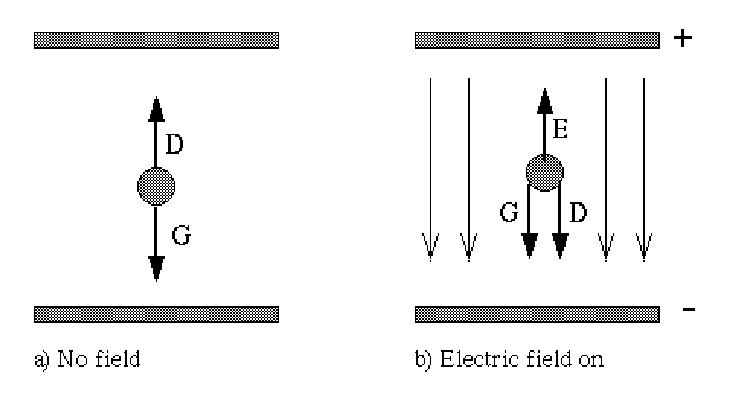
\epsfig{file=Introduction/oil_droplet.eps, height=5cm}
  \caption{
    Forces on an oil-droplet in: \newline
    \hspace*{1.5cm}
           a) Free fall          \newline
    \hspace*{1.5cm}
	   b) Electric field     \newline
    (G=Gravitation, D=Drag, E=Electric force)
  }
  \label{oil_droplet}
\end{center}
\end{figure}

His results were systematically low by about 4\% due to inaccurate
knowledge of the coefficient of viscosity. \newline
The electron charge is -e,
where $e = 1.602 \cdot 10^{-19}C$. All free particles are observed to
have values of electric charge equal to an integer times the
fundamental charge e:

\begin{equation*}
  q=n e
\end{equation*}

where the integer $n=\dots,-1,0,1,\dots$ is the electric charge
\emph{quantum number}.

\subsection*{The Nucleus}

In 1912, Ernest Rutherford and his associates discovered that the
positive charge of the atom is concentrated in a \emph{nucleus}. The
charge of the $\alpha$ particle, discovered by Becquerel, was
determined to be $2e$, and the mass of the $\alpha$ particle was
determined to be about four times the mass of the hydrogen
atom. \newline
A new particle with zero electric charge was discovered by bombarding
beryllium atoms with $\alpha$ particles. James Chadwick showed that
the new particle, the \emph{neutron}, had mass nearly equal to that of
the \emph{proton}.

\subsection*{The Bohr Model of the Atom}

In 1913, Niels Bohr made the first qunatitatively successful model of
the atom. Inspired by the work of Rutherford, Bohr made a planetary
model of the atom; with electrons moving in circular orbits about the
nucleus. This model may seem quite simple in retrospect, but for the
time it was a great advancement of science. In addition to the
classical circular orbits, the second part of Bohr's atomic model
contains a bold hypothesis of new physics. The new physics recognizes
that \emph{angular momentum} is \emph{quantized}; it can take only
certain values:

\begin{equation*}
  L = mvr = n \hbar
\end{equation*}

where $n$ is a positive integer. Solving the energy equations result
in orbits of radius:

\begin{equation*}
  r_n = \frac{n^2\hbar^2}{mke^2}
\end{equation*}

where the \emph{Bohr radius}

\begin{equation*}
  a_0 \equiv r_1 = \frac{\hbar^2}{mke^2} \approx 0.053 nm
\end{equation*}

is in the correct order of magnitude for the size of the atom!

{\bf Planc }


\part{Theory}
%\newtheorem{postulate}{Postulate}[chapter]
\newcommand{\tr}[1]{\text{Tr}\left(#1\right)}

\part{Theory}
\label{part:theory}

\chapter{Quantum Mechanics}
\label{ch:qm}
Quantum mechanics governs the behaviour of everything. In fact, both the tool we will be using for the thesis, quantum computing, and the problem we are trying to solve, the ground state energy of a Hamiltonian, are tightly connected to the principles of quantum mechanics. It is therefore important that we devote this chapter to the theory of quantum mechanics. We start by introducing notations, followed by postulates and key definitions and theorems, including the variational principle and basic many-body physics. We will follow the textbook \textit{Quantum Mechanics}~\cite{schiff1968} in the formulation.
\section*{Symbols and Notations}
\label{sec:notations}

The notations defined in Table~\ref{tab:notations} are used throughout this thesis. Table~\ref{tab:notations} includes symbols for many essential concepts for the topic of quantum computing. Note that the hat on an operator $ \hat A $ is often omitted for simplicity when there is no ambiguity. 
\begin{table}[ht]
	\centering
	\caption{Notations}
	\label{tab:notations}

	\begin{tabular}{ll}
		\toprule
		Notation & Meaning \\
		\midrule
		$ \ket{\psi} $ & State vector, ket \\
		$ \bra{\psi} $ & Dual vector of $ \ket{\psi} $, bra \\
		$ \braket{\psi|\phi} $ & Inner product of $ \ket{\psi} $ and $ \ket{\phi} $ \\
		$ \ket{\psi}\bra{\phi} $ & Outer product of $ \ket{\psi} $ and $ \ket{\phi} $ \\
		$ \hat A$ & operator A \\
		$ \hat I $ & Identity operator \\
		$ \braket{\psi|\hat A|\psi} $ & Expectation value of $ \hat A $ in $ \ket{\psi} $ \\
		$ [\hat A, \hat B] $ & Commutator of $ \hat A $ and $ \hat B $ \\
		$ \{\hat A, \hat B\} $ & Anti-commutator of $ \hat A $ and $ \hat B $ \\
		$ \hat A^\dagger $ & Hermitian conjugate of $ \hat A $ \\
		$ \tr{\hat A} $ & Trace of $ \hat A $ \\
		%$ Tr_A(\hat A) $ & Partial trace of $ \hat A $ over $ \mathcal{H}_A $ \\
		$ A \otimes B $ & Tensor product of $ \hat A $ and $ \hat B $ \\
		$ X,Y,Z $ & Pauli $ \sigma_x, \sigma_y \text{ and } \sigma_z $ matrices \\
            $ \mathcal{H}$ Hilbert space \\
	\bottomrule	
	\end{tabular}
\end{table}

\section{Postulates}
\label{sec:posulates}

The postulates of quantum mechanics are the basic assumptions and the foundation of the theory, every other theorem in quantum mechanics follows as a consequence. They are the assumptions that the theory is built upon. The postulates are listed below:


\begin{postulate}{}{qm1}
	The state of a quantum system is described by a ket vector $ \ket{\psi} $ in a Hilbert space $ \mathcal{H} $.
\end{postulate}
This is the \textbf{state postulate}, it states that the state vector $\ket{\psi}$ contains all the information about the system

\begin{postulate}{}{qm2}
	Every observable quantity is associated with a Hermitian operator $ \hat A $ in $ \mathcal{H} $. $\braket{A} = \braket{\Psi|A|\Psi}$ is the expectation value of $ \hat A $ in the state $ \ket{\Psi} $. The only possible result of a measurement of an observable $ \hat A $ is one of the eigenvalues of $ \hat A $.
\end{postulate}
As we will discuss later in Subsection~\ref{sub:hermitian}, the eigenvalues of Hermitian operators are real, which is an important consequence as the measurement results of any oberservable has to be real.
\begin{postulate}{}{qm3}
	The time evolution of a wave function is governed by the Schr{\"o}dinger equation:
	\begin{equation}
		i\hbar\frac{\partial}{\partial t}\ket{\Psi(t)} = \hat H\ket{\Psi(t)}.
	\end{equation}
\end{postulate}
This is the \textbf{evolution postulate}, it describes how the quantum system changes over time if undisturbed, through e.g. measurement.


\begin{postulate}{}{pos:qm4}
	The probability of measuring an observable $ \hat A $ in the state $ \ket{\Psi} $ is given by:
	\begin{equation}
		P(a) = \left | {\braket{\Psi|a}}^2 \right |,
	\end{equation}
	where $ \ket{a} $ is an eigenstate of $ \hat A $.
\end{postulate}
Opposite to Postulate~\ref{pos:qm3}, the \textbf{measurement postulate} describes the behaviour of a quantum system when disturbed.

\begin{postulate}{}{qm5}
	The eigenvectors of a Hermitian operator form a complete basis, which means that any state vector can be expressed as a linear combination of the eigenvectors:
	\begin{equation}
		\ket{\Psi} = \sum_{i} c_i \ket{\psi_i},
	\end{equation}
where $ \{ \psi_i \}  $ is a complete basis set. 
\end{postulate}

\section{The Schr{\"o}dinger Equation}

The Schr{\"o}dinger equation is the fundamental equation of quantum mechanics. It describes the time evolution of a quantum system without measurement. Since the norm of the state vector must be conserved, the time evolution operator in quantum mechanics therefore must be unitary. The Schr{\"o}dinger equation is given by:
\begin{equation}
	\label{eq:schrodinger}
i\hbar\frac{\partial}{\partial t}\ket{\Psi(t)} = \hat H\ket{\Psi(t)},
\end{equation}
where $ \hat H $ is the Hamiltonian operator of the system. 
The time independent Schr{\"o}dinger equation is given by:
\begin{equation}
	\label{eq:time_independent_schrodinger}
	\hat H\ket{\Psi} = E\ket{\Psi},
\end{equation}
where $ E $ is the energy of the system. The solution to the time independent Schr{\"o}dinger equation (TISE) is the eigenvalue of the Hamiltonian operator. The ground state energy problem which we will be solving using the VQE in Chapter~\ref{chap:results} is fundamentally the TISE.

\section{Special Types of Operators in Quantum Mechanics}
According to Postulate~\ref{pos:qm2}, every observable can be represented by a Hermitian operator. In this section, we will discuss the properties of operators and their representations.

\begin{theorem}{Spectral Theorem}{spectral}
If $ \hat A $ is a Hermitian operator in vector space $ V $, then there exists an orthonormal basis of $ V $ consists of eigenvector of $ \hat A $. Each eigenvalue of $ \hat A $ is real.  The spectral decomposition of a Hermitian operator $ \hat A $ is given by:
\begin{equation}
	\hat A = \sum_{i} a_i \ket{\psi_i}\bra{\psi_i},
\end{equation}
where $ a_i $ is the eigenvalue of $ \hat A $ and $ \ket{\psi_i} $ is the corresponding eigenvector.
\end{theorem}
Rewriting the operators in a different basis is extremely important in quantum computing, as we will see in Chapter~\ref{ch:qc}.

\subsection{Hermitian Operators}
\label{sub:hermitian}

\begin{definition}{Hermitian Operators}{hermitian}
An operator $ \hat A $ is Hermitian if it satisfies:
\begin{equation}
	\hat A = \hat A^\dagger,
\end{equation}
where $ \hat A^\dagger $ is the Hermitian conjugate of $ \hat A $. 

The Hermitian conjugate of an operator is defined as:
\begin{equation}
	\braket{\psi|\hat A^{\dagger} |\phi} = \braket{\phi|\hat A|\psi}^*.
\end{equation}

\end{definition}
Example of famous Hermitian operators include the Pauli matrices, $\sigma_x, \sigma_y$ and $\sigma_z$.


The eigenvalues of a Hermitian operator are real, as 
\begin{equation}
\begin{aligned}
	\braket{\psi|a|\psi}^* &= \braket{\psi|\hat A^{\dagger}|\psi} = \braket{\psi|\hat A|\psi} = \braket{\psi|a|\psi}, \\
					&\implies \braket{\psi|a|\psi} = a \braket{\psi|\psi}  \in \mathbb{R}, \\
					&\implies a \in \mathbb{R} \quad \quad \text{since} \braket{\psi|\psi} \in \mathbb{R},
\end{aligned}
\end{equation}
where $ a $ is an eigenvalue of $ \hat A $.
This ensures that all measurable quantities and expectation values are real.

\subsection{Unitary Operators}
\label{sub:unitary}
\begin{definition}{Unitary Operators}{unitary}
	An operator $ \hat U $ is unitary if it satisfies:
	\begin{equation}
		\hat U^\dagger \hat U = \hat U \hat U^\dagger = \hat I.
	\end{equation}
\end{definition}


This is an important property for quantum gates to have, as it ensures that the norm and orthogonality of the state vector are preserved . \\
Given an initial state $ \ket{\psi(0)} $ and any operator $ \hat U $. The evolution is given by
\[ \hat U \ket{\psi(0)} = \ket{\psi(t)}.  \]
By requiring the norm of the state vector to be preserved, we have
\[ \braket{\psi(0)|\psi(0)} = \braket{\psi(t)|\psi(t)} = \braket{\psi(0)|U^{\dagger}U|\psi(0)}, \] 
\[ \implies U^{\dagger}U = \hat I, \] 
hence $ U $ is unitary.

\subsection{Commutators and Anticommutators}
Operators in general do not commute. Two commuting operators have the same eigenvectors and can be measured simultaneously. Finding commuting terms in the Hamiltonian could save the number of measurements in the context of quantum computing. The anti-commutation relation for fermions are extremely important in quantum computing and that is the reason why mappings like the Jordan-Wigner transformation must respect the anti-commutation relation for fermionic operators.
\begin{definition}{Commutator}{commutator}
	The commutator of two operators $ \hat A $ and $ \hat B $ is defined as:
	\begin{equation}
		[\hat A, \hat B] = \hat A \hat B - \hat B \hat A.
	\end{equation}
		The anticommutator of two operators $ \hat A $ and $ \hat B $ is defined as:
	
	\begin{equation}
		\{\hat A, \hat B\} = \hat A \hat B + \hat B \hat A.
	\end{equation}
\end{definition}

Important commutation relations are given in Appendix~\ref{appsec:commutation_relations}.

\section{Density Matrix}
\label{sec:density_matrix}
The density operator is useful to describe a mixed state, which contain classical uncertainties that cannot be described using superposition. In finite dimensional space, the density operator can be written as a matrix and is therefore often called the \textit{density matrix}.  
\begin{definition}{Density Matrix}{density_matrix}
	The density matrix $ \rho $ is defined as:
	\begin{equation}
		\rho = \sum_{i} p_i \ket{\psi_i}\bra{\psi_i},
	\end{equation}
	where $ p_i $ is the probability of the state $ \ket{\psi_i} $.
\end{definition}

The expectation value of an observable $ \hat A $ in a classical ensemble of states described by the density matrix $ \rho $ is given by:
\begin{equation}
\begin{aligned}
	\braket{A} &= \sum_j P_j \braket{\psi_j|A|\psi_j}, \\
		   &= \sum_j P_j \braket{\psi_j|\sum_k |k} \braket{k|\hat A|\psi_j}, \\
		   &= \sum_{j,k} P_j \braket{\psi_j|k} \braket{k|\hat A|\psi_j}, \\
		   &= \sum_{j,k} P_j \braket{k|\hat A|\psi_j} \braket{\psi_j|k}, \\
		   &= \tr{\hat A \rho}.
\end{aligned}
\end{equation}

For a pure state $ \ket{\psi} $, the density matrix is the projector:
\begin{equation}
	\rho = \ket{\psi}\bra{\psi}.
\end{equation}

\section{Entanglement}
\label{sec:entanglement}
Entanglement is a purely quantum mechanical phenomenon where two or more different quantum states, (particles or otherwise), become correlated where measurements to one state can determine the other(s) state(s) instantaneously. This is one of the many reasons why quantum computers might be better than classical computers.
For two states $ \ket{\psi}  $ and $ \ket{\phi} $ in two Hilbert spaces $ \mathcal{H}_1 $ and $ \mathcal{H}_2 $ with basis $ \{\ket{u_j} \} $ and $ \{\ket{w_j} \} $  respectively, the tensor product $ \ket{\psi} \otimes \ket{\phi} $ is a state in the Hilbert space $ \mathcal{H}_1 \otimes \mathcal{H}_2 $. This is called a \textit{product state} and if
\[ \ket{\psi} = \sum_j d_j \ket{u_j},\] and \[ \ket{\phi} = \sum_k f_k \ket{w_k},\] 
then
\[ \ket{\psi} \otimes \ket{\phi} = \sum_{j,k} d_j f_k \ket{u_j} \otimes \ket{w_k}.\]
An arbitrary state $ \ket{\Psi} $ in the combined Hilbert space can be written as:
\[ \ket{\Psi} = \sum_{j,k} c_{jk} \ket{u_j} \otimes \ket{u_k}, \] 
with coefficients $ c_{jk} $.
A product state has separable coefficients. If the coefficients $ c_{jk} $  are not separable, the state $ \ket{\Psi} $ is called an entangled state. 

\section{the Variational Principle}
\label{sec:variational_principle}
The variational method provides an upper bound on the ground state energy levels of a system. It is given by
\begin{equation}
	\label{eq:variational_principle}
	E_0 \leq \bra{\psi(\vec{\theta)}} \hat H \ket{\psi(\vec{\theta)}}.
\end{equation}
Note that the equality is only true when $\ket{\psi}$ is the ground state.
It consists of two steps:
\begin{enumerate}
	\item Choose an ansatz $\ket{\psi(\vec{\theta_0})}$ for the ground state.
	\item Optimise the parameter $\vec{\theta}$ of the ansatz to minimise the energy.
\end{enumerate}
The variational principle allows us to find the ground state energy using iterative methods which is the key principle behind the VQE. 



\section{Many-Body Physics}
\label{sec:many_body_physics}
Most problems we will attempt to solve in this thesis are fundamentally many-body problems.
In this section, we will discuss the many-body basis, indistinguishability and the second quantization formalism.

\subsection{Many-Body Basis}
\label{sub:many_body_basis}
If the single particle state is represented by $ \{ \ket{\phi_i} \} $, a single particle state $ \ket{\psi}  $  can be represented by
\begin{equation}
	\ket{\psi_{\text{1-particle}}}  = \sum_{j} c_j \ket{\phi_{j}}.
\end{equation}
Then the $ N $ identical particle state can be written as a tensor product of the single particle basis:
\begin{equation}
	\label{eq:many_body_state}
	\ket{\psi_{\text{N-particle}}} = \sum_{j_1, j_2, \ldots, j_N} c_{j_1, j_2, \ldots, j_N} \ket{\phi_{j_1}} \otimes \ket{\phi_{j_2}} \otimes \cdots \otimes \ket{\phi_{j_N}}.
\end{equation}

\subsection{indistinguishability}
\label{sub:indistinguishability}
Fundamental particles are indistinguishable. This means that the state of a system is invariant under the exchange of two particles. If $ \hat P_{ij} $ is the particle exchange operator which exchanges state of particle $ i $ and particle $ j $,
\begin{equation}
	\label{eq:indistinguishability}
	\hat P_{ij} \ket{\psi(0,\ldots,i,\ldots,j,\ldots)} = e^{i\phi}\ket{\psi(0,\ldots,j,\ldots,i,\ldots)}. \\
\end{equation}
Since the physics is invariant under the exchange of two particles, the state can only differ by a global phase. Applying the particle exchange operator again must give the exact state that we have started with.
\begin{equation}	
	\hat P_{ij}^2 \ket{\psi(0,\ldots,i,\ldots,j,\ldots)} = e^{2i\phi}\ket{\psi(0,\ldots,i,\ldots,j,\ldots)} = \ket{\psi(0,\ldots,i,\ldots,j,\ldots)} 
\end{equation}
This implies that $ e^{2i\phi} = 1 $, hence $ e^{i\phi} = \pm 1$, which means that the state is either symmetric or antisymmetric under the exchange of two particles. 

The principle of indistinguishability results in that the actual space for the both fermions and bosons are smaller than the tensor product of the single particle Hilbert space.


\subsection{Occupation Number (Second Quantisation) Notation}
\label{sub:occupation_number_notation}

Because of the indistinguishability discussed in Section~\ref{sub:indistinguishability}, the coefficients $ \{ c_{j_{n}} \}  $ in Equation~\eqref{eq:many_body_state} are not independent and not all elements of the combined Hilbert space are physical states. The occupation number notation provides a different way to represent the many-body state, also called second quantisation formalism. Since the fundamental particles are either symmetric or antisymmetric under exchange of particles, one could simply the number of particles in a given state, hence the occupation number notation. In the occupation number notation, Equation~\eqref{eq:many_body_state}
becomes:
\begin{equation}
	\label{eq:occupation_number_notation}
	\ket{\psi_{\text{N-particles}}} = \sum_{n_1, n_2, \ldots, n_N} c_{n_1, n_2, \ldots, n_N} \ket{n_1, n_2, \ldots, n_N}.
\end{equation}
Note that the coefficients $ \{ c_n \}  $ are now independent and normalised. \\
While Equation~\eqref{eq:occupation_number_notation} looks similar to Equation~\eqref{eq:many_body_state}, they have very different physical interpretations. The state $ \ket{\phi_{j_n}} $ is a state of the $ N $th particle and the state $ \ket{n_N} $ gives the number of particles in the single particles state $ \ket{\phi_N}  $.

\subsubsection{Fock Space}
\label{sub:fock_space}
The occupation number notation introduces the possibility of having different numbers of the particles in a state, say
\[ \ket{\psi} = \ket{1,1,0} + \ket{1,0,0}, \]
where we assume for $\ket{1}$ means a state is occupied and $\ket{0}$ otherwise. The first part of the equation is a state with $2$ particles and the second part of the state has $1$ particle. This is allowed with the occupation number notation.
The space of all possible number of particles is called the Fock space.
The Fock space is the direct sum of the Hilbert space of all possible number of particles up to $ N $ . The Fock space is given by:
\begin{equation}
	F_v(\mathbb{H}) = \bigoplus_{n=0}^{N} \hat S_v \mathbb{H}^{\otimes n}.
\end{equation}
where $ \hat S_v $ is the symmetrisation operator for bosons and the antisymmetrisation operator for fermions, and$ \bigoplus $is summation over spaces. 

\subsubsection{Operators in Second Quantisation}
\label{sub:second_quantization}
The creation operator is defined as:
\begin{definition}{Creation Operator}{fermionic_creation}
	\begin{equation}
		\hat a_i^\dagger \ket{0} \equiv \ket{i},
	\end{equation}	
\end{definition}
where $ \ket{0} $ is the vacuum state and $ \ket{i} $ is the state with one particle in the $ i $th single particle state.
The hermitian conjugate of the creation operator, $ \hat a_i $ is the annihilation operator since
\begin{equation}
	\hat a_i \ket{i} = \ket{0}.
\end{equation}
The number operator is given by:
\begin{equation}
	\label{eq:number_operator}
	\hat n_i = \hat a_i^\dagger \hat a_i.
\end{equation}

An Hamiltonian operator $ \hat H $ with one-body and two-body interactions in the first quantisation formalism can be written in the second quantisation formalism as:
\begin{equation}
	\begin{aligned}
		\hat H &= \sum_{p} \hat T_p + \sum_{p \neq q} \hat V_{pq}, \\
			&= \sum_{i,j} h_{ij} \hat a_i^\dagger \hat a_j + \frac{1}{2}\sum_{i,j,k,l} v_{ijkl} \ \hat a_i^\dagger \hat a_j^\dagger \hat a_k \hat a_l,
	\end{aligned}
\end{equation}
where $h_ij$ and $v_ijkl$ are the one- and two- body coefficients.


\subsection{Fermionic Operators}
\label{sub:fermionic}
The principle of indistinguishability states that under the exchange of particles, the total many-body wavefunction be either symmetric or anti-symmetric, as we have shown in Subsection~\ref{sub:indistinguishability}. The Pauli exclusion principle states the many-body states for fermions are anti-symmetric under the exchange of particles, and for boson are symmetric. The obey the anti-commutation relation given in Appendix~\ref{appsec:commutation_relations}.

\subsection{Slater Determinant}
\label{sub:slater_determinant}
The Slater determinant is a way to antisymmetrise the many-body wave function. It is given by:
\begin{equation}
	\ket{\psi} = \frac{1}{\sqrt{N!}} \begin{vmatrix}
		\psi_1(1) & \psi_2(1) & \ldots & \psi_N(1) \\
		\psi_1(2) & \psi_2(2) & \ldots & \psi_N(2) \\
		\vdots & \vdots & \ddots & \vdots \\
		\psi_1(N) & \psi_2(N) & \ldots & \psi_N(N)
        \end{vmatrix}.
\end{equation}
where $ \psi_i(j) $ is the $ i $th single particle state with the $ j $th particle. 



\chapter{Many-body theory}
\label{ch:manybody}
It is often insufficient to be able to calculate properties in systems with only one particle.
One would for example be restricted to only hydrogen, if studying atoms.
Methods for many-particle systems have thus been developed, often theoretically exact, but in practice we must rely on computer programs having a truncation affecting the accuracy of the results.
Different types of approximations, or many-body methods, exist, where widely used techniques are; full configuration interaction, many-body perturbation theory, Hartree-Fock theory, Monte-Carlo methods and coupled-cluster theory.
%MHJ forandra litt her
Even though we will focus mainly on the coupled-cluster approach, the concepts from this chapter are shared by several many-body methods based on wave functions constructed using a single-particle basis.


\section{The non-interacting case}
The natural starting point for many-body theory is to deal with non-interacting particles.
In this case the Schrödinger equation holds the same form now as it did for one particle in eq. \eqref{eq:qm:schrodingerbraket}.
Assuming a time-independent Hamiltonian,
\begin{equation}
\hat{H} = \sum_k \hat{h}_k =  \sum_k \hat{t}_k  + \sum_k \hat{v}_k ,
\end{equation}
with $\hat{t}_k$ and $\hat{v}_k$ being the operators for kinetic and potential energy for particle $k$, the energy is constant in time and we only need to solve the time-independent Schrödinger equation.
Since the particles are not interacting, this equation is separable, and we assume a total wave function, $|\Psi^{(\lambda)} \rangle$, being a product of different single-particle spin orbitals $|\psi_k^{(\lambda)}\rangle$, with a total energy $E^{(\lambda)}=\sum_k E_k^{(\lambda)}$,
\begin{equation}
\hat{H}|\Psi^{(\lambda)} \rangle = 
\left(\sum_k \hat{h}_k\right) \left(|\psi_1^{(\lambda)}\rangle \otimes |\psi_2^{(\lambda)}\rangle 
\cdots \otimes |\psi_N^{(\lambda)}\rangle \right)
=  \sum_k E_k^{(\lambda)} |\Psi^{(\lambda)} \rangle .
\end{equation}
Here $E_k^{(\lambda)}$ is the energy of particle $k$, satisfying the single-particle eigenvalue equation,
\begin{equation}
\label{eq:manybody:nonInter}
\hat{h}_k |\psi_k^{(\lambda)} \rangle = E_k^{(\lambda)} |\psi_k^{(\lambda)} \rangle .
\end{equation}
It is important to note how the subscript refers to the different particles, whereas the superscript denotes different eigenstates inside a spectrum of energies.

Electrons are, although it complicates our calculations, interacting through the coulomb interaction. 
%MHJ retting
For this reason we keep this simple separable calculation in memory when we move on to interacting 
many-body systems, where correlations play an important  as corrections to the non-interacting reference energy.


\section{Indistinguishable and identical particles}
An important aspect when considering systems with more than one particle is that electrons are identical and indistinguishable particles.
In quantum mechanics it makes no sense talking about different particles, they are truly identical and impossible to track one at a time.
As a consequence of this, interchanging the coordinates of two particles should not alter the probability distribution, i.e.
\begin{equation}
\label{eq:manybody:interchange}
| \Psi |^2
=
|\hat{P}_{ij} \Psi |^2 .
\end{equation}
This compact notation is due to the introduction of the permutation operator $\hat{P}_{ij}$, which interchanges particles $i$ and $j$. Equation~\eqref{eq:manybody:interchange} holds only if
\begin{equation}
\hat{P}_{ij} = \pm 1 ,
\end{equation}
where particles with a symmetric wave function, that is $\hat{P}_{ij} = 1$, are called bosons, while particles having an antisymmetric wave function, $\hat{P}_{ij} = -1$, are called fermions.

\paragraph*{}
Since electrons are fermions we need to construct wave functions that are antisymmetric.
The simple product of single-particle wave functions 
we assumed in the non-interacting case is thus not correct.
Antisymmetric wave functions are usually expressed as determinants, as proposed by John C. Slater, therefore called Slater determinants \cite{PhysRev.34.1293}.
Having a complete, orthonormal, single-particle basis where $N$ functions,  $\phi_{\alpha}, \phi_{\beta}, \cdots \phi_{\delta}$, are occupied by $N$ particles at different positions, $\vec{r_1}, \cdots , \vec{r_N}$, an $N$-particle wave function reads
\begin{equation}
\label{eq:manybody:slater}
\Phi_{\alpha,\beta,\cdots,\delta}(\vec{r_1},\cdots,\vec{r_N})
=
\frac{1}{\sqrt{N!}}
\left|
\begin{matrix}
\phi_{\alpha}(\vec{r_1}) & \phi_{\beta}(\vec{r_1}) & \cdots & \phi_{\delta}(\vec{r_1}) \\
\phi_{\alpha}(\vec{r_2}) & \phi_{\beta}(\vec{r_2}) & \cdots & \phi_{\delta}(\vec{r_2}) \\
\vdots                   & \vdots                  & \ddots & \vdots \\
\phi_{\alpha}(\vec{r_N}) & \phi_{\beta}(\vec{r_N}) & \cdots & \phi_{\delta}(\vec{r_N})\\
\end{matrix}
\right| .
\end{equation}
The notation here is of importance.
Up to now we have looked at the exact solution, denoted $\Psi$.
In this step the single particle basis $\phi$ can be any complete basis, and therefore $\Phi$ is in general not the exact solution.
The solution can however be expressed as a linear combination of slater determinants, 
\begin{equation}
|\Psi^{(\lambda)} \rangle = 
\sum_{\alpha,\beta,\cdots,\delta} C_{\alpha,\beta,\cdots,\delta}^{(\lambda)}
|\Phi_{\alpha,\beta,\cdots,\delta} \rangle ,
\end{equation}
due to the completeness of our basis functions.
Determinants have the property of being zero whenever two columns are equal.
This is a manifestation of the exclusion principle formulated by Wolfgang Pauli in 1925~\cite{springerlink:10.1007/BF02980631}, two fermions cannot share the same set of quantum numbers, 
for which he later received the Nobel prize for in 1945~\cite{nobelPauli}.
Including the two spin states available for each electron, no more than two electrons can share the same orbital.

\paragraph*{}
To incorporate interactions between the electrons, we add an extra term, $\hat{v}_{kl}$, to $\hat{H}$,
\begin{equation}
\label{eq:manybody:hamiltonnbody}
\hat{H} = \sum_k \hat{t}_k  + \sum_k \hat{v}_k + \frac{1}{2}\sum_{kl} \hat{v}_{kl} ,
\end{equation}
which is a two-body potential between electron $k$ and $l$, and the
factor of $\frac{1}{2}$ comes from the fact that all contributions are counted
twice, assuming $\hat{v}_{kl} = \hat{v}_{lk}$.
In the case of electron structures, these terms are simply all pairs of Coulomb interactions.
It is possible to continue this, by adding three-, four-, up to N-body forces.
Three-body forces are often needed in nuclear physics, but the two-body nature of the coulomb interaction limits our calculations to only two.




\section{Second quantization}
Limiting ourself to systems of electrons only, we recall the antisymmetric Slater determinant, eq.~\eqref{eq:manybody:slater}, and assuming orthonormal single-particle states,
\begin{equation}
\label{eq:manybody:orthonormalsp}
\langle \phi_r | \phi_s \rangle = \delta_{rs} ,
\end{equation}
we fill the determinant with the $N$ lowest lying states.
This is called the reference state, or ground state, having all $N$ particles in states with the lowest possible energies, still obeying the exclusion principle.
From now on, all single-particle states within the reference determinant will
be labeled $i,j,...$, whereas states with higher energies are labeled $a,b,...$~.
The border between states within the determinant and higher states is called the Fermi level.
When referring to states without knowing whether they are above or below the Fermi level, we will label them $p,q,...$~.
In this representation, the ground state can be written in the occupancy notation,
\begin{equation}
| \Phi \rangle = | ijkl... \rangle .
\end{equation}


\paragraph*{}
We will now introduce creation and annihilation operators, similar to the ladder operators in section~\ref{sec:qm:ladder}.
Instead of raising/lowering the energy of one electron, these operators add or remove one electron from the Slater determinant.
Denoting an empty determinant as `$|\rangle$', we can fill it to the reference state by adding one electron at a time using creation operators,
\begin{equation}
|\Phi \rangle = \hat{i}^{\dagger}\hat{j}^{\dagger}\hat{k}^{\dagger} \cdots |\rangle .
\end{equation}
This ground state is sometimes written as $| 0 \rangle$ for simplicity.
It is also possible to remove one electron by the annihilation operator, e.g.
\begin{equation}
\hat{j} | \Phi \rangle = 
\hat{j} | ijk\cdots \rangle = 
- \hat{j} | jik\cdots \rangle =
- | ik\cdots \rangle .
\end{equation}
The minus sign here comes from the fact that these operators only alter the left-most state, and being antisymmetric one needs to multiply a factor of $-1$ for each permutation it takes to bring $j$ to the left side of the determinant.

It should not be allowed to annihilate an electron that is not present in the determinant, neither create an already present one.
With this in mind, it is clear that the following two statements must be true;
\begin{equation}
\label{eq:manybody:particlehole}
\begin{split}
\hat{p}^{\dagger} |\Phi \rangle &=
\left\lbrace
\begin{matrix}
|\Phi^{p} \rangle & \textrm{ if } p \in a,b,c,\cdots \\
0	                & \textrm{ if } p \in i,j,k,\cdots \\
\end{matrix}
\right. 
\\
\hat{p} |\Phi \rangle &=
\left\lbrace
\begin{matrix}
0                   & \textrm{ if } p \in a,b,c,\cdots \\
|\Phi_p \rangle     & \textrm{ if } p \in i,j,k,\cdots  \\
\end{matrix}
\right. 
\end{split}
\end{equation}
where $| \Phi_p \rangle$ means the reference state without $p$, and $| \Phi^p \rangle$ means the reference state with $p$ added.
In the particle-hole formalism everything is relative to the reference, where
an added electron is called a particle and a removed one referred to as a hole.
Generalizing this one can have multiple particles and holes. 
To prevent from creating a $0$-determinant, the hole states must be in $i,j,...$, and the particle states in $a,b,...$~.
An example could be
\begin{equation}
|\Phi_{ijk}^{ab} \rangle =
\hat{a}^{\dagger} \hat{b}^{\dagger} \hat{k} \hat{j} \hat{i} |\Phi \rangle .
\end{equation}
Having two particles and three holes, we call this a 2p-3h excitation.


\paragraph*{}
Because of the orthonormal single particle basis~(\ref{eq:manybody:orthonormalsp}), the determinants will be orthonormal too.
To be consistent, we define the empty vacuum state to be normalized as well,
\begin{equation}
\langle | \rangle = 1 .
\end{equation}
We see the importance of this when using the fact that creation and annihilation operators are each others adjoint,
\begin{equation}
\langle \Phi | \Phi \rangle = 
\left( \langle | \cdots \hat{j} \hat{i} \right) \left( \hat{i}^{\dagger} \hat{j}^{\dagger} \cdots | \rangle \right) =
 \langle | \left(  \cdots \hat{j} \hat{i}\hat{i}^{\dagger} \hat{j}^{\dagger} \cdots | \rangle \right)  .
\end{equation}
Since we first add $i,j,...$ to the vacuum before we remove the same particles, we end out with a vacuum state again,
\begin{equation}
 \langle | \left(  \cdots \hat{j} \hat{i}\hat{i}^{\dagger} \hat{j}^{\dagger} \cdots | \rangle \right) = 
 \langle | \rangle = 1 .
\end{equation}

\paragraph*{}
More rigorously, one may calculate the above using the  anti-commutation rules. 
Similar to the commutator, the anti-commutator is defined as 
\begin{equation}
[\hat{A},\hat{B}]_+ = \hat{A} \hat{B} + \hat{B} \hat{A} .
\end{equation}
We will start out with the annihilation operators by considering 
\begin{equation}
\begin{split}
\hat{p}\hat{q} | qpij\cdots \rangle &= |ij\cdots \rangle
\\
\hat{q}\hat{p} | qpij\cdots \rangle &= - \hat{q}\hat{p} | pqij\cdots \rangle = - | ij\cdots \rangle .
\end{split}
\end{equation}
One permutation is required for $\hat{q}\hat{p}$ since the operators only can act on the leftmost particle.
If neither $p$ nor $q$ is in the determinant then both of the expressions return zero.
In all cases the anti-commutator should be zero, thus
\begin{equation}
[\hat{p},\hat{q}]_+ = 0 .
\end{equation}
Considering two creation operators using the same procedure, we find that
$\hat{p}^{\dagger} \hat{q}^{\dagger} = - \hat{q}^{\dagger} \hat{p}^{\dagger}$
if neither $p$ nor $q$ is present in the determinant. If at least one of the
two is already present we get zero. Again the anti-commutator is zero, 
\begin{equation}
[\hat{p}^{\dagger},\hat{q}^{\dagger}]_+ = 0 .
\end{equation}
The last step is to look at one creation, and one annihilation operator.
If these two represent two different states ($p \neq q$), we have
\begin{equation}
\begin{split}
\hat{p}^{\dagger} \hat{q} |q ij\cdots \rangle &= |pij\cdots \rangle
\\
\hat{q} \hat{p}^{\dagger} |q ij\cdots \rangle &= 
\hat{q} |pqij\cdots \rangle = - |pij\cdots \rangle .
\end{split}
\end{equation}
With $q$ missing, or $p$ already present in the determinant the anti-commutator is zero, leading to 
\begin{equation}
[\hat{p}^{\dagger},\hat{q}]_+ = 0 \hspace{3mm}\textrm{ if }\hspace{1mm} p \neq q .
\end{equation}
If $p = q$, we need to investigate both when $p$ is already present and not,
\begin{equation}
\begin{split}
\hat{p} \hat{p}^{\dagger} |p ij\cdots \rangle &= 0 \\
\hat{p}^{\dagger} \hat{p} |p ij\cdots \rangle &= |pij\cdots \rangle \\
\hat{p} \hat{p}^{\dagger} |ij\cdots \rangle &= |ij\cdots \rangle \\
\hat{p}^{\dagger} \hat{p} |ij\cdots \rangle &= 0  ,
\end{split}
\end{equation}
which leads to the relation
\begin{equation}
[\hat{p}^{\dagger}, \hat{p}]_+ = 1 .
\end{equation}
All together we summarize to,
\begin{equation}
\label{eq:manybody:anticommutators}
\begin{split}
[\hat{p},\hat{q}]_+ &= 0 \\
[\hat{p}^{\dagger},\hat{q}^{\dagger}]_+ &= 0 \\
[\hat{p}^{\dagger},\hat{q}]_+ &= \delta_{pq} .
\end{split}
\end{equation}

Using the tools that the anti-commutators present, we could once again look at the normalized inner product
\begin{equation}
\langle i | i \rangle = \langle | \hat{i}\hat{i}^{\dagger} | \rangle
= \langle | -\hat{i}^{\dagger} \hat{i} + 1 | \rangle
= \langle | -\hat{i}^{\dagger} \hat{i} | \rangle + \langle | \rangle
= \langle | \rangle = 1 .
\end{equation}
The trick here was to switch place for $\hat{i}$ and $\hat{i}^{\dagger}$ by using the anti-commutation relation, and in the end reason that $\hat{i}|\rangle$ must be zero. 
For a general (wider) string of operators the same can be applied, but it is tedious, and better methods exist.



\subsection{Operators}
\label{sec:manybody:operators}
Suppose we rewrite the Hamiltonian from eq.~\eqref{eq:manybody:hamiltonnbody} as a sum of two terms, $\hat{H}^{(0)}$ and $\hat{H}^{(1)}$, where the first term contains all one-body terms and the second incorporates only the two body potential between electrons,
\begin{equation}
\begin{split}
\hat{H}^{(0)} &= \sum_{k=0}^N \left( \hat{t}_k + \hat{v}_k \right)
= \sum_{k=0}^N \hat{h}^{(0)}(x_k)
\\
\hat{H}^{(1)} &= \frac{1}{2} \sum_{kl}^N \hat{v}_{kl} (x_k, x_l) .
\end{split}
\end{equation}
Introducing atomic units, that is setting $\hbar = m_{e} = e = 1$, these operators can be expressed neatly as
\begin{equation}
\begin{split}
\hat{t}_k &= - \frac{1}{2} \nabla^2 \\ 
\hat{v}_{k} &= \frac{1}{2} \omega^2 x_k^2 \hspace{3mm}\textrm{ (for harmonic oscillator)} \\
\hat{v}_{kl} &= \frac{1}{|x_k - x_l|} \hspace{3mm}\textrm{ (for electrons)} .
\end{split}
\end{equation}


Before we express the operators in second quantization, using the creation and annihilation operators, we will define the number operator, which counts the number of occupied states in a determinant, hence the number of particles,
\begin{equation}
\label{eq:manybody:numberoperator}
\hat{N} = \sum_p \hat{p}^{\dagger} \hat{p} .
\end{equation}
This is the first example of a second quantized operator, and the most striking is the unrestricted sum, with $p$ looping through all values in our basis. In principle, this sum runs over infinitely many single-particle states.
Extending this for the different parts of our Hamiltonian, the one-body operator becomes
\begin{equation}
\hat{H}^{(0)} = \sum_{pq} \langle p| \hat{h}^{(0)} |q\rangle \hat{p}^{\dagger} \hat{q},
\end{equation}
and the two-body operator reads
\begin{equation}
\label{eq:manybody:twobody}
\begin{split}
\hat{H}^{(1)} &= \frac{1}{2} \sum_{pqrs} \langle pq | \hat{v} | rs \rangle 
\hat{p}^{\dagger} \hat{q}^{\dagger} \hat{s}\hat{r} \\
&= \frac{1}{4} \sum_{pqrs} \langle pq ||rs \rangle \hat{p}^{\dagger}
\hat{q}^{\dagger} \hat{s} \hat{r} .
\end{split}
\end{equation}
A usual interpretation is that $\hat{H}^{(0)}$ excites one particle from $q$ into a state
$p$ with a probability of
\begin{equation}
\langle p| \hat{h}^{(0)} |q\rangle = \int \phi_p^{*}(x_1) \hat{h}^{(0)}(x_1)
\phi_q(x_1) dx_1 ,
\end{equation}
whereas the two-body operator excites two particles from the states $r$ and $s$ into
$p$ and $q$, with a probability amplitude of
\begin{equation}
\langle pq | \hat{v} | rs \rangle =
\int \int \phi_p^{*}(x_1)\phi_q^{*}(x_2) \hat{v}(x_1,x_2) \phi_r(x_1)
\phi_s(x_2) dx_1 dx_2 .
\end{equation}
In the two-body case the probability amplitude is written directly as an integral,
without taking $|rs\rangle$ as an antisymmetric determinant.
To account for this, one often use the antisymmetric element instead, defined as
\begin{equation}
\label{eq:manybody:v_elem}
\langle pq | | rs \rangle = \langle pq |v| rs \rangle - \langle pq |v| sr
\rangle .
\end{equation}
This expression will still not account for the factor $\frac{1}{\sqrt{2}}$ in
front of a slater determinant, which is why we need a factor $\frac{1}{4}$ when
using this in equation~\eqref{eq:manybody:twobody}.

\paragraph*{}
With these forms of our operators, we can calculate expectation values in a
general way between two determinants.
For instance $\langle ij|\hat{V}|kl \rangle$ can be calculated using anticommutators,
\begin{equation}
\label{eq:manybody:anticomEval}
\begin{split}
\langle ij|\hat{V}|kl \rangle &= 
\frac{1}{4} \sum_{pqrs} \langle pq||rs \rangle 
\langle | \hat{j}\hat{i} 
\hat{p}^{\dagger} \hat{q}^{\dagger} \hat{s} \hat{r}
\hat{k}^{\dagger} \hat{l}^{\dagger} | \rangle 
= 
\frac{1}{4} \sum_{pqrs} \langle pq||rs \rangle 
\langle | \hat{j}
\left(\delta_{ip} -  \hat{p}^{\dagger} \hat{i} \right)
\hat{q}^{\dagger} \hat{s} \hat{r}
\hat{k}^{\dagger} \hat{l}^{\dagger} | \rangle \\
%
&= 
\frac{1}{4} \sum_{pqrs} \langle pq||rs \rangle \langle |
 \delta_{ip}  \hat{j}\hat{q}^{\dagger} \hat{s} \hat{r}\hat{k}^{\dagger}\hat{l}^{\dagger} -
\hat{j}  \hat{p}^{\dagger} \hat{i} \hat{q}^{\dagger} \hat{s} \hat{r}\hat{k}^{\dagger} \hat{l}^{\dagger} 
| \rangle  \\
&= 
\frac{1}{4} \sum_{pqrs} \langle pq||rs \rangle \langle |
\delta_{ip} \delta_{jq} \hat{s} \hat{r}\hat{k}^{\dagger}\hat{l}^{\dagger} +
\delta_{ip} \hat{q}^{\dagger}  \hat{j}\hat{s} \hat{r}\hat{k}^{\dagger}\hat{l}^{\dagger} -
\hat{j}  \hat{p}^{\dagger} \hat{i} \hat{q}^{\dagger} \hat{s} \hat{r}\hat{k}^{\dagger} \hat{l}^{\dagger} 
| \rangle .
\end{split}
\end{equation}
The second term on the last line of eq.~\eqref{eq:manybody:anticomEval} has $\hat{q}^{\dagger}$ as the leftmost operator.
Acting from the left on a vacuum bra state, this leads to zero.
The philosophy is to continue this process, moving creation operators
to the left in all terms.
The only contributing terms will then have Kronecker deltas only, i.e.
\begin{equation}
\label{eq:manybody:evaluationanticom}
\begin{split}
\langle ij|\hat{V}|kl \rangle &= 
\frac{1}{4} \sum_{pqrs} \langle pq||rs \rangle \langle |
\delta_{ip} \delta_{jq} \delta_{rk} \delta_{sl}
- \delta_{ip} \delta_{jq} \delta_{sk} \delta_{rl}
+ \delta_{jp} \delta_{iq} \delta_{sk} \delta_{rl}
- \delta_{jp} \delta_{iq} \delta_{rk} \delta_{sl}
|\rangle \\
&=
\frac{1}{4} \left[
 \langle ij||kl \rangle
-\langle ij||lk \rangle
+\langle ji||lk \rangle
-\langle ji||kl \rangle
\right]
=
\langle ij||kl \rangle .
\end{split}
\end{equation}
The last step here was to see that all terms are exactly the same, due to the
antisymmetric elements, where
\begin{equation}
 \langle ij||kl \rangle =
-\langle ij||lk \rangle =
\langle ji||lk \rangle =
-\langle ji||kl \rangle .
\end{equation}


\subsection{Wick's theorem}
Anticommutators, as seen in the previous section, are powerful, yet
tedious, constructs for calculation of expectation values.
Any state can be transformed into a string of operators acting on the vacuum,
which we can transform further by anticommutators.
For strings of more operators one could automate this process, by using sympy~\cite{sympy}
or similar software, but for closed-form 
calculations, Wick's time-independent theorem allows for substantial  simplifications.

\paragraph*{}
Having a string of operators $\hat{A} \hat{B} \hat{C} ...$, we define the
normal-ordered product 
\begin{equation}
\left\lbrace  \hat{A} \hat{B} \hat{C} ...  \right\rbrace ,
\end{equation}
as a reordered product, with all creation operators moved to the left, and
annihilation operators to the right.
A phase phactor of $-1$ will arise whenever an odd number of permutations is
needed in the reordering.
Such a product is extremely usefull due to the fact that all expectation values
in vacuum yields zero.
Furthermore we define a contraction between two operators as the difference between the original
ordering and the normal ordering,
\begin{equation}
\contraction[1ex]{}{\hat{A}}{}{\hat{B}}
\hat{A}\hat{B}
=
\bcontraction[1ex]{}{\hat{A}}{}{\hat{B}}
\hat{A}\hat{B}
=
\hat{A}\hat{B} - \left\lbrace \hat{A}\hat{B} \right\rbrace .
\end{equation}
With this approach, four contractions are possible;
\begin{equation}
\label{eq:manybody:vacuumcontractions}
\begin{split}
\contraction[1ex]{}{\hat{p}}{}{\hat{q}}
\hat{p}\hat{q} &= \hat{p}\hat{q} - \hat{p}\hat{q} = 0 \\
%
\contraction[1ex]{}{\hat{p}}{}{\hat{q}^{\dagger}}
\hat{p}\hat{q}^{\dagger} &= \hat{p}\hat{q}^{\dagger} -(-\hat{q}^{\dagger}
\hat{p}) = \delta_{pq}\\
%
\contraction[1ex]{}{\hat{p}^{\dagger}}{}{\hat{q}}
\hat{p}^{\dagger}\hat{q} &= \hat{p}^{\dagger}\hat{q} - \hat{p}^{\dagger}\hat{q}
= 0\\
%
\contraction[1ex]{}{\hat{p}^{\dagger}}{}{\hat{q}^{\dagger}}
\hat{p}^{\dagger}\hat{q}^{\dagger} &= \hat{p}^{\dagger}\hat{q}^{\dagger} -
\hat{p}^{\dagger}\hat{q}^{\dagger} = 0  .
\end{split}
\end{equation}
If contractions occur within a normal product, a phase factor of $-1$ will
arise from each permutation that is needed to bring the contracted operators
besides each other.

Wick's theorem~\cite{PhysRev.80.268} states that any string of operators can be rewritten as a sum,
where the first term is the normal-ordered string.
The second term is a sum of all possible normal products with contractions between two operators only.
The next term is a sum of possible contractions between four operators, and so
on up to a sum of all possibilities where all operators are contracted.
The nice feature of this theorem is that all products with normal ordered
strings will not give a contribution when evaluated between vacuum states.
In this case only terms that are fully contracted will contribute.

If we have a product of two already normal-ordered operator strings, this is rewritten as the normal-ordered string off all operators plus all possible contractions between the first and the second string.
As an example we will return to the transition probability from
equation~\eqref{eq:manybody:evaluationanticom}, using Wick's theorem instead,
%THIS SIMPLE WICK LOOKS FISHY
\begin{equation}
\begin{split}
\label{eq:manybody:evaluationwick}
&\langle ij|\hat{V}|kl \rangle = 
\frac{1}{4} \sum_{pqrs} \langle pq||rs \rangle 
\langle | \hat{j}\hat{i} 
\hat{p}^{\dagger} \hat{q}^{\dagger} \hat{s} \hat{r}
\hat{k}^{\dagger} \hat{l}^{\dagger} | \rangle \\
%
&= 
\frac{1}{4} \sum_{pqrs} \langle pq||rs \rangle \langle | 
\contraction[1ex]{}{\hat{j}}{\hat{i}}{ \hat{p}}
\contraction[1.6ex]{\hat{j}}{\hat{i}}{\hat{p}^{\dagger}}{\hat{q}}
\hat{j}\hat{i} \hat{p}^{\dagger} \hat{q}^{\dagger} 
\contraction[1ex]{}{\hat{s}}{\hat{r}}{\hat{k}}
\contraction[1.6ex]{\hat{s}}{\hat{r}}{\hat{k}^{\dagger}}{\hat{l}}
\hat{s} \hat{r}\hat{k}^{\dagger} \hat{l}^{\dagger} 
+
\contraction[1ex]{}{\hat{j}}{\hat{i}}{ \hat{p}}
\contraction[1.6ex]{\hat{j}}{\hat{i}}{\hat{p}^{\dagger}}{\hat{q}}
\hat{j}\hat{i} \hat{p}^{\dagger} \hat{q}^{\dagger} 
\contraction[1ex]{\hat{s}}{\hat{r}}{}{\hat{k}}
\contraction[1.6ex]{}{\hat{s}}{\hat{r}\hat{k}^{\dagger}}{\hat{l}}
\hat{s} \hat{r}\hat{k}^{\dagger} \hat{l}^{\dagger} 
+
\contraction[1ex]{\hat{j}}{\hat{i}}{}{ \hat{p}}
\contraction[1.6ex]{}{\hat{j}}{\hat{i}\hat{p}^{\dagger}}{\hat{q}}
\hat{j}\hat{i} \hat{p}^{\dagger} \hat{q}^{\dagger} 
\contraction[1ex]{\hat{s}}{\hat{r}}{}{\hat{k}}
\contraction[1.6ex]{}{\hat{s}}{\hat{r}\hat{k}^{\dagger}}{\hat{l}}
\hat{s} \hat{r}\hat{k}^{\dagger} \hat{l}^{\dagger} 
+
\contraction[1ex]{\hat{j}}{\hat{i}}{}{ \hat{p}}
\contraction[1.6ex]{}{\hat{j}}{\hat{i}\hat{p}^{\dagger}}{\hat{q}}
\hat{j}\hat{i} \hat{p}^{\dagger} \hat{q}^{\dagger} 
\contraction[1ex]{}{\hat{s}}{\hat{r}}{\hat{k}}
\contraction[1.6ex]{\hat{s}}{\hat{r}}{\hat{k}^{\dagger}}{\hat{l}}
\hat{s} \hat{r}\hat{k}^{\dagger} \hat{l}^{\dagger} 
| \rangle \\
%
&= 
\frac{1}{4} \sum_{pqrs} \langle pq||rs \rangle \langle |
 \delta_{jp} \delta_{iq} \delta_{sk} \delta_{rl}
- \delta_{jp} \delta_{iq} \delta_{rk} \delta_{sl}
+ \delta_{ip} \delta_{jq} \delta_{rk} \delta_{sl}
- \delta_{ip} \delta_{jq} \delta_{sk} \delta_{rl}
|\rangle .
%
\end{split}
\end{equation}
This is not all fully contracted terms, but with a little reasoning it seems
clear that the other terms have at least one contraction that is equal to zero.
It is possible to count the number of crossing lines, instead of 
moving operators close to each other, to get the correct phase factor.
The number of crossings are $(2,1,0,1)$ in the four terms, leading to a minus
sign in the second and the last term, due to an odd number of crossings.
Comparing \eqref{eq:manybody:evaluationwick} with
%MHJ forandring
\eqref{eq:manybody:evaluationanticom}, we see that both yield the correct result, however,
using Wick's theorem simplifies considerably the algebra.


\paragraph*{}
To further optimize this theorem, one may redefine the normal ordering with
moving all creation operators above the fermi level, and all annihilation
operators below the fermi level, to the left.
%MHJ
With this reordering, all expectation values yield zero when evaluated with respect to the
reference state, as a pure consequence of
equation~\eqref{eq:manybody:particlehole}, that is
\begin{equation}
\langle \Phi |\hat{a}^{\dagger} \cdots \hat{b} | \Phi \rangle = 0
\hspace{3mm}\textrm{ or }\hspace{3mm}
\langle \Phi | \hat{i} \cdots \hat{j}^{\dagger}| \Phi \rangle = 0 .
\end{equation}
The contractions in eq.~\eqref{eq:manybody:vacuumcontractions} are altered
to only two nonzero contractions,
\begin{equation}
\label{eq:manybody:referencecontractions}
\begin{split}
\contraction{}{\hat{i}}{{}^{\dagger}}{\hat{j}}
\hat{i}^{\dagger}\hat{j}
&= \hat{i}^{\dagger}\hat{j} -\left( -  \hat{j} \hat{i}^{\dagger} \right) =
\delta_{ij} \\
%
\contraction{}{\hat{a}}{}{\hat{b}}
\hat{a}\hat{b}^{\dagger}
&=
\hat{a}\hat{b}^{\dagger} - \left(- \hat{b}^{\dagger} \hat{a} \right) =
\delta_{ab}   .
\end{split}
\end{equation}
Apart from the redefinition of the normal product, Wick's theorem is unaltered.





\section{Diagrams}
%MHJ
Although Wick's theorem adds considerable simplifications to the calculation of various expectation values, the human brain is, sadly, not well suited for finding complicated combinations of
contractions using Wick's theorem.
As an example, we present a string of operators
arising from the evaluation of the transition probability from a 1p-1h excitation
to another 1p-1h excitation for the two-body potential, 
\begin{equation}
\label{eq:manybody:example}
\langle \Phi_i^a | \hat{V} | \Phi_j^b \rangle
\rightarrow
\hat{i}^{\dagger} \hat{a} \hspace{2mm} \hat{p}^{\dagger} \hat{q}^{\dagger}
\hat{s} \hat{r} \hspace{2mm} \hat{b}^{\dagger} \hat{j} .
\end{equation}
Although this expression only contains eight operators, it leads to fourteen nonzero,
fully contracted, terms.
One needs to be focused and systematic in order to calculate all terms correctly.
However, the brain seems to be good at visualizing mental images, and therefore a
graphical presentation of the formulas could serve us well.

%MHJ
The graphical approach presented here originated in quantum field theory,
developed by Richard Feynman {\bf referanse her!!!!}.
Although originally meant to be used on time dependent transitions from one
state to another, it is presented here without a time ordering (following~\cite{shavitt2009many}).
It does, however, restrict the order in which operators are applied.

\paragraph*{}
Diagrams start out with the reference ket state, denoted by two horizontal lines at
the bottom, and end out with the reference bra state, as two horizontal lines
at the top. 
Particle operators are lines pointing upwards, whereas holes point downwards.
In this fashion, determinants with excitations from the reference state can be visualized as
\begin{eqnarray}
\langle \Phi_i^a | = \langle \Phi | \hat{i}^{\dagger}\hat{a} =& 
\parbox{30mm}{
    \textrm{
    \begin{fmffile}{fmf-oneponehbra}
        \begin{fmfgraph*}(50,50)
            \fmfbottom{i1,i2} \fmftop{o1,o2}
            \fmf{phantom}{i1,hb,pb,i2}
            \fmf{double}{o1,ht,pt,o2}
            \fmffreeze
            \fmf{electron,label=$i$}{ht,hb}
            \fmf{electron,label=$a$}{pb,pt}
        \end{fmfgraph*}
    \end{fmffile}
    }
} \\
|\Phi_{ij}^{ab} \rangle = \hat{a}^{\dagger}\hat{b}^{\dagger}\hat{j}\hat{i}|\Phi \rangle =& 
\parbox{40mm}{
    \textrm{
    \begin{fmffile}{fmf-twoptwohket}
        \begin{fmfgraph*}(100,50)
            \fmfbottom{i1,i2} \fmftop{o1,o2}
            \fmf{double}{i1,h1b,p1b,dummyb,h2b,p2b,i2}
            \fmf{phantom}{o1,h1t,p1t,dummyt,h2t,p2t,o2}
            \fmffreeze
            \fmf{electron,label=$i$}{h1t,h1b}
            \fmf{electron,label=$a$}{p1b,p1t}
            \fmf{electron,label=$j$}{h2t,h2b}
            \fmf{electron,label=$b$}{p2b,p2t}
        \end{fmfgraph*}
    \end{fmffile}
    }
} .
\end{eqnarray}


One-body operators are presented as two electron lines connected to a dashed line with a cross,
\begin{equation}
\hat{H^{(0)}} = \sum_{pq} \langle p | \hat{h^{(0)}} | \hat{q} \rangle \hat{p}^{\dagger}\hat{q} =
\parbox{30mm}{
	\textrm{
	\begin{fmffile}{fmf-onebodyoperator}
		\begin{fmfgraph*}(50,50)
			\fmfbottom{i1,i2} \fmftop{o1,o2}
			\fmf{electron,label=$q$}{i1,f1}
			\fmf{electron,label=$p$}{f1,o1}
			\fmf{dashes}{f1,f2}
			\fmfv{decor.shape=cross}{f2}
			\fmf{phantom}{i2,f2}
			\fmf{phantom}{f2,o2}
		\end{fmfgraph*}
	\end{fmffile}
	}
}
\end{equation}
Two-body operators are represented similarly, but have two incoming and two outgoing lines due to the two-body nature,
\begin{equation}
\hat{H}^{(1)} = \frac{1}{4}\sum_{pqrs} \langle pq | | rs \rangle \hat{p}^{\dagger}\hat{q}^{\dagger} \hat{s} \hat{r} =
\parbox{30mm}{
	\textrm{
	\begin{fmffile}{fmf-twobodyoperator}
		\begin{fmfgraph*}(50,50)
			\fmfbottom{i1,i2} \fmftop{o1,o2}
			\fmf{electron,label=$r$}{i1,f1}
			\fmf{electron,label=$p$}{f1,o1}
			\fmf{dashes}{f1,f2}
			\fmf{electron,label=$s$}{i2,f2}
			\fmf{electron,label=$q$}{f2,o2}
		\end{fmfgraph*}
	\end{fmffile}
	}
} .
\end{equation}


The idea now is to represent contractions by connecting lines, and because only fully contracted terms are nonzero within the reference state, all lines should be connected.
All \textit{free} indexes are meant to be summed over, and the matrix elements are found by replacing $q$ with the label of incoming line and $p$ with the outgoing label in the one-body case.
In the two-body case we replace $r/s$ with left/right incoming line and $p/q$ with left/right outgoing line.
To determine the correct phase factor, one needs to count the number of hole lines and the number of closed paths.
When counting the number of closed paths we will consider associated particle-hole pairs as if they were connected in the reference states.
The phase factor will in the end be $(-1)^{l + h}$, where $l$ is the number of closed paths (loops) and $h$ is the number of hole lines.


To illustrate the use of diagrams, we return to the example in the introduction, eq.~\eqref{eq:manybody:example}.
This expression is evaluated to four unique ways of connecting the diagrams;

\begin{equation}
\label{eq:manybody:iavbjDiag}
\begin{split}
\langle \Phi_i^a | \hat{V} | \Phi_j^b \rangle
&= 
\overbrace{
\parbox{35mm}{
	\textrm{
	\begin{fmffile}{fmf-example-term1}
		\begin{fmfgraph*}(80,80) \fmfkeep{fmf-example-term1}
			\fmfbottom{i1,i2} \fmftop{o1,o2}
			%Reference states
			\fmf{double}{i1,b1,dummy1,b2,i2}
			\fmf{double}{o1,t1,dummy2,t2,o2}
			\fmffreeze
			%Operator line
			\fmf{dashes}{g1,g2}
			%Electrons		
			\fmf{electron,label=$j$}{g1,b1}
			\fmf{electron,label=$b$}{b2,g2}
			\fmf{electron,label=$i$}{t1,g1}
			\fmf{electron,label=$a$}{g2,t2}
		\end{fmfgraph*}
	\end{fmffile}
	}
}
}^{(a)}
+
\overbrace{
\parbox{35mm}{
	\textrm{
	\begin{fmffile}{fmf-example-term2}
		\begin{fmfgraph*}(80,80) \fmfkeep{fmf-example-term2}
			\fmfbottom{i1,i2} \fmftop{o1,o2}
			%Reference states
			\fmf{double}{i1,b1,dummy1,b2,i2}
			\fmf{double}{o1,t1,dummy2,t2,o2}
			\fmffreeze
			%Operator line
			\fmf{dashes}{g1,g2}
			\fmf{phantom}{b1,loop}
			\fmf{phantom}{t1,loop}
			%Electrons		
			\fmf{electron,label=$b$}{b2,g2}
			\fmf{electron,label=$a$}{g2,t2}
			\fmf{electron,label=$i$}{t1,holeconnect}
			\fmf{electron,label=$j$}{holeconnect,b1}
			%Electron hole loop
			\fmf{electron,right,tension=0.3,label=$k$}{g1,loop}
			\fmf{electron,right,tension=0.3}{loop,g1}
		\end{fmfgraph*}
	\end{fmffile}
	}
}
}^{(b)} \\
&+
\underbrace{
\parbox{35mm}{
	\textrm{
	\begin{fmffile}{fmf-example-term3}
		\begin{fmfgraph*}(80,80) \fmfkeep{fmf-example-term3}
			\fmfbottom{i1,i2} \fmftop{o1,o2}
			%Reference states
			\fmf{double}{i1,b1,dummy1,b2,i2}
			\fmf{double}{o1,t1,dummy2,t2,o2}
			\fmffreeze
			%Operator line
			\fmf{dashes}{g1,g2}
			\fmf{phantom}{b2,loop}
			\fmf{phantom}{t2,loop}
			%Electrons		
			\fmf{electron,label=$b$}{b2,partconnect}
			\fmf{electron,label=$a$}{partconnect,t2}
			\fmf{electron,label=$i$}{t1,g1}
			\fmf{electron,label=$j$}{g1,b1}
			%Electron hole loop
			\fmf{electron,left,tension=0.3}{g2,loop}
			\fmf{electron,left,tension=0.3,label=$k$}{loop,g2}
		\end{fmfgraph*}
	\end{fmffile}
	}
}
}_{(c)}
+
\underbrace{
\parbox{35mm}{
	\textrm{
	\begin{fmffile}{fmf-example-term4}
		\begin{fmfgraph*}(80,80) \fmfkeep{fmf-example-term4}
			\fmfbottom{i1,i2} \fmftop{o1,o2}
			%Reference states
			\fmf{double}{i1,b1,b2,b3,b4,b5,i2}
			\fmf{double}{o1,t1,t2,t3,t4,t5,o2}
			\fmffreeze
			%Connecting points for hole loops
			\fmf{phantom}{b3,loop1,t3}
			\fmf{phantom}{i2,loop2,o2}
			\fmffreeze
			%Operator
			\fmf{dashes}{g1,g2}
			%Hole loops
			\fmf{electron,right,label=$k$,tension=0.3}{g1,loop1}
			\fmf{electron,right,tension=0.3}{loop1,g1}
			\fmf{electron,left,label=$l$,tension=0.3}{g2,loop2}
			\fmf{electron,left,tension=0.3}{loop2,g2}
			%Electronlines
			\fmf{electron,label=$i$}{t1,holeconnect}
			\fmf{electron,label=$j$}{holeconnect,b1}
			\fmf{electron,label=$b$}{b2,partconnect}
			\fmf{electron,label=$a$}{partconnect,t2}
		\end{fmfgraph*}
	\end{fmffile}
	}
} 
}_{(d)}
.
\end{split}
\end{equation}
\begin{enumerate}[{\bf Term (\ref{eq:manybody:iavbjDiag}a)}]
\item has no free indexes since all lines are connected to the particle and hole indices already defined in the reference states.
The corresponding matrix element is $\langle ja || ib \rangle$.
Having two hole lines, one closed loop, and in total four equal terms, 
\begin{equation}
\parbox{23mm}{
	\textrm{
	\begin{fmffile}{fmf-example-term1-1}
		\begin{fmfgraph*}(50,50)
			\fmfbottom{i1,i2} \fmftop{o1,o2}
			%Reference states
			\fmf{double}{i1,b1,dummy1,b2,i2}
			\fmf{double}{o1,t1,dummy2,t2,o2}
			\fmffreeze
			%Operator line
			\fmf{dashes}{g1,g2}
			%Electrons		
			\fmf{electron}{g1,b1}
			\fmf{electron}{b2,g2}
			\fmf{electron}{t1,g1}
			\fmf{electron}{g2,t2}
		\end{fmfgraph*}
	\end{fmffile}
	}
}
=
\parbox{23mm}{
	\textrm{
	\begin{fmffile}{fmf-example-term1-2}
		\begin{fmfgraph*}(50,50) \fmfkeep{fmf-example-term1-2}
			\fmfbottom{i1,i2} \fmftop{o1,o2}
			%Reference states
			\fmf{double}{i1,b1,dummy1,b2,i2}
			\fmf{double}{o1,t1,dummy2,t2,o2}
			\fmffreeze
			%Operator line
			\fmf{dashes}{g1,g2}
			\fmf{phantom}{g1,b1}
			\fmf{phantom}{b2,g2}
			\fmf{phantom}{t1,g1}
			\fmf{phantom}{g2,t2}			
			\fmffreeze
			%Electrons		
			\fmf{electron}{g2,b1}
			\fmf{electron}{b2,g1}
			\fmf{electron}{t1,g2}
			\fmf{electron}{g1,t2}
		\end{fmfgraph*}
	\end{fmffile}
	}
}
=
\parbox{23mm}{
	\textrm{
	\begin{fmffile}{fmf-example-term1-3}
		\begin{fmfgraph*}(50,50) \fmfkeep{fmf-example-term1-3}
			\fmfbottom{i1,i2} \fmftop{o1,o2}
			%Reference states
			\fmf{double}{i1,b1,dummy1,b2,i2}
			\fmf{double}{o1,t1,dummy2,t2,o2}
			\fmffreeze
			%Operator line
			\fmf{dashes}{g1,g2}
			\fmf{phantom}{g1,b1}
			\fmf{phantom}{b2,g2}
			\fmf{phantom}{t1,g1}
			\fmf{phantom}{g2,t2}			
			\fmffreeze
			%Electrons		
			\fmf{electron}{g1,b1}
			\fmf{electron}{b2,g1}
			\fmf{electron}{t1,g2}
			\fmf{electron}{g2,t2}
		\end{fmfgraph*}
	\end{fmffile}
	}
}
=
\parbox{23mm}{
	\textrm{
	\begin{fmffile}{fmf-example-term1-4}
		\begin{fmfgraph*}(50,50) \fmfkeep{fmf-example-term1-4}
			\fmfbottom{i1,i2} \fmftop{o1,o2}
			%Reference states
			\fmf{double}{i1,b1,dummy1,b2,i2}
			\fmf{double}{o1,t1,dummy2,t2,o2}
			\fmffreeze
			%Operator line
			\fmf{dashes}{g1,g2}
			\fmf{phantom}{g1,b1}
			\fmf{phantom}{b2,g2}
			\fmf{phantom}{t1,g1}
			\fmf{phantom}{g2,t2}			
			\fmffreeze
			%Electrons		
			\fmf{electron}{g2,b1}
			\fmf{electron}{b2,g2}
			\fmf{electron}{t1,g1}
			\fmf{electron}{g1,t2}
		\end{fmfgraph*}
	\end{fmffile}
	}
} ,
\end{equation}
the total factor in front should be $(-1)^{2+1} \cdot 4 \cdot \frac{1}{4} = -1$.
\item corresponds to the element $\delta_{ij} \langle ka || kb \rangle$, where the Kronecker delta function follows from the contracted hole lines between $i$ and $j$.
There are two hole lines, two loops, and in total four equal terms,
\begin{equation}
\parbox{23mm}{
	\textrm{
	\begin{fmffile}{fmf-example-term2-1}
		\begin{fmfgraph*}(50,50)
			\fmfbottom{i1,i2} \fmftop{o1,o2}
			%Reference states
			\fmf{double}{i1,b1,dummy1,b2,i2}
			\fmf{double}{o1,t1,dummy2,t2,o2}
			\fmffreeze
			%Operator line
			\fmf{dashes}{g1,g2}
			\fmf{phantom}{b1,loop}
			\fmf{phantom}{t1,loop}
			%Electrons		
			\fmf{electron}{b2,g2}
			\fmf{electron}{g2,t2}
			\fmf{electron}{t1,holeconnect}
			\fmf{electron}{holeconnect,b1}
			%Electron hole loop
			\fmf{electron,right,tension=0.3}{g1,loop}
			\fmf{electron,right,tension=0.3}{loop,g1}
		\end{fmfgraph*}
	\end{fmffile}
	}
}
=
\parbox{23mm}{
	\textrm{
	\begin{fmffile}{fmf-example-term2-2}
		\begin{fmfgraph*}(50,50)
			\fmfbottom{i1,i2} \fmftop{o1,o2}
			%Reference states
			\fmf{double}{i1,b1,dummy1,b2,i2}
			\fmf{double}{o1,t1,dummy2,t2,o2}
			\fmffreeze
			%Operator line
			\fmf{dashes}{g1,g2}
			\fmf{phantom}{b1,g1}
			\fmf{phantom}{t1,g1}
			\fmf{phantom}{g2,loop}
			\fmf{phantom}{i2,loop,o2}
			\fmffreeze
			%Electrons		
			\fmf{electron}{b2,g1}
			\fmf{electron}{g1,t2}
			\fmf{electron}{t1,holeconnect}
			\fmf{electron}{holeconnect,b1}
			%Electron hole loop
			\fmf{electron,right,tension=0.3}{g2,loop}
			\fmf{electron,right,tension=0.3}{loop,g2}
		\end{fmfgraph*}
	\end{fmffile}
	}
}
=
\parbox{23mm}{
	\textrm{
	\begin{fmffile}{fmf-example-term2-3}
		\begin{fmfgraph*}(50,50)
			\fmfbottom{i1,i2} \fmftop{o1,o2}
			%Reference states
			\fmf{double}{i1,b1,dummy1,b2,i2}
			\fmf{double}{o1,t1,dummy2,t2,o2}
			\fmffreeze
			%Operator line
			\fmf{dashes}{g1,gmiddle,g2}
			\fmf{phantom}{b1,g1}
			\fmf{phantom}{t1,g1}
			\fmf{phantom}{i2,g2,o2}
			\fmffreeze
			%Electrons		
			\fmf{electron}{b2,g2}
			\fmf{electron}{g1,t2}
			\fmf{electron}{t1,holeconnect}
			\fmf{electron}{holeconnect,b1}
			%Electron hole loop
			\fmf{electron,right,tension=0.5}{g2,gmiddle}
			\fmf{electron,left,tension=0.5}{gmiddle,g1}
		\end{fmfgraph*}
	\end{fmffile}
	}
}
=
\parbox{23mm}{
	\textrm{
	\begin{fmffile}{fmf-example-term2-4}
		\begin{fmfgraph*}(50,50)
			\fmfbottom{i1,i2} \fmftop{o1,o2}
			%Reference states
			\fmf{double}{i1,b1,dummy1,b2,i2}
			\fmf{double}{o1,t1,dummy2,t2,o2}
			\fmffreeze
			%Operator line
			\fmf{dashes}{g1,gmiddle,g2}
			\fmf{phantom}{b1,g1}
			\fmf{phantom}{t1,g1}
			\fmf{phantom}{i2,g2,o2}
			\fmffreeze
			%Electrons		
			\fmf{electron}{b2,g1}
			\fmf{electron}{g2,t2}
			\fmf{electron}{t1,holeconnect}
			\fmf{electron}{holeconnect,b1}
			%Electron hole loop
			\fmf{electron,left,tension=0.5}{g1,gmiddle}
			\fmf{electron,right,tension=0.5}{gmiddle,g2}
		\end{fmfgraph*}
	\end{fmffile}
	}
} .
\end{equation}
\item is similar to (\ref{eq:manybody:iavbjDiag}b), except how the Kronecker delta connects the particle lines $a$ and $b$ instead. There are now three hole lines, two loops and four  equal terms;
\begin{equation}
\parbox{23mm}{
	\textrm{
	\begin{fmffile}{fmf-example-term3-1}
		\begin{fmfgraph*}(50,50)
			\fmfbottom{i1,i2} \fmftop{o1,o2}
			%Reference states
			\fmf{double}{i1,b1,dummy1,b2,i2}
			\fmf{double}{o1,t1,dummy2,t2,o2}
			\fmffreeze
			%Operator line
			\fmf{dashes}{g1,g2}
			\fmf{phantom}{b2,loop}
			\fmf{phantom}{t2,loop}
			%Electrons		
			\fmf{electron}{b2,partconnect}
			\fmf{electron}{partconnect,t2}
			\fmf{electron}{t1,g1}
			\fmf{electron}{g1,b1}
			%Electron hole loop
			\fmf{electron,left,tension=0.3}{g2,loop}
			\fmf{electron,left,tension=0.3}{loop,g2}
		\end{fmfgraph*}
	\end{fmffile}
	}
}
=
\parbox{23mm}{
	\textrm{
	\begin{fmffile}{fmf-example-term3-2}
		\begin{fmfgraph*}(50,50)
			\fmfbottom{i1,i2} \fmftop{o1,o2}
			%Reference states
			\fmf{double}{i1,b1,dummy1,b2,i2}
			\fmf{double}{o1,t1,dummy2,t2,o2}
			\fmffreeze
			%Operator line
			\fmf{dashes}{g1,g2}
			\fmf{phantom}{b2,g2}
			\fmf{phantom}{t2,g2}
			\fmf{phantom}{g1,loop}
			\fmf{phantom}{i1,loop,o1}
			\fmffreeze
			%Electrons		
			\fmf{electron}{b2,partconnect}
			\fmf{electron}{partconnect,t2}
			\fmf{electron}{t1,g2}
			\fmf{electron}{g2,b1}
			%Electron hole loop
			\fmf{electron,left,tension=0.3}{g1,loop}
			\fmf{electron,left,tension=0.3}{loop,g1}			
		\end{fmfgraph*}
	\end{fmffile}
	}
}
=
\parbox{23mm}{
	\textrm{
	\begin{fmffile}{fmf-example-term3-3}
		\begin{fmfgraph*}(50,50)
			\fmfbottom{i1,i2} \fmftop{o1,o2}
			%Reference states
			\fmf{double}{i1,b1,dummy1,b2,i2}
			\fmf{double}{o1,t1,dummy2,t2,o2}
			\fmffreeze
			%Operator line
			\fmf{dashes}{g1,gmiddle,g2}
			\fmf{phantom}{i1,g1,o1}
			\fmf{phantom}{b2,g2,t2}
			\fmffreeze
			%Electrons		
			\fmf{electron}{b2,partconnect}
			\fmf{electron}{partconnect,t2}
			\fmf{electron}{t1,g2}
			\fmf{electron}{g1,b1}
			%Electron hole loop
			\fmf{electron,left,tension=0.5}{g2,gmiddle}
			\fmf{electron,right,tension=0.5}{gmiddle,g1}			
		\end{fmfgraph*}
	\end{fmffile}
	}
}
=
\parbox{23mm}{
	\textrm{
	\begin{fmffile}{fmf-example-term3-4}
		\begin{fmfgraph*}(50,50)
			\fmfbottom{i1,i2} \fmftop{o1,o2}
			%Reference states
			\fmf{double}{i1,b1,dummy1,b2,i2}
			\fmf{double}{o1,t1,dummy2,t2,o2}
			\fmffreeze
			%Operator line
			\fmf{dashes}{g1,gmiddle,g2}
			\fmf{phantom}{i1,g1,o1}
			\fmf{phantom}{b2,g2,t2}
			\fmffreeze
			%Electrons		
			\fmf{electron}{b2,partconnect}
			\fmf{electron}{partconnect,t2}
			\fmf{electron}{t1,g1}
			\fmf{electron}{g2,b1}
			%Electron hole loop
			\fmf{electron,right,tension=0.5}{g1,gmiddle}
			\fmf{electron,left,tension=0.5}{gmiddle,g2}			
		\end{fmfgraph*}
	\end{fmffile}
	}
} .
\end{equation}
\item has three hole lines, three loops, but only two equal diagrams can be created, namely
\begin{equation}
\parbox{23mm}{
	\textrm{
	\begin{fmffile}{fmf-example-term4-1}
		\begin{fmfgraph*}(50,50) 
			\fmfbottom{i1,i2} \fmftop{o1,o2}
			%Reference states
			\fmf{double}{i1,b1,b2,b3,b4,b5,i2}
			\fmf{double}{o1,t1,t2,t3,t4,t5,o2}
			\fmffreeze
			%Connecting points for hole loops
			\fmf{phantom}{b3,loop1,t3}
			\fmf{phantom}{i2,loop2,o2}
			\fmffreeze
			%Operator
			\fmf{dashes}{g1,g2}
			%Hole loops
			\fmf{electron,right,tension=0.3}{g1,loop1}
			\fmf{electron,right,tension=0.3}{loop1,g1}
			\fmf{electron,left,tension=0.3}{g2,loop2}
			\fmf{electron,left,tension=0.3}{loop2,g2}
			%Electronlines
			\fmf{electron}{t1,holeconnect}
			\fmf{electron}{holeconnect,b1}
			\fmf{electron}{b2,partconnect}
			\fmf{electron}{partconnect,t2}
		\end{fmfgraph*}
	\end{fmffile}
	}
}
=
\parbox{23mm}{
	\textrm{
	\begin{fmffile}{fmf-example-term4-2}
		\begin{fmfgraph*}(50,50) 
			\fmfbottom{i1,i2} \fmftop{o1,o2}
			%Reference states
			\fmf{double}{i1,b1,b2,b3,b4,i2}
			\fmf{double}{o1,t1,t2,t3,t4,o2}
			\fmffreeze
			%Operator
			\fmf{phantom}{i2,g2,o2}
			\fmffreeze
			\fmf{dashes}{g1,gmiddle,g2}
			\fmf{phantom}{b2,g1,t2}
			\fmffreeze
			%Hole loops
			\fmf{electron,left,tension=0.5}{g1,gmiddle}
			\fmf{electron,right,tension=0.5}{gmiddle,g2}
			\fmf{electron,right,tension=0.5}{g2,gmiddle}
			\fmf{electron,left,tension=0.5}{gmiddle,g1}
			%Electronlines
			\fmf{electron}{t1,holeconnect}
			\fmf{electron}{holeconnect,b1}
			\fmf{electron}{b2,partconnect}
			\fmf{electron}{partconnect,t2}
		\end{fmfgraph*}
	\end{fmffile}
	}
} .
\end{equation}
\end{enumerate}

We then have in total
\begin{equation}
\begin{split}
\langle \Phi_i^a | \hat{V} | \Phi_j^b \rangle
&=
\overbrace{(-1)^{1+2}\cdot 4 \cdot \frac{1}{4} \langle ja || ib \rangle}^{(a)}
+
\overbrace{(-1)^{2+2} \cdot 4 \cdot \frac{1}{4} \sum_k \delta_{ij} \langle ka || kb \rangle}^{(b)} \\
&+
\underbrace{(-1)^{2+3} \cdot 4 \cdot \frac{1}{4} \sum_k \delta_{ab} \langle jk || ik \rangle}_{(c)}
+
\underbrace{(-1)^{3+3} \cdot 2 \frac{1}{4} \sum_{kl} \delta_{ab} \delta_{ij} \langle kl || kl \rangle }_{(d)}\\
&=  - \langle ja || ib \rangle
+  \sum_k \delta_{ij} \langle ka || kb \rangle 
- \sum_k \delta_{ab} \langle jk || ik \rangle
+ \frac{1}{2} \sum_{kl} \delta_{ab} \delta_{ij} \langle kl || kl \rangle  .
\end{split}
\end{equation}
We will return to diagrams 
when we derive the coupled cluster equations, but then 
presented with a more explicit set of rules for interpretation.





\section{Normal-ordered Hamiltonian}
Based on the second quantized expression for the Hamiltonian from section~\ref{sec:manybody:operators}, we can apply Wick's theorem.
Defining $\delta_{pq<F}$ to be a Kronecker delta function where $p$ and $q$ are below the Fermi level, the string of operators from $\hat{H}^{(0)}$ becomes
\begin{equation}
\hat{p}^{\dagger} \hat{q}
=
\left\lbrace \hat{p}^{\dagger} \hat{q}\right\rbrace
+
\contraction[1ex]{}{\hat{p}^{\dagger}}{}{\hat{q}}
\hat{p}^{\dagger}\hat{q} 
=
\left\lbrace \hat{p}^{\dagger} \hat{q}\right\rbrace
+
\delta_{pq < F} ,
\end{equation}
yielding a new expression for the single-particle interactions,
\begin{equation}
\hat{H}^{(0)}
= 
\sum_{pq} \langle p|\hat{h}^{(0)} | q\rangle 
\left\lbrace \hat{p}^{\dagger} \hat{q} \right\rbrace
+
\sum_i \langle i | \hat{h}^{(0)} | i \rangle .
\end{equation}
Similarly for $\hat{H}^{(1)}$ we get 
\begin{equation}
\begin{split}
\hat{p}^{\dagger} \hat{q}^{\dagger} \hat{s} \hat{r}
&=
\left\lbrace \hat{p}^{\dagger} \hat{q}^{\dagger} \hat{s} \hat{r} \right\rbrace
+
\left\lbrace
\contraction[1ex]{}{\hat{p}^{\dagger}}{\hat{q}^{\dagger}}{ \hat{s}} \hat{p}^{\dagger} \hat{q}^{\dagger} \hat{s} \hat{r} \right\rbrace
+
\left\lbrace
\contraction[1ex]{}{\hat{p}^{\dagger}}{\hat{q}^{\dagger} \hat{s}}{\hat{r}} \hat{p}^{\dagger} \hat{q}^{\dagger} \hat{s} \hat{r} \right\rbrace
+
\left\lbrace
\contraction[1ex]{\hat{p}^{\dagger}}{\hat{q}^{\dagger}}{}{ \hat{s}} \hat{p}^{\dagger} \hat{q}^{\dagger} \hat{s} \hat{r} \right\rbrace  \\
&+
\left\lbrace
\contraction[1ex]{\hat{p}^{\dagger}}{\hat{q}^{\dagger}}{ \hat{s}}{\hat{r}} \hat{p}^{\dagger} \hat{q}^{\dagger} \hat{s} \hat{r} \right\rbrace 
+
\left\lbrace
\contraction[0.7ex]{\hat{p}^{\dagger}}{\hat{q}^{\dagger}}{ \hat{s}}{\hat{r}}
\contraction[1.3ex]{}{\hat{p}^{\dagger}}{\hat{q}^{\dagger}}{\hat{s}}
\hat{p}^{\dagger} \hat{q}^{\dagger} \hat{s} \hat{r} \right\rbrace
+
\left\lbrace
\contraction[0.7ex]{\hat{p}^{\dagger}}{\hat{q}^{\dagger}}{}{\hat{s}}
\contraction[1.3ex]{}{\hat{p}^{\dagger}}{\hat{q}^{\dagger}\hat{s}}{\hat{r}}
\hat{p}^{\dagger} \hat{q}^{\dagger} \hat{s} \hat{r} \right\rbrace \\
&=
\left\lbrace \hat{p}^{\dagger} \hat{q}^{\dagger} \hat{s} \hat{r} \right\rbrace
-
\delta_{ps <F} \left\lbrace \hat{q}^{\dagger} \hat{r} \right\rbrace
+ 
\delta_{pr <F} \left\lbrace \hat{q}^{\dagger} \hat{s} \right\rbrace
+
\delta_{qs <F} \left\lbrace \hat{p}^{\dagger} \hat{r} \right\rbrace \\
&-
\delta_{qr <F} \left\lbrace \hat{p}^{\dagger} \hat{s} \right\rbrace
-
\delta_{ps <F} \delta_{qr <F}
+
\delta_{pr <F} \delta_{qs <F} ,
\end{split}
\end{equation}
and put back into the second-quantized operator we find
\begin{equation}
\begin{split}
\hat{H}^{(1)}
=&
\frac{1}{4} \sum_{pqrs} \langle pq || rs \rangle \left\lbrace
 \hat{p}^{\dagger} \hat{q}^{\dagger} \hat{s} \hat{r} \right\rbrace
-
\frac{1}{4} \sum_{qri} \langle iq || ri \rangle 
 \left\lbrace \hat{q}^{\dagger} \hat{r} \right\rbrace
+ 
\frac{1}{4} \sum_{qsi} \langle iq || is \rangle 
 \left\lbrace \hat{q}^{\dagger} \hat{s} \right\rbrace \\
+&
\frac{1}{4} \sum_{pri} \langle pi || ri \rangle 
 \left\lbrace \hat{p}^{\dagger} \hat{r} \right\rbrace  
-
\frac{1}{4} \sum_{psi} \langle pi || is \rangle 
 \left\lbrace \hat{p}^{\dagger} \hat{s} \right\rbrace
-
\frac{1}{4} \sum_{ij} \langle ij || ji \rangle
+
\frac{1}{4} \sum_{ij} \langle ij || ij \rangle .
\end{split}
\end{equation}
Indices are merely dummy variables summed freely over, and together with the properties of antisymmetric interaction elements this can be compressed to 
\begin{equation}
\hat{H}^{(1)}
=
\frac{1}{4} \sum_{pqrs} \langle pq || rs \rangle \left\lbrace
 \hat{p}^{\dagger} \hat{q}^{\dagger} \hat{s} \hat{r} \right\rbrace
+
\sum_{pqi} \langle pi || qi \rangle 
 \left\lbrace \hat{p}^{\dagger} \hat{q} \right\rbrace  
+
\frac{1}{2} \sum_{ij} \langle ij || ij \rangle .
\end{equation}

\paragraph*{}
Gathering all terms, we have a normal-ordered expression for the Hamiltonian,
\begin{equation}
\label{eq:manybody:Hnormalterms}
\begin{split}
\hat{H} 
=
\sum_{pq} \langle p|\hat{h}^{(0)} | q\rangle 
\left\lbrace \hat{p}^{\dagger} \hat{q} \right\rbrace
&+
\frac{1}{4} \sum_{pqrs} \langle pq || rs \rangle \left\lbrace
 \hat{p}^{\dagger} \hat{q}^{\dagger} \hat{s} \hat{r} \right\rbrace
+
\sum_{pqi} \langle pi || qi \rangle 
 \left\lbrace \hat{p}^{\dagger} \hat{q} \right\rbrace  \\
&+
\sum_i \langle i | \hat{h}^{(0)} | i \rangle
+
\frac{1}{2} \sum_{ij} \langle ij || ij \rangle .
\end{split}
\end{equation}
The last two terms in \eqref{eq:manybody:Hnormalterms} are simple constants whereas the first three are all normal-ordered.
Evaluating the energy within the reference state, the first three terms would be zero leaving us with the last two, i.e.
\begin{equation}
\label{eq:manybody:Eref}
E_{ref} \equiv \langle \Phi_0 | \hat{H} | \Phi_0 \rangle 
= 
\sum_i \langle i | \hat{h}^{(0)} | i \rangle
+
\frac{1}{2} \sum_{ij} \langle ij || ij \rangle .
\end{equation}
Normal-ordered terms are expressed through a one-particle operator $\hat{F}_N$ and a two-particle operator $\hat{V}_N$,
\begin{equation}
\label{eq:manybody:normhamil}
\hat{H}_N \equiv \hat{H} - E_{ref} 
=
\hat{F}_N + \hat{V}_N
= 
\sum_{pq} f_{pq} \lbrace \hat{p}^{\dagger} \hat{q} \rbrace
+
\sum_{pqrs} \langle pq||rs \rangle 
\left\lbrace \hat{p}^{\dagger} \hat{q}^{\dagger} \hat{s} \hat{r} \right\rbrace ,
\end{equation}
where 
\begin{equation}
\label{eq:manybody:f_elem}
f_{pq} = \langle p | \hat{h}^{(0)} | q \rangle + \sum_i \langle pi||qi \rangle .
\end{equation}








\chapter{Systems}
\label{ch:qDots}


\section{Quantum dots}
Strongly confined electrons offer a wide variety of complex and subtle phenomena which pose severe  challenges to existing many-body methods.
Quantum dots in particular, that is, electrons confined in semiconducting heterostructures, exhibit, due to their small size, discrete quantum levels. 
The ground states of, for example, circular dots show similar shell structures and magic numbers as seen for atoms and nuclei.
In this thesis we study quantum dots confined in a nearly two-dimensional thin layer of a semiconductor.
The potential is approximated by a radially symmetric parabolic potential, also called a harmonic-oscillator potential, for which reason they are termed parabolic or circular quantum dots.

Small confined systems, such as quantum dots, have become very popular for experimental 
study. 
Beyond their possible relevance for nanotechnology, they are highly tunable in experiments and introduce level quantization and quantum interference in a controlled way. 
The possibility to manufacture systems with a tailored electronic structure, may improve electrical or optical properties of materials, a reason why quantum dots are good candidates as components in quantum computers~\cite{PhysRevA.57.120}, optimized solar cells, laser technology and medical imaging, to name a few.



\subsection{The Schrödinger equation in spherical coordinates}
Circular quantum dots are said to live in only two dimensions, a consequence of precise manufacturing techniques, making the layers so thin that we can omit the third dimension in our computations.
The quantum dots are, however, not truly two-dimensional and this could lead to an error in the calculated energies, see for example Ref.~\cite{RevLett.79.1389}.

The harmonic-oscillator potential for two dimensions was encountered in section~\ref{sec:qm:ho2d}, but we will now solve the time-independent Schrödinger equation,
\begin{equation}
-\frac{\hbar^2}{2m}\nabla^2 \psi + \frac{1}{2} m \omega^2 r^2 \psi 
=
E \psi ,
\end{equation}
in spherical coordinates instead of Cartesian coordinates.
Assuming the wave function can be separated into two functions depending on radial distance, $r$, and the angle, $\varphi$, respectively, we get
\begin{equation}
 \psi   = R(r) Y(\varphi).
\end{equation}
Employing polar coordinates also for the momentum operator, the Schrödinger equation reads,
\begin{equation}
-\frac{\hbar^2}{2m} 
\left(\frac{\partial^2}{\partial r^2} + \frac{1}{r}\frac{\partial}{\partial r} + \frac{1}{r^2}\frac{\partial^2}{\partial \varphi^2}\right)
 R(r) Y(\varphi) + \frac{1}{2} m \omega^2 r^2  R(r) Y(\varphi)
=
E  R(r) Y(\varphi) .
\end{equation}
Dividing by $\hbar^2 R(r) Y(\varphi)$, multiplying with $-2 m r^2$ and reordering terms, we obtain
\begin{equation}
\frac{r^2}{R(r)} 
\frac{\partial^2R(r)}{\partial r^2}
+
\frac{r}{R(r)}
\frac{\partial R(r)}{\partial r} 
-
\frac{2mr^2}{\hbar^2}
\left(\frac{1}{2} m \omega^2 r^2 - E  \right)
=
m_l^2
=
-
\frac{1}{Y(\varphi)}
\frac{\partial^2 Y(\varphi)}{\partial \varphi^2},
\end{equation}
where $m_l$ is our constant of separation.
Thus, we have two equations,
\begin{equation}
\label{eq:qDots:radial}
r^2 \frac{\partial^2R(r)}{\partial r^2}
+
r \frac{\partial R(r)}{\partial r} 
-
\frac{2mr^2}{\hbar^2 }
\left(\frac{1}{2} m \omega^2 r^2 - E  \right)R(r)
=
m_l^2 R(r) ,
\end{equation}
\begin{equation}
\label{eq:qDots:angular}
\frac{\partial^2 Y(\varphi)}{\partial \varphi^2}
=
- m_l^2 Y(\varphi) .
\end{equation}
Equation~\eqref{eq:qDots:angular} is easily recognized as an exponential function,
\begin{equation}
Y(\varphi) = Ke^{i m_l \varphi}, 
\end{equation}
where $K$ is to be determined by normalization,
\begin{equation}
\int_0^{2\pi} Y(\varphi) d\varphi = 1 
\Rightarrow 
Y(\varphi) = \frac{1}{\sqrt{2\pi}} e^{im_l \varphi},
\end{equation}
and rotational invariance determines $m_l$,
\begin{equation}
Y(\varphi) = Y(\varphi + 2\pi) 
\Rightarrow 
e^{im_l 2\pi} = 1
\Rightarrow
m_l = 0,\pm 1,\pm 2, \pm 3, ...   \hspace{2mm}.
\end{equation}
Substituting $R(r) = \rho(r) r^{-\frac{1}{2}}$ eq.~\eqref{eq:qDots:radial} is simplified to
\begin{equation}
\label{eq:qDots:radialEq}
- \frac{\hbar^2}{2m} \frac{\partial^2 \rho(r)}{\partial r^2}
+
\left[
\frac{1}{2} m \omega^2 r^2 
+
\frac{\hbar^2}{2m} \frac{m_l^2 - \frac{1}{4}}{r^2}
\right]\rho(r)
=
E \rho(r) ,
\end{equation}
which is normally called the radial equation.
One should note that this is equivalent to the time-independent Schrödinger equation with an \textit{effective} potential instead,
\begin{equation}
 V_{eff}(r) = V(r) +
\frac{\hbar^2}{2m} \frac{m_l^2 - \frac{1}{4}}{r^2},
\end{equation}
and this strategy can be applied to any system with a spherical symmetric potential.
The full solution after normalization,
\begin{equation}
\int_0^{\infty} |\rho(r) |^2 dr = 1,
\end{equation}
reads
\begin{equation}
\psi(r,\varphi) = \frac{1}{\sqrt{2\pi}} R(r)  e^{im_l \varphi}.
\end{equation}

We will not solve eq.~\eqref{eq:qDots:radialEq} for the one-particle quantum dot here, since it is time consuming and somewhat cumbersome.
Instead we merely state the results and recommend reading the appendix of Lohne's master's thesis~\cite{mplohne} for a full derivation.
For further details regarding the harmonic oscillator and solutions to spherically symmetric problems we recommend reading~\cite{griffiths}.
The solutions have single-particle energies,
\begin{equation}
\label{eq:qDots:spEnergies}
\epsilon_{n,m_l,m_s} = \left( 1 + |m_l|  + 2 n\right) \omega ,
\end{equation}
with corresponding wave functions,
\begin{equation}
\label{eq:qDots:wavefunc}
\psi_{n,m_l} 
=
\sqrt{\frac{n!}{\pi \left( n + |m_l| \right) !}}
\beta^{\frac{1}{2}\left( 1 + |m_l|\right)}
r^{|m_l|}
e^{-\frac{1}{2}\beta r^2}
L_n^{|m_l|}\left( \beta r^2 \right)
e^{im_l\phi} .
\end{equation}
We have used the Laguerre polynomials, $L_n^{|m_l|}(\beta r^2)$, and also defined
\begin{equation}
\beta = \frac{m \omega}{\hbar}.
\end{equation}
Each spatial wave function from eq.~\eqref{eq:qDots:wavefunc} can have either spin up or spin down.






\section{Implementation}
As a part of this thesis, we have developed a library for running simulations on different types of systems.
The implementation is based primarily on two major types of objects; {\bf systems} and {\bf solvers}.
%MHJ legg til kapittel referanse her til CCSD, dvs kap 5
There are two solvers implemented, Hartree-Fock (HF)  and Coupled Cluster (CC) theory with singles and doubles (CCSD) to be discussed later, that should work independently of the type of system as long as the system is derived from the `System' base class.
The systems differ, from a computational point of view, only by the value of the one- and two-particle elements, $f_{pq}$ and $\langle pq||rs \rangle$, as well as the number of hole-states, $n_h$, in our case always equal to the number of particles, and the number of unoccupied, virtual, particle-states, $n_p$.
% MHJ forandring
In theory, having an infinite basis, there would be infinitely many particle-states, but in actual calculations the basis sets needs to be truncated, that is we truncated
the number of virtual single-particle states $n_p$.  This means also that the number of linerarly independent Slater determinats which can be made, is also limited.

\paragraph*{}
To implement a system we need to store the elements $f_{pq}$ and $\langle pq||rs \rangle$ in a reasonable way.
We explain the storage scheme for the one-particle elements first, while the two-particle part is postponed to section~\ref{sec:qDots:symHam} due to its more  complex structure.
The different states $p$ and $q$ are assigned an integer value each, ranging from $0$ to $n-1$, where $n$ is the number of basis functions included, $n=n_h+n_p$.
%MHJ tillegg
If $p$ is a hole state, labelled with letters $ijkl\dots$ in our work, we have $i = p \in [0,n_h-1]$.
On the other hand if $p$ is a particle state, labelled with the letters $abcd\dots$, we still begin indexing from zero, $a = p -n_h \in [0,n_p]$.
In total we distinguish between three types of indexing:
\begin{equation}
\begin{split}
p &\in [0,n-1] \hspace{3mm}\textrm{(general)} , \\
i = p &\in [0,n_h-1] \hspace{3mm}\textrm{($p$ is a hole state)} , \\
a = p- n_h &\in [0,n_p-1] \hspace{3mm}\textrm{($p$ is a particle state)} .
\end{split}
\end{equation}
For the harmonic-oscillator basis, states are indexed as in fig.~\ref{fig:qDots:qDotIndex}, first varying $m_l$ in ascending order through all possible values in the lowest-lying shell, holding $|m_l| + 2n = 0$ fixed.
Even states have spin up whereas odd states have spin down, and after one shell is filled the indexing starts in the next, $|m_l| + 2n = 1,2,\cdots$ .
The number of states in a basis and how they are stored is described by the `Basis' class.
In addition the mappings between integer-indexed states and the actual set of quantum numbers are also included.
The actual implementation for the harmonic oscillator, `HObasis', extends the so-called `Basis' class.
Through `HObasis' it is possible to query the quantum numbers a given single-particle state, $p$. This consists of calling \mbox{`HObasis::stateMap(int p)'}, returning a vector of integer values.
As an example for the harmonic oscillator \mbox{`HObasis::stateMap(10)'} would return a vector
\begin{equation}
\begin{bmatrix}
0 \\
2 \\
0
\end{bmatrix},
\end{equation}
interpreted as $n=0$ and $m_l = 2$ with spin up ($0=\uparrow$ and $1=\downarrow$).
\begin{figure}
\begin{center}
\includegraphics[scale=1.5]{../07-qDots/figs/spektrum.png}
\caption{The indexing sequence used for quantum dots, implemented in `HObasis'.}
\label{fig:qDots:qDotIndex}
\end{center}
\end{figure}


\paragraph{}
All implementations for different systems should extend the `System' base class, which has predefined constructs for holding interaction elements.
The simplest implementation of a system can be as simple as shown in listing~\ref{lst:qDots:SpecificSystem1}, explained as follows;
\begin{itemize}
\item[Line 1:~] We declare a new subclass of `System'. This provides storage objects for both one-particle and two-particle interactions as well as \textit{getter}\footnote{In object-oriented design it is common to encapsulate a class' member objects. Data is then declared private, and can only be reached through public member functions, dubbed getter methods. The author of a class may now restrict how data is accessed, for example to prevent a user from changing important variables.} methods to these storage objects.
\item[Line 4:~] The most important part in the constructor is to create a sensible `Basis', here using the default basis with 2 electrons (hole-states) and 10 virtual (particle-)states. The method `fillMatrixElements()' is defined in `System' and will fill all storage objects with values from `f\_elem' and `v\_elem' using the size of our basis, stored in `basis'.
\item[Line 12:] The normal-ordered one-particle element $f_{pq}$, defined in eq.~\eqref{eq:manybody:f_elem}, is calculated by `f\_elem'. 
\item[Line 21:] The method `v\_elem' defines a way to calculate the antisymmetrized two-particle element $\langle pq || rs \rangle $, defined in eq.~\eqref{eq:manybody:v_elem}.
\end{itemize}
\begin{lstlisting}[float,label={lst:qDots:SpecificSystem1},caption={Example on how to implement a specific system by extending the `System' super class.}]
class SpecificSystem1 : public System
{
public:
	SpecificSystem1()
	{
		std::size_t n_elec = 2;
		std::size_t n_virtual = 10;
		this->basis = new Basis(n_elec, n_virtual);
		fillMatrixElements();
	}
	
	virtual double f_elem(std::size_t p, std::size_t q) const
	{
		double h0_pq = //Some expression for h0
		double u_pq = 0;
		for(size_t i = 0; i < basis->get_nH(); i++)
			u_pq += v_elem(p, i, q, i);
		return h0_pq + u_pq;
	}
	
	virtual double v_elem(std::size_t p, std::size_t q, std::size_t r, std::size_t s) const
	{
		double v_pqrs = //Some expression for <pq||rs>
		return v_pqrs;
	}
};
\end{lstlisting}
One should in particular note that these overridden functions are declared as virtual ones. In this way it is possible to create solvers taking a pointer to any `System', still invoking the methods from the correct subclass. 
Listing~\ref{lst:qDots:virtual_p1} illustrates this, using a `System' pointer to access one single-particle element from a specific subclass.
\begin{lstlisting}[float,label={lst:qDots:virtual_p1},caption={A subclass has implemented the function `f\_elem()' returning the element $f_{02}$. The `System' base class has this method declared virtual, resulting in invoking the subclass implementation even when using a super-class pointer.},name={lst:qDots:virtual}]
//anySystem can point to any system,
System * anySystem = new SpecificSystem();
//and still get an element from the correct subclass
double f_02 = anySystem->f_elem(0,2);
\end{lstlisting}

\paragraph{}
One-particle elements are stored in three matrices: `f\_hh', `f\_ph' and `f\_pp'.
The three matrices are blocks sorted by the domain the two indices $p$ and $q$ belong to.
If both indices are hole states this belongs to `f\_hh' and if both are particle states the element is found in `f\_pp'.
When there is a one-particle state and a one-hole state the `f\_ph' matrix is used, and, since the interaction is Hermitian, we can obtain `f\_hp' as the transposed matrix.

Another way of accessing the same element as in listing~\ref{lst:qDots:virtual_p1} is to use the storage matrices directly. 
The storage matrices for one-particle elements are extracted by calling `get\_f\_hh()', `get\_f\_ph()' or `get\_f\_pp()'.
As an example, we recall `SpecificSystem1' having $n_h = 2$ and $n_p = 10$.
If one would like to extract $f_{02}$ one must note that $2$ is the first particle-state, and $0$ is the first hole-state. 
Indexing starts at zero, and because $f$ is symmetric we see how this can be found in the `f\_ph' part,
\begin{equation}
f_{02} = f_{20} = f^{ph}_{00},
\end{equation}
as implemented in listing~\ref{lst:qDots:virtual_p2}.
\begin{lstlisting}[float,label={lst:qDots:virtual_p2},caption={Continuing listing~\ref{lst:qDots:virtual_p1} extracting the same element, $f_{02}$, now through the raw storage matrix for $f$. This example assumes two occupied (hole) states, thus making index $2$ the first ($0$) particle state. With symmetric interaction matrices we expect $f_{ph} = f_{hp}^T$.},name={lst:qDots:virtual}]
mat const * f_hp;
//Get element from raw storage matrix.
f_hp = trans(anySystem->get_f_ph());
f_02 = (*f_ph)(0,0);
\end{lstlisting}

\paragraph*{}
Although the implementation in listing~\ref{lst:qDots:SpecificSystem1} is very simple, counting only 26 lines of code, this would work perfectly for small systems.
For larger systems one would encounter two problems.
Invoking `fillMatrixElements()' will force calculation of all elements every time a `SpecificSystem1' is constructed, a problem discussed later in section~\ref{sec:qDots:TPfile}.
%MHJ
The other problem is that the dimensionality of the two-particle interactions scales as the number of virtual states to the fourth power. Using symmetries of the interactions one can  reduce the total number of two-body matrix elements. However, for larger numbers of single-particle states, the dimensionalities become large and one 
needs better recipes to handle the increase in dimensionality.


\subsection{Symmetries in the Hamiltonian}
\label{sec:qDots:symHam}
Two-particle matrix elements $\langle pq||rs \rangle$ can be interpreted as the probability for two particles making a transition from states $r$ and $s$ into $p$ and $q$.
If our Hamiltonian preserves some quantum numbers, this transition is not possible, and thus zero, whenever the single-particle states $pq$ do not preserve the numbers from $rs$.
%MHJ 
In the case of quantum dots, we encounter a two-bdoy interaction that is spherically symmetric but not spin dependent.
This results in preserving both the angular-momentum quantum number $m (\equiv m_l)$ as well as spin $m_s$.
Defining $M =m^p + m^q, M' = m^r + m^s$ and $M_s = m_s^p + m_s^q, M'_s = m_s^r + m_s^s$, the following holds true,
\begin{equation}
\langle n^p m^p m_s^p; n^q m^q m_s^q || n^r m^r m_s^r; n^s m^s m_s^s \rangle
= 
0
\hspace{3mm}\textrm{if}\hspace{3mm}
M \neq M'
\hspace{3mm}\textrm{or}\hspace{3mm}
M_s \neq M'_s .
\end{equation}

More generally we define a mapping
$(p,q) \leftrightarrow (\lambda,\pi)$
where $\lambda$ is a transition channel, consisting of a specific set of preserved quantum numbers, and a configuration $\pi$ for each possible combination of $(p,q)$ within that channel, such that 
\begin{equation}
\langle \lambda \pi || \lambda' \pi' \rangle = 0
\hspace{3mm}\textrm{if}\hspace{3mm}
\lambda \neq \lambda' .
\end{equation}
This re-indexing allows us to store the interaction elements as a block-diagonal matrix, one block  for each channel $\lambda$, stored as a matrix $\langle \pi || \pi' \rangle_{\lambda}$.
We further split the interaction matrices whether their indices are above ($a,b,c,d$) or below ($i,j,k,l$) the Fermi-level, resulting in six matrices,
\begin{equation}
\label{eq:qDots:split6tpelem}
\begin{split}
\langle ij||kl \rangle& \\
\langle aj||kl \rangle& = -\langle ja||kl \rangle = \langle kl||aj \rangle = -\langle kl||ja \rangle \\
\langle ab||kl \rangle& = \langle kl||ab \rangle \\
\langle aj||cl \rangle& = -\langle aj||lc \rangle = \langle ja||lc \rangle = -\langle ja||cl \rangle\\
\langle ab||cl \rangle& = -\langle ab||lc \rangle = \langle cl||ab \rangle = \langle lc||ab \rangle \\
\langle ab||cd \rangle&  .\\
\end{split}
\end{equation}
Splitting configurations into configurations for hole-hole states, particle-hole states and particle-particle states, yielding the mappings
\begin{equation}
\begin{split}
(i,j) &\leftrightarrow (\lambda, \mu), \\
(a,j) &\leftrightarrow (\lambda, \nu), \\
(a,b) &\leftrightarrow (\lambda, \xi),
\end{split}
\end{equation}
we can use a storage scheme in `System' objects splitting interactions into six parts similarly to eq.~\eqref{eq:qDots:split6tpelem}, exploiting the sparseness to store block-diagonal parts of the six matrices only, 
\begin{equation}
\begin{split}
\langle \mu || \mu' \rangle_{\lambda},& \hspace{5mm}
\langle \nu || \mu \rangle_{\lambda}, \\
\langle \xi || \mu \rangle_{\lambda},& \hspace{5mm}
\langle \nu || \nu \rangle_{\lambda}, \\ 
\langle \xi || \nu \rangle_{\lambda},& \hspace{5mm}
\langle \xi || \xi \rangle_{\lambda} .
\end{split}
\end{equation}

Mappings from states into channels and configurations are managed by the `Basis' class, and one could access these mappings through the eight methods  in listing~\ref{lst:qDots:accessMappings}.
\begin{lstlisting}[float,label={lst:qDots:accessMappings},caption={There are eight different mappings possible to access through the basis object.}]
//Mappings from (pq,lm,dl,de) into lmd and (pi,mu,nu,xi)
get_map_lmdPI_pq();
get_map_lmdMU_lm();
get_map_lmdNU_dl();
get_map_lmdXI_de();

//Reverse mappings 
get_map_pq_lmdPI();
get_map_lm_lmdMU();
get_map_dl_lmdNU();
get_map_de_lmdXI();
\end{lstlisting}
In this context two general states are encoded to one index, $\mathrm{I}$, i.e.
\begin{equation}
\begin{split}
\mathrm{I}(pq) &= p + q \cdot (n_h + n_p) \\
\mathrm{I}(lm) &= l + m \cdot n_h \\
\mathrm{I}(dl) &= d + l \cdot n_p \\
\mathrm{I}(de) &= d + e \cdot n_p,
\end{split}
\end{equation}
where $n_h$ is the number of hole-states, and $n_p$ the number of particle-states.
Returning to our example of `SpecificSystem1' we have $n_h=2, n_p=10$, and trying to access the matrix element $\langle 20||20 \rangle$ we can use either the procedure from listing~\ref{lst:qDots:mapForward}, extracting the raw matrices, or use the `v\_elem' method as in listing~\ref{lst:qDots:mapBackward}.
\begin{lstlisting}[float,label={lst:qDots:mapForward},caption={We try to access the element $\langle 20||20 \rangle$ by mapping the $|20\rangle$ particle-hole state into a channel and a configuration, $|\nu\rangle_{\lambda}$.},name={lst:qDots:map}]
//Create a specific system
SpecificSystem1 sys;

//Get informations about its basis
Basis const * basis = sys.get_basis();
int nH = basis->get_nH(); //hole-states
int nP = basis->get_nP(); //particle-states

//(d,l) = (2,0) is a particle hole configuration.
int d = 2 - nH;
int l = 0;
int dl = d + l * nH;

//Map into a channel and a configuration.
umat const * map = basis->get_map_dl_lmdNU();
int lmd = (*map)(0,dl); //first row contains lambda values.
int nu = (*map)(1,dl); //second row contains configurations.

//Retrieve element;
vector<mat> const * phph = sys->get_v_phph();
double elem_20_20 = phph->at(lmd)(nu,nu);
\end{lstlisting}
\begin{lstlisting}[float,label={lst:qDots:mapBackward},caption={Continuing listing~\ref{lst:qDots:mapForward}, accessing the same element again, $\langle \nu || \nu \rangle_{\lambda} = \langle 20||20 \rangle$, now using the reverse mapping, $|\nu\rangle_{\lambda} \rightarrow |20\rangle$.},name={lst:qDots:map}]
//Map back to two states d,l
vector<uvec> const * mapback = basis->get_map_lmdNU_dl();
dl = mapback->at(lmd)(nu);
d = dl % nP + nH;
l = dl / nP;

//this should return the same element
elem_20_20 = sys->v_elem(d,l,d,l);
\end{lstlisting}

\paragraph*{}
The default `Basis' base class assumes only one transition channel, resulting in storing all interaction elements.
For quantum dots we have $M,M_s \leftrightarrow \lambda$, implemented in `HOBasis'.
As an example of the reduced dimensionality, we consider a harmonic oscillator basis with 20 electrons and 400 virtual states.
The largest matrix would be $\langle ab||de \rangle$ with a dimensionality of $\sim 400^4$, resulting in $\sim 200$GB of storage!
Exploiting the symmetries and employing an `HOBasis' instead reduces this to $\sim 1.75$GB.
Readers are encouraged to read through this implementation as an example of subclassing `Basis'.



\subsection{Reading elements from file}
\label{sec:qDots:TPfile}
Another time-consuming part is to calculate the matrix elements, which could be performed once and later read from file. 
To create a system read from file, it is convenient to create a subclass of `TPfile', and we take the actual implementation for circular quantum-dots `CQDot' as an example.
There are three methods, shown in listing~\ref{lst:qDots:CQDotMinimumHeader}, which must be overloaded.
\begin{lstlisting}[float,label={lst:qDots:CQDotMinimumHeader},caption={The three most important parts a subclass of `TPfile' would need. The actual implementation of `CQDot' includes some extra methods and private variables.}]
class CQDot : public TPfile
{
public:
  //#1- Constructor
  CQDot(int filledR, int shellsR, double omega = 1.0);
  
  //#2- Calculation of one-particle element f_{pq}
  virtual double f_elem(std::size_t p, std::size_t q) const
  {
    //Part arising from normal ordering
    double u_pq = 0.0;
    for (int i = 0; i < basis->get_nH(); i++)
      u_pq += v_elem(p, i, q, i);
    
	//Part from h0
    ivec3 p_NMMs = basis->stateMap(p);
    int n = pNMMs(0);
    int m = pNMMs(1);
    double h0 = omega * (2 * n + abs(m) + 1);

	//h0 is diagonal
	if (p == q)
      return h0 + u_pq;     
    else
      return u_pq;
  }

protected:
  //#3- A recipe on how to decode tp-element file.
  virtual size_t interp_qNum(char* qNumbers) const;
};
\end{lstlisting}
The constructor takes three arguments; the number of filled shells, the total number of shells and the frequency, $\omega$.

Looking at the constructor's implementation, listing~\ref{lst:qDots:constructor}, we remark how `fillMatrixElements' is no longer called to fill both one- and two-particle elements. 
Instead we read elements $\langle pq||rs \rangle$ from file using `readFileName', and later calculate $f_{pq}$ by invoking 'fillFmatrix'. Both these methods are public, and can therefore be invoked from the main program.
We create a basis, `HOBasis', store the frequency in a private variable, and create a reverse statemap to be used later when reading a file.
This reverse statemap assigns a unique key (unsigned int), constructed from the three quantum numbers, to each state, and it is later possible to get the single index for any state by constructing the same key.
\begin{lstlisting}[float,label={lst:qDots:constructor},caption={Constructor for CQDot.}]
CQDot::CQDot(int filledR, int totalR, double omega)
{
    //Initialize basis and frequency
    basis = new HOBasis(filledR, totalR);
    this->omega = omega;

    //Creating reversed state map, needed when reading file
    int ntot = basis->get_nH() + basis->get_nP();
    for (int state = 0; state < ntot; state++)
    {
    	//Extract quantum numbers n,m,m_s
        ivec3 nmms = basis->stateMap(state);
        unsigned int n = nmms(0);
        int m = nmms(1);
        unsigned int ms = nmms(2);
        
        //Each state has a unique key.
        unsigned int key = n + (m + (ms + hMaxM) * maxM) * maxM;
        revMap[key] = state;
    }
}
\end{lstlisting}

One-particle elements are still calculated through `f\_elem()', implementing the single-particle energies from eq.~\eqref{eq:qDots:spEnergies} combined with a normal-ordered part as in eq.~\eqref{eq:manybody:f_elem}, viz
\begin{equation}
f_{pq} = \delta_{pq} \left(1 + |m| + 2n \right) \omega   + \sum_{i} \langle pi||qi \rangle .
\end{equation}
Depending on $\langle pi||qi \rangle$, one-particle elements are required to be filled after two-particle elements are read from file, by invoking `fillFmatrix'.

Two-particle elements are read through the method `readFileName', redirecting to `readFileStream' in listing~\ref{lst:qDots:readFileStream}.
The file-reading itself is already implemented in the base class, and we expect elements on file to be for $\omega=1$, such that we need only to scale $\omega$ after reading.
Invoking `TPfile::readFileStream' will force the base-class implementation to be run even though these functions are declared as virtual.
The last steps are to scale elements\footnote{Only standard interaction can be scaled by $\sqrt{\omega}$, forcing us to create another file-reading routine `readEffFileStream' (and `readEffFileName') for effective interactions. See section~\ref{ssec:results:veff}.} by $\sqrt{\omega}$ and fill the single-particle elements.
\begin{lstlisting}[float,label={lst:qDots:readFileStream},caption={How to read tp-elements for CQDot.}]
void CQDot::readFileStream(std::ifstream &file)
{
    //First read file as done in super class.
    TPfile::readFileStream(file);
    //Then scale by sqrt(omega)
    size_t dimLMD = basis->dim_lmd_2p();
    for (size_t lmd = 0; lmd < dimLMD; lmd++)
    {
        v_hhhh.at(lmd) = sqrt(omega) * v_hhhh.at(lmd);
        v_phhh.at(lmd) = sqrt(omega) * v_phhh.at(lmd);
        v_pphh.at(lmd) = sqrt(omega) * v_pphh.at(lmd);
        v_phph.at(lmd) = sqrt(omega) * v_phph.at(lmd);
        v_ppph.at(lmd) = sqrt(omega) * v_ppph.at(lmd);
        v_pppp.at(lmd) = sqrt(omega) * v_pppp.at(lmd);
    }
    //Fill one-particle elements.
    fillFmatrix();
}
\end{lstlisting}


\paragraph{}
In order to successfully read elements from file the base class needs some information about the file structure, found through the sub-class implementation of `interp\_qNum'.
A basic file format is expected to be binary with the content,
\begin{verbatim}
p q r s <pq||rs> p' q' r' s' <p'q'||r's'> ... ,
\end{verbatim}
p is a number of bytes, $n_{b}$, needed to specify the state $p$, q is $n_b$ bytes necessary to specify $q$, and so on until the element itself $\langle pq||rs \rangle$ stored as a `double'. 
The implementation for quantum dots may serve as an example.
Here $n,m$ and $m_s$ are coded as an unsigned short, a short and a char. 
This is repeated for all four states an element consists of, followed by the element itself,
\begin{equation}
\underbrace{
\overbrace{n^p}^\text{ushort (2B)} 
\overbrace{m^p}^\text{short (2B)}
\overbrace{m_s^p}^\text{char (1B)}
}_\text{numBytes (5B)}
\underbrace{n^q m^q m_s^q}_\text{(5B)}
\underbrace{n^r\hspace{2mm}m^r\hspace{2mm}m_s^r\hspace{2mm}}_\text{(5B)}
\underbrace{n^s\hspace{2mm}m^s\hspace{2mm}m_s^s\hspace{2mm}}_\text{(5B)}
\underbrace{\langle pq||rs \rangle}_\text{double (8B)} .
\end{equation}
On most platforms this would require 5 bytes for each state, and 8 bytes for the element, as noted in parentheses.
In order to know how many bytes are expected to describe each state, `interp\_qNum(NULL)' is queried.
Once those bytes are read from file they are sent to the same method as a char array, and expected return is a single integer indexing the correct state.
For `CQDot', implementation in listing~\ref{lst:qDots:interp_qNum}, the char array is split into an unsigned short, short and a char, and the correct state is found using the reverse state map that was initialized in the constructor.
\begin{lstlisting}[float,label={lst:qDots:interp_qNum},caption={Implementation of `interp\_qNum' in `CQDot'.}]
size_t CQDot::interp_qNum(char* qNumbers) const
{
    //Quantum numbers n, m, m_s read from file.
    unsigned short n;
    short m;
    char ms;
    
    //Single indexed state
    size_t state;

    //The number of bytes for each state
    if (qNumbers == NULL)
        return sizeof (n) + sizeof (m) + sizeof (ms);

    //Split qNumbers!
    size_t siz_n = sizeof (n);
    memcpy(&n, qNumbers, siz_n);
    size_t siz_m = sizeof (m);
    memcpy(&m, qNumbers + siz_n, siz_m);
    size_t siz_ms = sizeof (ms);
    memcpy(&ms, qNumbers + siz_n + siz_m, siz_ms);

    //Encode spin
    if (ms == -1) 
        ms = 1; //down
    else if (ms == +1)
        ms = 0; //up
    
    //unique key for any state
    unsigned int key = n + (m + (ms + hMaxM) * maxM) * maxM;
    //revMap is a std::map filled in the constructor
    const map<unsigned int, unsigned int>::const_iterator found = revMap.find(key);
    
    if (found == revMap.end())
        state = maxM;  //A state outside the current basis
    else
        state = found->second; //State found in current basis

    return state;
}
\end{lstlisting}


A complete file can be read from file in a simple way, as listing~\ref{lst:qDots:readElem} shows, reading one element at a time, adding a  simple loop to read all elements in a file.
\begin{lstlisting}[float,label={lst:qDots:readElem},caption={How to read two-particle elements from file.}]
void TPfile::readFileStream(std::ifstream &file)
{
  //Number of bytes to read for each state.
  size_t qNumWidth = interp_qNum(NULL);
  char * qNumP = new char[qNumWidth];
  char * qNumQ = new char[qNumWidth];
  char * qNumR = new char[qNumWidth];
  char * qNumS = new char[qNumWidth];

  //Allocate memory for tp-elements.
  //......

  while (true)
  {
    //Read one `line' from file
    double element = 0;
    file.read(qNumP, sizeof (char) * qNumWidth);
    file.read(qNumQ, sizeof (char) * qNumWidth);
    file.read(qNumR, sizeof (char) * qNumWidth);
    file.read(qNumS, sizeof (char) * qNumWidth);
    file.read((char*) &element, sizeof (double));
    if (file.eof())
      break;  //End of file?

	//Find the index
    size_t p = interp_qNum(qNumP);
    size_t q = interp_qNum(qNumQ);
    size_t r = interp_qNum(qNumR);
    size_t s = interp_qNum(qNumS);

    //Store all antisymmetric possibilities 
    storePQRS(p, q, r, s, element);
    storePQRS(p, q, s, r, -element);
    storePQRS(q, p, s, r, element);
    storePQRS(q, p, r, s, -element);
  }

  //Free the four char arrays
  //......
}
\end{lstlisting}
The functionality to read files is already implemented in the `TPfile' class, as the two methods `readFileName' and `readFileStream'.






\section{Other systems}
Other systems may equally well be implemented, and should be compatible with the different solvers as long as they extend the `System' and `Basis' base classes properly.
As an example we have implemented a simple class, `Atoms', outlined in listings~\ref{lst:qDots:atoms_p1} and~\ref{lst:qDots:atoms_p2}, that include the 8 lowest-lying s-states\footnote{Atomic orbitals are distinguished by their angular momentum quantum number $l$. If $l=0$ the state is said to be \textbf{s}harp, an `s-state'. Continuing, for $l=1,2,3$, we have \textbf{p}rinciple, \textbf{d}iffuse and \textbf{f}undamental.} of atomic orbitals.

%MHJ ikke bruk Bohr Model, gi ref til griffith for hydrogen atomet
The single-particle energies are found in the Bohr model to be
\begin{equation}
E_n = \frac{Z^2}{2n^2}, \hspace{4mm}\textrm{(in atomic units)},
\end{equation}
and the two-particle correlation elements are found by integrating the Coloumb energies for the atomic orbitals, either via closed form expressions or computer algebra software, or by numerical integration.
\begin{lstlisting}[float,label={lst:qDots:atoms_p1},caption={Simple implementation for the first sharp atomic orbitals. Continued in listing~\ref{lst:qDots:atoms_p2}.},name={lst:qDots:atoms}]
class Atoms : public System
{
public:
  /** numElec is 2 for helium, 4 for beryllium */
  Atoms(int numElec = 2)
  {
    //Charge from nucleus defaults to number of electrons
    Z = numElec;
    //There are only 8 states implemented
    basis = new Basis(numElec, 8 - numElec);
    //Fill matrices
    fillMatrixElements();
  }

  virtual double f_elem(std::size_t p, std::size_t q) const
  {
    //Normal-ordered part
    double u_pq = 0;
    for (int i = 0; i < basis->get_nH(); i++)
        u_pq += v_elem(p, i, q, i);
	//single-particle energies
    int n = p / 2 + 1;	 //n is the energy level
	double h0 = -pow((double) Z, 2) / (2 * n * n);
	//h0 is diagonal
    if (p == q)
      return h0 + u_pq;
    else
      return u_pq;
  }
\end{lstlisting}
\begin{lstlisting}[float,label={lst:qDots:atoms_p2},caption={Continuation of listing~\ref{lst:qDots:atoms_p1}.},name={lst:qDots:atoms}]
  virtual double v_elem(
    std::size_t p, std::size_t q,
    std::size_t r, std::size_t s) const
  {
    //Get spin of particles
    bool pUP = p % 2 == 0;
	//... same for q,r and s ...

    //Map p,q,r,s to n quantum number
    int n_p = p / 2 + 1;
    //... same for q,r and s ...

    //First term of element
    double term1 = 0;
    if (pUP == rUP && qUP == sUP)
        term1 = spatial_integral(n_p, n_q, n_r, n_s);
    //Second term
    double term2 = 0;
    if (pUP == sUP && qUP == rUP)
        term2 = spatial_integral(n_p, n_q, n_s, n_r);
	
    return term1 - term2;
  }

  /** The spatial integral of correlation energies can be
  /*  found analytically (and tabulated) using Mathematica
  /*  or Maple. Also possible to find through numerical
  /*  integration. (four lowest lying orbitals only) */
  double spatial_integral(int n_p, int n_q, int n_r, int n_s) const;
            
private:
  /** The total charge in the nucleus */
  double Z ;
};
\end{lstlisting}


\paragraph{}
If we were to extend the Harmonic Oscillator basis to three dimension, we would have a basis often used in nuclear physics. 
In that case, one would need one additional quantum numbers for the orbitals, as well as quantum numbers describing different types of particles.
Although not done in this thesis, it should, in the author's opinion, not be too complicated.
However, nuclear calculations often require a larger dimensionality, and further basis considerations (such an angular momentum coupling scheme), see for example
% MHJ Chrsitoffer, legg til ref til Gautes PRC fra 2010.
Hagen {\em et al.} \cite{hagen2010}.





\chapter{Coupled cluster theory}
Coupled cluster~(CC) is an \textit{ab initio} method for solving the quantum mechanical many-body problem.
It was first introduced by Coester and Kümmel during the 1950s \cite{NucPhys.7.421,NucPhys.17.477},
originally developed for problems in nuclear physics, but later reformulated for systems of electrons by \v{C}i\v{z}ek in 1966 \cite{ChemPhys.45.4256}.
Even though it is somewhat computationally expensive it is one of the most popular post-Hartree-Fock methods today, due to good accuracy as well as important features like size-consistency and size-extensivity.

\section{The exponential ansatz}
The foundation for most many-body methods is to express the correct wave function by an expansion in a set of basis functions. 
One example is the Hartree-Fock~(HF) method which employs a unitary transformation of the single-particle wave functions, 
\begin{equation}
|\lambda \rangle = \sum_{\psi} C_{\lambda \psi} |\psi \rangle ,
\end{equation}
and approximates the ground state with a reference Slater determinant built up by these transformed wave functions.
Another example is configuration interaction~(CI) where the reference determinant is set to a linear expansion of determinants, including the initial reference determinant, 1p-1h excitations, 2p-2h excitations and so on, i.e.
\begin{equation}
|\Psi_{0}^{CI} \rangle = C_0 |\Phi_0 \rangle + \sum_{ia} C_i^a |\Phi_i^a\rangle + \sum_{ijab} C_{ij}^{ab} |\Phi_{ij}^{ab} \rangle + \cdots \hspace{2mm}.
\end{equation}
In all these methods one needs to solve a set of coupled equations to find these coefficients.

\paragraph*{}
The Coupled cluster method also expands the exact solution in a set of Slater determinants, but employs a non-linear expansion through the exponential ansatz,
\begin{equation}
\label{eq:CC:expon}
|\Psi_0^{CC} \rangle = e^{\hat{T}} |\Phi_0 \rangle ,
\end{equation}
where $\hat{T}$ is the cluster operator including \textit{all} possible excitations on the reference determinant.
Sorting excitations by the number of excited electrons, we may generally express this general cluster operator as a sum of a 1p-1h operator, a 2p-2h operator, and so on,
\begin{equation}
\hat{T} = \hat{T_1} + \hat{T_2} + \hat{T_3} + \cdots \hspace{2mm}.
\end{equation}
In the form of second-quantized operators the 1p-1h cluster operator is defined as
\begin{equation}
\hat{T}_1 = \sum_{ia} t_i^a \hat{a}^{\dagger} \hat{i},
\end{equation}
the 2p-2h cluster operator as
\begin{equation}
\hat{T}_2 = \frac{1}{4} \sum_{ijab} t_{ij}^{ab} \hat{a}^{\dagger} \hat{b}^{\dagger} \hat{j} \hat{i},
\end{equation}
continuing up to 
\begin{equation}
\hat{T}_n = \left( \frac{1}{n!}\right)^2 \sum_{ij\cdots ab\cdots} t_{ij\cdots}^{ab\cdots} \hat{a}^{\dagger} \hat{b}^{\dagger} \cdots \hat{j} \hat{i} .
\end{equation}
As long as we have a complete single-particle basis and include all possible excitations up to $n$p-$n$h in a system with $n$ particles, we should find the exact solution for both CI, $|\Psi_0^{CI}\rangle$, and CC, $|\Psi_0^{CC}\rangle$.

\paragraph*{}
It is of course not doable to find the exact solution in practice.
A complete single-particle basis would typically mean an infinite set of basis functions.
In addition we would need all excitations up to $n$p-$n$h determinants, yielding a huge amount of determinants. 
This is why all methods need a computational cut-off.
Two types of truncations are used.
First we truncate the number of single-particle basis functions, throwing away the ones with the highest energies, which makes sense since our interest is in the ground-state energy.
Second we truncate the number of excitations we include, giving rise to different types of the coupled cluster method.
Including the singly excited cluster operator the method is labeled by S, for `single', and including the doubly excited cluster operator the label D is added, for `double'.
This thesis has an emphasis on CCSD -- `Coupled Cluster Singles and Doubles'.

\section{Derivation of the CCSD-equations}
It is quite tedious work to derive the CCSD equations by hand, but we will present a diagrammatic approach in this section along with some explaining comments where needed. 

\paragraph{}
We aim to find the solution to the time-independent energy eigenvalue equation,
\begin{equation}
\hat{H} |\Psi_0 \rangle = E_0 |\Psi_0 \rangle
\cong
\hat{H} e^{\hat{T}} |\Phi_0 \rangle = E_0 e^{\hat{T}} |\Phi_0 \rangle ,
\end{equation}
assuming $|\Psi_0\rangle$ can be approximated by the exponential ansatz~\eqref{eq:CC:expon}. 
It is useful to project $\langle \Phi_0 | e^{-\hat{T}}$ onto the eigenvalue equation to get an explicit expression for the energy,
\begin{equation}
\langle \Phi_0 | e^{-\hat{T}} \hat{H} e^{\hat{T}} |\Phi_0 \rangle 
=
\langle \Phi_0 | e^{-\hat{T}} E_0 e^{\hat{T}} |\Phi_0 \rangle
= E_0 .
\end{equation}
We may also project this onto an excited determinant, assuming orthonormal basis functions, and exploit the fact that excited states should be orthogonal to the reference determinant,
\begin{equation}
\langle \Phi_{exc.} | e^{-\hat{T}} \hat{H} e^{\hat{T}} |\Phi_0 \rangle 
=
\langle \Phi_{exc.} | e^{-\hat{T}} E_0 e^{\hat{T}} |\Phi_0 \rangle
=
E_0 \langle \Phi_{exc.} | \hat{1} |\Phi_0 \rangle
= 0 .
\end{equation}
Further simplification is found if we use the normal-ordered Hamiltonian~\eqref{eq:manybody:normhamil}, leading to
\begin{equation}
\begin{split}
\langle \Phi_0 | e^{-\hat{T}} \hat{H}_N e^{\hat{T}} |\Phi_0 \rangle 
=&
\langle \Phi_0 | e^{-\hat{T}} \hat{H} e^{\hat{T}} |\Phi_0 \rangle - E_{ref}
=
E_0 - E_{ref} \\
\langle \Phi_{exc.} | e^{-\hat{T}} \hat{H}_N e^{\hat{T}} |\Phi_0 \rangle 
=&
\langle \Phi_{exc.} | e^{-\hat{T}} (E_0 - E_{ref}) e^{\hat{T}} |\Phi_0 \rangle
=
0 .
\end{split}
\end{equation}


\paragraph*{}
In the following derivation $i,j,k$ and $a,b,c$ will refer to indices in the bra state, whereas 
$d,e,...$ and $l,m,...$ are free indices to be summed over, still restricting $a,b,c,d,e,...$ to particle states and $i,j,k,l,m,...$ to hole states.
There are three equations that, in the case of singles and doubles, needs to be solved,
\begin{equation}
\begin{split}
\langle \Phi_0 | \bar{H} | \Phi_0 \rangle &= E_0  - E_{ref} \\
\langle \Phi_{i}^a | \bar{H} | \Phi_0 \rangle &= 0 \\
\langle \Phi_{ij}^{ab} | \bar{H} | \Phi_0 \rangle &= 0 .
\end{split}
\end{equation}
The first gives us an explicit form for the energy, whereas the other two will determine the amplitudes in the cluster operators.
The similarity transformed Hamiltonian, denoted $\bar{H}$, can be evaluated as a series of commutators, using the Baker-Campbell-Hausdorff formula,
\begin{equation}
\label{eq:CC:BCH}
\bar{H} \equiv e^{-\hat{T}} \hat{H}_N e^{\hat{T}}
=
\hat{H}_N + \left[\hat{H}_N, \hat{T} \right]
+
\frac{1}{2!} \left[\left[\hat{H}_N, \hat{T}\right], \hat{T}\right]
+
\frac{1}{3!} \left[\left[\left[\hat{H}_N, \hat{T} \right], \hat{T}\right], \hat{T}\right] + \cdots\hspace{2mm}.
\end{equation}

Let $\hat{A}$ and $\hat{B}$ be two normal-ordered strings of operators containing an even number of creation and annihilation operators. Using Wick's generalized theorem, their commutator would be
\begin{equation}
\left[ \hat{A}, \hat{B} \right]
=
\left\lbrace \hat{A}\hat{B} \right\rbrace - \left\lbrace \hat{B}\hat{A} \right\rbrace
+
\left\lbrace
\contraction[1ex]{}{\hat{A}}{}{\hat{B}}
\hat{A}\hat{B} \right\rbrace
-
\left\lbrace
\contraction[1ex]{}{\hat{B}}{}{\hat{A}}
\hat{B}\hat{A} \right\rbrace ,
\end{equation}
where the two uncontracted terms are the same, and we thus end up with
\begin{equation}
\left[ \hat{A}, \hat{B} \right]
=
\left\lbrace
\contraction[1ex]{}{\hat{A}}{}{\hat{B}}
\hat{A}\hat{B} \right\rbrace
-
\left\lbrace
\contraction[1ex]{}{\hat{B}}{}{\hat{A}}
\hat{B}\hat{A} \right\rbrace .
\end{equation}
We observe that the cluster operators are already normal-ordered, and also note how no contractions between a cluster operator on the left and any other operator on the right can be non-zero.
This is because the $\hat{T}$ operator contains $\hat{a}^{\dagger} \hat{b}^{\dagger} \cdots \hat{j}\hat{i}$, none of which can lead to any non-zero contraction from~\eqref{eq:manybody:referencecontractions}.
The cluster operators thus commute, yielding
\begin{equation}
\left[ \hat{T}_n, \hat{T}_m \right]
=
\left\lbrace
\contraction[1ex]{}{\hat{T}_n}{}{\hat{T}_m}
\hat{T}_n \hat{T}_m \right\rbrace
-
\left\lbrace
\contraction[1ex]{}{\hat{T}_m}{}{\hat{T}_n}
\hat{T}_m \hat{T}_n \right\rbrace
=
0 .
\end{equation}

We may also explore how the cluster operators commute with the Hamiltonian.
Once again terms with $\hat{T}_n$ on the left are zero, and we are left with
\begin{equation}
\left[ \hat{H}_N, \hat{T}_n \right]
=
\left\lbrace
\contraction[1ex]{}{\hat{H}_N}{}{\hat{T}_n}
\hat{H}_N \hat{T}_n \right\rbrace
-
\left\lbrace
\contraction[1ex]{}{\hat{T}_n}{}{\hat{H}_N}
\hat{T}_n \hat{H}_N \right\rbrace
=
\left\lbrace
\contraction[1ex]{}{\hat{H}}{}{\hat{T}_n}
\hat{H}_N \hat{T}_n \right\rbrace .
\end{equation}
Applying this recursively to write out~\eqref{eq:CC:BCH} it becomes clear that all surviving terms have $\hat{H}_N$ to the left, and all the cluster operators should have at least one contraction each to the Hamiltonian.
These terms are referred to as connected terms (subscript $\mathit{C}$), and because the electronic Hamiltonian includes no more than four operators it would not be possible to find connected terms with more than four cluster operators, posing a natural truncation to $\bar{H}$, 
\begin{equation}
\label{eq:CC:barhconn}
\bar{H} 
= \left(\hat{H}_N e^{\hat{T}} \right)_{\mathit{C}}
= \hat{H}_N 
+ \left( \hat{H}_N \hat{T} \right)_{\mathit{C}}
+\frac{1}{2} \left( \hat{H}_N \hat{T}^2 \right)_{\mathit{C}}
+\frac{1}{3!} \left( \hat{H}_N \hat{T}^3 \right)_{\mathit{C}}
+\frac{1}{4!} \left( \hat{H}_N \hat{T}^4 \right)_{\mathit{C}} .
\end{equation}


\subsection{Diagrammatic rules}
It is now possible to write out all possible terms and evaluate them diagrammatically. 
Writing out each term as a diagram, a number of rules exists on how to interpret them, to find the correct algebraic expressions;
\begin{enumerate}
\item\label{ite:CC:sumFree} Sum over all \textit{free} indices. Free indices are not connected to the left determinant.
\item\label{ite:CC:operators} Interpret one-body operators as $\langle out |\hat{f}| in \rangle \equiv f_{out,in}$, and two-body operators as $\langle lout,rout || lin,rin \rangle$.
\item\label{ite:CC:phase} Add a phase factor of $(-1)^{l+h}$, where $l$ is the number of loops and $h$ is the number of hole lines.
\item\label{ite:CC:equLines} Multiply by a factor of $\frac{1}{2}$ for each pair of \textit{equivalent lines}.
Equivalent lines are starting and ending at the same interaction lines.
\item\label{ite:CC:equVert} Each pair of \textit{equivalent vertices} raises an additional factor of $\frac{1}{2}$.
Equivalent vertices are vertices of equal type connected to the same interaction lines with equivalent connecting lines.
\item\label{ite:CC:permut} Each external, unique pair of holes or particles not connected to the same interaction line leads to an antisymmetric permutation $\hat{P}_{l_1 l_2}$.
\item\label{ite:CC:signTable} If there are multiple ways to connect the diagrams, only one term should exist for each configuration in the Sign-Table technique.
\end{enumerate}
The different rules will be discussed in more detail where needed.

\paragraph*{}
It is possible to split up the sums in the interactions, specifying whether the indices are within the fermi level or not. For the one-body part there exist four possibilities,
\begin{equation}
\hat{F}_N 
=
\sum_{de} f_{de} \left\lbrace \hat{d}^{\dagger} \hat{e} \right\rbrace
+
\sum_{lm} f_{lm} \left\lbrace \hat{l}^{\dagger} \hat{m} \right\rbrace
+
\sum_{ld} f_{ld} \left\lbrace \hat{l}^{\dagger} \hat{d} \right\rbrace
+
\sum_{dl} f_{dl} \left\lbrace \hat{d}^{\dagger} \hat{l} \right\rbrace,
\end{equation}
diagrammatically represented as,
\begin{equation}
\begin{split}
\hat{F}_N
=
\parbox{25mm}{
    \textrm{
    \begin{fmffile}{fmf-cc-F_N-1}
        \begin{fmfgraph*}(50,50)
            %Upper and lower lines.
            \fmfstraight
            \fmfbottom{b1,b2} \fmftop{t1,t2}
            \fmf{phantom}{b1,fL,t1}
            \fmf{phantom}{t2,fR,b2}
            \fmf{dashes}{fL,fR}
            \fmfv{decor.shape=cross,decor.size=3mm}{fR}
            \fmffreeze
            %Electron lines
            \fmf{electron}{b1,fL}
            \fmf{electron}{fL,t1}
        \end{fmfgraph*}
    \end{fmffile}
    }
}
+
\parbox{25mm}{
    \textrm{
    \begin{fmffile}{fmf-cc-F_N-2}
        \begin{fmfgraph*}(50,50)
            %Upper and lower lines.
            \fmfstraight
            \fmfbottom{b1,b2} \fmftop{t1,t2}
            \fmf{phantom}{b1,fL,t1}
            \fmf{phantom}{t2,fR,b2}
            \fmf{dashes}{fL,fR}
            \fmfv{decor.shape=cross,decor.size=3mm}{fR}
            \fmffreeze
            %Electron lines
            \fmf{electron}{t1,fL}
            \fmf{electron}{fL,b1}
        \end{fmfgraph*}
    \end{fmffile}
    }
}
+
\parbox{25mm}{
    \textrm{
    \begin{fmffile}{fmf-cc-F_N-3}
        \begin{fmfgraph*}(50,50)
            %Upper and lower lines.
            \fmfstraight
            \fmfbottom{b1,b2} \fmftop{t1,t2}
            \fmf{phantom}{b1,fL,t1}
            \fmf{phantom}{t2,fR,b2}
            \fmf{phantom}{b1,bC,b2}
            \fmf{dashes}{fL,fR}
            \fmfv{decor.shape=cross,decor.size=3mm}{fR}
            \fmffreeze
            %Electron lines
            \fmf{electron}{b1,fL}
            \fmf{electron}{fL,bC}
        \end{fmfgraph*}
    \end{fmffile}
    }
}
+
\parbox{25mm}{
    \textrm{
    \begin{fmffile}{fmf-cc-F_N-4}
        \begin{fmfgraph*}(50,50)
            %Upper and lower lines.
            \fmfstraight
            \fmfbottom{b1,b2} \fmftop{t1,t2}
            \fmf{phantom}{b1,fL,t1}
            \fmf{phantom}{t2,fR,b2}
            \fmf{phantom}{t1,tC,t2}
            \fmf{dashes}{fL,fR}
            \fmfv{decor.shape=cross,decor.size=3mm}{fR}
            \fmffreeze
            %Electron lines
            \fmf{electron}{t1,fL}
            \fmf{electron}{fL,tC}
        \end{fmfgraph*}
    \end{fmffile}
    }
} .
\end{split}
\end{equation}
The first two terms have the same amount of lines at the top as in the bottom, and we say that these terms have an excitation level zero.
Such terms have no possibility to neither create nor annihilate a particle-hole pair.
If there is an incoming 2p-2h excitation in a diagram, there will also be an outgoing 2p-2h excitation.
The third term is said to have excitation level minus one.
When connected in a diagram it will destroy one particle-hole pair, transforming for example an incoming 2p-2h excitation into an outgoing 1p-1h excitation.
Following this reasoning, the last term has excitation level plus one.

Splitting the two-body operator similarly we get 
\begin{equation}
\begin{split}
\hat{V}_N
=
\parbox{30mm}{
    \textrm{
    \begin{fmffile}{fmf-cc-V_N-1}
        \begin{fmfgraph*}(50,50)
            %Upper and lower lines.
            \fmfstraight
            \fmfbottom{b1,b2,b3,b4} \fmftop{t1,t2,t3,t4}
			\fmf{phantom}{t1,vL,b2}
			\fmf{phantom}{t3,vR,b4}
            \fmffreeze
            \fmf{dashes}{vL,vR}
            %Electron lines
            \fmf{electron}{b1,vL}
            \fmf{electron}{vL,t1}
            \fmf{electron}{b4,vR}
            \fmf{electron}{vR,t4}
        \end{fmfgraph*}
    \end{fmffile}
    }
}
&+
\parbox{30mm}{
    \textrm{
    \begin{fmffile}{fmf-cc-V_N-2}
        \begin{fmfgraph*}(50,50)
            %Upper and lower lines.
            \fmfstraight
            \fmfbottom{b1,b2,b3,b4} \fmftop{t1,t2,t3,t4}
			\fmf{phantom}{t1,vL,b2}
			\fmf{phantom}{t3,vR,b4}
            \fmffreeze
            \fmf{dashes}{vL,vR}
            %Electron lines
            \fmf{electron}{t1,vL}
            \fmf{electron}{vL,b1}
            \fmf{electron}{t4,vR}
            \fmf{electron}{vR,b4}
        \end{fmfgraph*}
    \end{fmffile}
    }
}
+
\parbox{30mm}{
    \textrm{
    \begin{fmffile}{fmf-cc-V_N-3}
        \begin{fmfgraph*}(50,50)
            %Upper and lower lines.
            \fmfstraight
            \fmfbottom{b1,b2,b3,b4} \fmftop{t1,t2,t3,t4}
			\fmf{phantom}{t1,vL,b2}
			\fmf{phantom}{t3,vR,b4}
            \fmffreeze
            \fmf{dashes}{vL,vR}
            %Electron lines
            \fmf{electron}{b1,vL}
            \fmf{electron}{vL,b2}
            \fmf{electron}{t3,vR}
            \fmf{electron}{vR,t4}
        \end{fmfgraph*}
    \end{fmffile}
    }
} \\
&+
\parbox{30mm}{
    \textrm{
    \begin{fmffile}{fmf-cc-V_N-4}
        \begin{fmfgraph*}(50,50)
            %Upper and lower lines.
            \fmfstraight
            \fmfbottom{b1,b2,b3,b4} \fmftop{t1,t2,t3,t4}
			\fmf{phantom}{t1,vL,b2}
			\fmf{phantom}{t3,vR,b4}
            \fmffreeze
            \fmf{dashes}{vL,vR}
            %Electron lines
            \fmf{electron}{b1,vL}
            \fmf{electron}{vL,t1}
            \fmf{electron}{b3,vR}
            \fmf{electron}{vR,b4}
        \end{fmfgraph*}
    \end{fmffile}
    }
}
+
\parbox{30mm}{
    \textrm{
    \begin{fmffile}{fmf-cc-V_N-5}
        \begin{fmfgraph*}(50,50)
            %Upper and lower lines.
            \fmfstraight
            \fmfbottom{b1,b2,b3,b4} \fmftop{t1,t2,t3,t4}
			\fmf{phantom}{t1,vL,b2}
			\fmf{phantom}{t3,vR,b4}
            \fmffreeze
            \fmf{dashes}{vL,vR}
            %Electron lines
            \fmf{electron}{t1,vL}
            \fmf{electron}{vL,b1}
            \fmf{electron}{b3,vR}
            \fmf{electron}{vR,b4}
        \end{fmfgraph*}
    \end{fmffile}
    }
} \\
&+
\parbox{30mm}{
    \textrm{
    \begin{fmffile}{fmf-cc-V_N-6}
        \begin{fmfgraph*}(50,50)
            %Upper and lower lines.
            \fmfstraight
            \fmfbottom{b1,b2,b3,b4} \fmftop{t1,t2,t3,t4}
			\fmf{phantom}{t1,vL,b2}
			\fmf{phantom}{t3,vR,b4}
            \fmffreeze
            \fmf{dashes}{vL,vR}
            %Electron lines
            \fmf{electron}{b1,vL}
            \fmf{electron}{vL,t1}
            \fmf{electron}{t3,vR}
            \fmf{electron}{vR,t4}
        \end{fmfgraph*}
    \end{fmffile}
    }
}
+
\parbox{30mm}{
    \textrm{
    \begin{fmffile}{fmf-cc-V_N-7}
        \begin{fmfgraph*}(50,50)
            %Upper and lower lines.
            \fmfstraight
            \fmfbottom{b1,b2,b3,b4} \fmftop{t1,t2,t3,t4}
			\fmf{phantom}{t1,vL,b2}
			\fmf{phantom}{t3,vR,b4}
            \fmffreeze
            \fmf{dashes}{vL,vR}
            %Electron lines
            \fmf{electron}{t1,vL}
            \fmf{electron}{vL,b1}
            \fmf{electron}{t3,vR}
            \fmf{electron}{vR,t4}
        \end{fmfgraph*}
    \end{fmffile}
    }
} \\
&+
\parbox{30mm}{
    \textrm{
    \begin{fmffile}{fmf-cc-V_N-8}
        \begin{fmfgraph*}(50,50)
            %Upper and lower lines.
            \fmfstraight
            \fmfbottom{b1,b2,b3,b4} \fmftop{t1,t2,t3,t4}
			\fmf{phantom}{t1,vL,b2}
			\fmf{phantom}{t3,vR,b4}
            \fmffreeze
            \fmf{dashes}{vL,vR}
            %Electron lines
            \fmf{electron}{t1,vL}
            \fmf{electron}{vL,t2}
            \fmf{electron}{t3,vR}
            \fmf{electron}{vR,t4}
        \end{fmfgraph*}
    \end{fmffile}
    }
}
+
\parbox{30mm}{
    \textrm{
    \begin{fmffile}{fmf-cc-V_N-9}
        \begin{fmfgraph*}(50,50)
            %Upper and lower lines.
            \fmfstraight
            \fmfbottom{b1,b2,b3,b4} \fmftop{t1,t2,t3,t4}
			\fmf{phantom}{t1,vL,b2}
			\fmf{phantom}{t3,vR,b4}
            \fmffreeze
            \fmf{dashes}{vL,vR}
            %Electron lines
            \fmf{electron}{b1,vL}
            \fmf{electron}{vL,b2}
            \fmf{electron}{b3,vR}
            \fmf{electron}{vR,b4}
        \end{fmfgraph*}
    \end{fmffile}
    }
}.
\end{split}
\end{equation}
The excitation levels are $0$ for the first line, $-1$ for the second, $+1$ for the third, and the last two terms have $+2$ and $-2$ respectively.


Cluster operators are represented with a solid horizontal line for the amplitude as well as electron-lines for the creation and annihilation operators, i.e.
\begin{equation}
\begin{split}
\hat{T}_1
=
\sum_{dl} t_l^d \hat{d}^{\dagger} \hat{l}
=&
\parbox{30mm}{
    \textrm{
    \begin{fmffile}{fmf-cc-T-1}
        \begin{fmfgraph*}(50,50)
            %Upper and lower lines.
            \fmfstraight
            \fmfbottom{b1,b2} \fmftop{t1,t2}
            \fmf{phantom}{b1,tL}
            \fmf{phantom}{tR,b2}
            \fmf{plain}{tL,tC,tR}
            \fmffreeze
            %Electron lines
            \fmf{electron,label=$l$}{t1,tC}
            \fmf{electron,label=$d$}{tC,t2}
        \end{fmfgraph*}
    \end{fmffile}
    }
}  \\
 \\
\hat{T}_2
=
\sum_{delm} t_{lm}^{de} \hat{d}^{\dagger} \hat{e}^{\dagger} \hat{m} \hat{l}
=&
\parbox{40mm}{
    \textrm{
    \begin{fmffile}{fmf-cc-T-2}
        \begin{fmfgraph*}(80,50)
            %Upper and lower lines.
            \fmfstraight
            \fmfbottom{b1,b2} \fmftop{t1,t2,t3,t4}
            \fmf{phantom}{b1,tL}
            \fmf{phantom}{tR,b2}
            \fmf{plain,tension=0.25}{tL,tR}
            \fmffreeze
            %Electron lines
            \fmf{electron,label=$l$}{t1,tL}
            \fmf{electron,label=$d$}{tL,t2}
            \fmf{electron,label=$m$}{t3,tR}
            \fmf{electron,label=$e$}{tR,t4}
        \end{fmfgraph*}
    \end{fmffile}
    }
} .
\end{split} 
\end{equation}
An $n$-body cluster operator creates an $n$p-$n$h excitation, and has thus an excitation level~$+n$.



\subsection{Energy}
The coupled cluster energy $\Delta E_{CCSD} = E_{0} - E_{ref}$ is defined as
\begin{equation}
\langle \Phi_0 | \bar{H} | \Phi_0 \rangle = \Delta E_{CCSD} .
\end{equation}

\subsubsection{$\mathbf{\hat{F}_N}$:}
We will first try to find all terms in eq.~\eqref{eq:CC:barhconn} with cluster operators connected to $\hat{F}_N$.
No lines can be left unconnected, since both the bra and the ket are reference states.
Only the third term in $\hat{F}_N$ can obey this, having no lines pointing upwards and an excitation level of $-1$.
To end up with an excitation level of $0$ we need to connect it with $T_1$ which has a $+1$ excitation level.
Since no electron lines are connected to the bra, they are summed freely over, labelling the particle $d$, and the hole $l$ (rule~\ref{ite:CC:sumFree}).
We have one loop, and one hole line leading to a phase factor $(-1)^{1+1} = +1$ (rule~\ref{ite:CC:phase}).
The interaction has an incoming particle line $d$, and an outgoing hole line $l$, resulting in $f_{out,in} \rightarrow f_{ld}$ (rule~\ref{ite:CC:operators}).
Setting the correct indices for the amplitude as well, this terms yields
\begin{equation}
\hat{F}_N \hat{T}_1 \rightarrow
\parbox{25mm}{
    \textrm{
    \begin{fmffile}{fmf-cc-E-1}
        \begin{fmfgraph*}(50,50)
            %Upper and lower lines.
            \fmfstraight
            \fmfbottom{b1,b2,b3,b4} \fmftop{t1,t2,t3,t4}
            \fmf{plain}{b1,b2,b3}
            \fmf{dashes}{t2,t4}
            %Electron lines
            \fmf{electron,right=0.4}{b2,t2}
            \fmf{electron,right=0.4}{t2,b2}
            %Operator "cross"
            \fmfv{decor.shape=cross,decor.size=3mm}{t4}
        \end{fmfgraph*}
    \end{fmffile}
    }
}
= + \sum_{ld} f_{ld} t_l^d ,
\end{equation}
and is the only contribution from $\hat{F}_N$.


\subsubsection{$\mathbf{\hat{V}_N}$:}
We need to use the last term in $\hat{V}_N$ since all the other terms would leave uncontracted lines pointing upwards, defying the concept of a reference bra state.
Having an excitation level of $-2$ we need to connect it to amplitudes with a $+2$ excitation level.
There are only two possible ways to do this; $\hat{V}_N \hat{T}_2$ and $\hat{V}_N \hat{T}_1^2$.
The first is
\begin{equation}
\hat{V}_N \hat{T}_2
\rightarrow
\parbox{30mm}{
    \textrm{
    \begin{fmffile}{fmf-cc-E-2}
    \begin{fmfgraph*}(50,50)
        %Upper and lover lines
        \fmfstraight
        \fmfbottom{b1,b2}
        \fmftop{t1,t2}
        \fmf{plain}{b1,b2}
        \fmf{dashes}{t1,t2}
        %Electron lines
        \fmf{electron,right=0.4}{b1,t1}
        \fmf{electron,right=0.4}{t1,b1}
        \fmf{electron,right=0.4}{b2,t2}
        \fmf{electron,right=0.4}{t2,b2}
    \end{fmfgraph*}
    \end{fmffile}
    }
}
= + \frac{1}{4} \sum_{lmde} \langle lm|| de \rangle t_{lm}^{de}, 
\end{equation}
a term with two hole lines as well as two loops and thus a positive phase.
All indices are freely summed, but since both the pair of particle lines and the pair of hole lines starts and stops and the same interaction, they are equivalent, and should be multiplied by $\left(\frac{1}{2}\right)^2 = \frac{1}{4}$ (rule~\ref{ite:CC:equLines}).

The last term in the energy has also two hole lines and two loops, but since there are two $\hat{T}_1$ operators, the particle and hole lines are no longer equivalent.
These are two equivalent vertices instead, raising a factor $\frac{1}{2}$ (rule~\ref{ite:CC:equVert}) and resulting in 
\begin{equation}
\hat{V}_N \hat{T}_1^2
\rightarrow
\parbox{28mm}{
    \textrm{
    \begin{fmffile}{fmf-cc-E-3}
        \begin{fmfgraph*}(50,50)
            %references
            \fmfstraight
            \fmfbottom{b1,b2,b3,b4}
            \fmftop{t1,t2}
            %bottom t1 lines
            \fmf{plain}{b1,elBotL,b2}
            \fmf{plain}{b3,elBotR,b4}
            %top lines
            \fmf{phantom,tension=4}{t1,elTopL}
            \fmf{phantom,tension=4}{elTopR,t2}
            \fmf{dashes}{elTopL,elTopR}
            \fmffreeze
            %electron lines
            \fmf{electron,right=0.4}{elBotL,elTopL}
            \fmf{electron,right=0.4}{elTopL,elBotL}
            \fmf{electron,right=0.4}{elBotR,elTopR}
            \fmf{electron,right=0.4}{elTopR,elBotR}
        \end{fmfgraph*}
    \end{fmffile}
    }
}
= +\frac{1}{2} \sum_{lmde} \langle lm||de \rangle t_l^d t_m^e .
\end{equation}

Adding these terms together we end up with the complete energy equation
\begin{equation}
\Delta E_{CCSD} = 
\sum_{ld} f_{ld} t_l^d
+ \frac{1}{4} \sum_{lmde} \langle lm|| de \rangle t_{lm}^{de}
+\frac{1}{2} \sum_{lmde} \langle lm||de \rangle t_l^d t_m^e,
\end{equation}
giving us the correction to the energy as compared to $E_{ref}$ for a given set of amplitudes $t_{i}^{a}$ and $t_{ij}^{ab}$.


\subsection{T1 equations}
We will need the amplitude equations to find these amplitudes, starting with the $\hat{T}_1$ equations derived from
\begin{equation}
\langle \Phi_i^a | \bar{H} | \Phi_0 \rangle = 0 .
\end{equation}
Because of the singly excited bra determinant we will need a total excitation level of $+1$.
Terms are presented in the same order as in equation~\eqref{eq:CC:barhconn}.

\subsubsection{$\mathbf{\hat{H}_N}$:}
With a reference ket at the bottom and expecting a singly excited determinant bra at the top, we need a term with excitation level $+1$ and no electron lines pointing downwards. 
There is only one appropriate term for this,
\begin{equation}
\langle \Phi_i^a | \hat{F}_N | \Phi_0 \rangle 
\rightarrow 
\parbox{30mm}{
    \textrm{
    \begin{fmffile}{fmf-cc-t1-1}
        \begin{fmfgraph*}(50,50)
            \fmfstraight
            \fmfbottom{b1,b2,b3,b4}
            \fmftop{t1,t2,t3,t4}
            %F operator
            \fmf{dashes}{b2,b4}
            \fmfv{decor.shape=cross,decor.size=3mm}{b4}
            %electrons
            \fmf{electron}{t1,b2}
            \fmf{electron}{b2,t3}
        \end{fmfgraph*}
    \end{fmffile}
    }
}
= + f_{ai} .
\end{equation}
Both electron lines are connected to the singly excited bra state, labeled $i,a$, and thus not summed freely over.
With one hole line and one loop (particle-hole excitations are `connected' in the bra determinant) the factor in front is $+1$.

\subsubsection{$\mathbf{\hat{H}_N \hat{T}}$:}
Connecting terms from $\hat{H}_N$ first with the $\hat{T}_1$ cluster operators the total excitation level needs to be $+1$, already supplied by the singly excited cluster operator.
We then require interaction terms that neither create nor destroy particle-hole excitations.
Three possible interaction terms fit in; two from $\hat{F}_N$,
\begin{equation}
\langle \Phi_i^a | \hat{F}_N \hat{T}_1 | \Phi_0 \rangle 
\rightarrow
\parbox{30mm}{
    \textrm{
    \begin{fmffile}{fmf-cc-t1-2}
        \begin{fmfgraph*}(50,50)
            \fmfstraight
            \fmfbottom{b1,b2,b3,b4}
            \fmftop{t1,t2,t3,t4}
            %T_1 operator
            \fmf{plain}{b1,b2,b3}
            %F operator
            \fmf{phantom}{t4,fR,b4}
            \fmf{dashes,tension=0}{fL,fR}
            \fmfv{decor.shape=cross,decor.size=3mm}{fR}
            %electrons
            \fmf{electron}{t1,b2}
            \fmf{electron}{b2,fL}
            \fmf{electron}{fL,t3}
        \end{fmfgraph*}
    \end{fmffile}
    }
}
+
\parbox{30mm}{
    \textrm{
    \begin{fmffile}{fmf-cc-t1-3}
        \begin{fmfgraph*}(50,50)
            \fmfstraight
            \fmfbottom{b1,b2,b3,b4}
            \fmftop{t1,t2,t3,t4}
            %T_1 operator
            \fmf{plain}{b2,b3,b4}
            %F operator
            \fmf{phantom}{t1,fL,b1}
            \fmf{dashes,tension=0}{fL,fR}
            \fmfv{decor.shape=cross,decor.size=3mm}{fL}
            %electrons
            \fmf{electron}{t2,fR}
            \fmf{electron}{fR,b3}
            \fmf{electron}{b3,t4}
        \end{fmfgraph*}
    \end{fmffile}
    }
}
= + \sum_d f_{ad} t_i^d - \sum_l f_{li} t_l^a ,
\end{equation}
and one from $\hat{V}_N$,
\begin{equation}
\langle \Phi_i^a | \hat{V}_N \hat{T}_1 | \Phi_0 \rangle 
\rightarrow
\parbox{30mm}{
    \textrm{
    \begin{fmffile}{fmf-cc-t1-4}
        \begin{fmfgraph*}(50,50)
        \fmfstraight
        \fmfbottom{b1,b2,b3,b4,b5}
        \fmftop{t1,t2,t3,t4,t5}
        %prepare fixed middle points
        \fmf{phantom}{b1,mL,t1}
        \fmf{phantom}{b5,mR,t5}
        \fmffreeze
        %T_1 operator
        \fmf{plain}{b1,b2,b3}
        %V_N operator
        \fmf{phantom,tension=2}{mL,vL}
        \fmf{phantom,tension=2}{mR,vR}
        \fmf{dashes}{vL,vR}
        \fmffreeze
        %Electrons
        \fmf{electron}{t3,vR}
        \fmf{electron}{vR,t5}
        \fmf{electron,right=0.4}{b2,vL}
        \fmf{electron,right=0.4}{vL,b2}
        \end{fmfgraph*}
    \end{fmffile}
    }
}
= + \sum_{ld} \langle la||di \rangle t_l^d .
\end{equation}
There are also three terms where the interactions are connected to $\hat{T}_2$, requiring the interactions to have the ability to annihilate one particle-hole excitation.
One term connects to $\hat{F}_N$,
\begin{equation}
\label{eq:CC:FnT2}
\langle \Phi_i^a | \hat{F}_N \hat{T}_2 | \Phi_0 \rangle 
\rightarrow
\parbox{30mm}{
    \textrm{
    \begin{fmffile}{fmf-cc-t1-5}
        \begin{fmfgraph*}(50,50)
            \fmfstraight
            \fmfbottom{b1,b2}
            \fmftop{t1,t2,t3}
            %T_2 operator
            \fmf{phantom,tension=2}{b1,tL}
            \fmf{phantom,tension=2}{tR,b2}
            \fmf{plain}{tL,tR}
            \fmffreeze
            %V_N Operator
            \fmf{phantom}{b2,vL,t2}
            \fmf{phantom}{b2,vR,t3}
            \fmf{dashes,tension=0}{vL,vR}
            \fmfv{decor.shape=cross,decor.size=3mm}{vR}
            \fmffreeze
            %electrons
            \fmf{electron}{t1,tL}
            \fmf{electron}{tL,t2}
            \fmf{electron,right=0.4}{tR,vL}
            \fmf{electron,right=0.4}{vL,tR}
        \end{fmfgraph*}
    \end{fmffile}
    }
}
= + \sum_{ld} f_{ld} t_{il}^{ad},
\end{equation}
and the other two to $\hat{V}_N$,
\begin{equation}
\label{eq:CC:VnT2}
\begin{split}
\langle \Phi_i^a | \hat{V}_N \hat{T}_2 | \Phi_0 \rangle 
\rightarrow &
\parbox{30mm}{
    \textrm{
    \begin{fmffile}{fmf-cc-t1-6}
        \begin{fmfgraph*}(50,50)
            \fmfstraight
            \fmfbottom{b1,b2}
            \fmftop{t1,t2,t3}
            %T_2 operator
            \fmf{phantom,tension=2}{b1,tL}
            \fmf{plain}{tL,b2}
            \fmffreeze
            %electrons
            \fmf{electron}{t1,tL}
            \fmf{electron}{tL,vL,t2}
            \fmf{electron,right=0.4}{b2,vR}
            \fmf{electron,right=0.4}{vR,b2}
            \fmf{phantom,tension=2}{vR,t3}
            %V_N operator
            \fmf{dashes,tension=0}{vR,vL}
        \end{fmfgraph*}
    \end{fmffile}
    }
}
+
\parbox{30mm}{
    \textrm{
    \begin{fmffile}{fmf-cc-t1-7}
        \begin{fmfgraph*}(50,50)
            \fmfstraight
            \fmfbottom{b1,b2}
            \fmftop{t1,t2,t3}
            %T_2 operator
            \fmf{phantom,tension=2}{b2,tR}
            \fmf{plain}{tR,b1}
            \fmffreeze
            %electrons
            \fmf{electron}{t2,vR,tR}
            \fmf{electron}{tR,t3}
            \fmf{electron,right=0.4}{b1,vL}
            \fmf{electron,right=0.4}{vL,b1}
            \fmf{phantom,tension=2}{vL,t1}
            %V_N operator
            \fmf{dashes,tension=0}{vR,vL}
        \end{fmfgraph*}
    \end{fmffile}
    }
} \\
 \\
= & + \frac{1}{2} \sum_{lde} \langle al||de \rangle t_{il}^{de} - \frac{1}{2} \sum_{lmd}
\langle lm||di \rangle t_{lm}^{da} .
\end{split} 
\end{equation}

\subsubsection{$\mathbf{\hat{H}_N \hat{T}^2}$:}
The cluster operator to second order has three terms\footnote{Factors in front of terms are found using the diagrammatic rules, allowing us to neglect the factor of two in the cross term.},
\begin{equation}
\hat{H}_N \left( \hat{T}_1 + \hat{T}_2 \right)^2
\rightarrow
\hat{H}_N \hat{T}_1^2 + \hat{H}_N \hat{T}_1 \hat{T}_2 + \hat{H}_N \hat{T}_2^2,
\end{equation}
and we may first note how no contraction between $\hat{T}_2^2$ and any interaction term can be made without resulting in at least a doubly excited bra state.
This leaves us with $\hat{T}_1^2$ and the cross term $\hat{T}_1\hat{T}_2$.
For $\hat{T}_1^2$ we can connect the same interaction terms as for $\hat{T}_2$ in eq.~\eqref{eq:CC:FnT2} and~\eqref{eq:CC:VnT2},
\begin{equation}
\langle \Phi_i^a | \hat{F}_N \hat{T}_1^2 | \Phi_0 \rangle 
\rightarrow
\parbox{30mm}{
    \textrm{
    \begin{fmffile}{fmf-cc-t1-8}
        \begin{fmfgraph*}(50,50)
            \fmfstraight
            \fmftop{t1,t2}
            \fmfbottom{b1,b2,b3,b4}
            %T_1 operators
            \fmf{plain}{b1,tL,b2}
            \fmf{plain}{b3,tR,b4}
            \fmffreeze
            %Electrons 
            \fmf{electron}{t1,tL}
            \fmf{electron}{tL,fL}
            \fmf{electron}{fL,tR}
            \fmf{electron}{tR,t2}
            %F operator
            \fmf{phantom,tension=2}{t1,fL}
            \fmf{phantom,tension=2}{t2,fR}
            \fmf{phantom}{tL,fR,tR}
            \fmf{dashes}{fL,fR}
            \fmfv{decor.shape=cross,decor.size=3mm}{fR}
        \end{fmfgraph*}
    \end{fmffile}
    }
}
= - \sum_{ld} f_{ld} t_i^d t_l^a ,
\end{equation}
and 
\begin{equation}
\begin{split}
\langle \Phi_i^a | \hat{V}_N \hat{T}_1^2 | \Phi_0 \rangle \rightarrow &
\parbox{30mm}{
    \textrm{
    \begin{fmffile}{fmf-cc-t1-9}
        \begin{fmfgraph*}(50,50)
            \fmfstraight
            \fmftop{t1,t2,t3,t4}
            \fmfbottom{b1,b2,b3,b4}
            %T_1 operators
            \fmf{plain}{b1,tL,b2}
            \fmf{plain}{b3,tR,b4}
            \fmf{phantom}{t3,phant,t4}
            \fmffreeze
            %Electron lines
            \fmf{electron}{t1,tL}
            \fmf{electron}{tL,vL}
            \fmf{electron}{vL,t3}
            \fmf{electron,right=0.4}{tR,vR}
            \fmf{electron,right=0.4}{vR,tR}
            \fmf{phantom,tension=2}{phant,vR}
            %V_N operator
            \fmf{dashes,tension=0}{vL,vR}
        \end{fmfgraph*}
    \end{fmffile}
    }
}
+
\parbox{30mm}{
    \textrm{
    \begin{fmffile}{fmf-cc-t1-10}
        \begin{fmfgraph*}(50,50)
            \fmfstraight
            \fmftop{t1,t2,t3,t4}
            \fmfbottom{b1,b2,b3,b4}
            %T_1 operators
            \fmf{plain}{b1,tL,b2}
            \fmf{plain}{b3,tR,b4}
            \fmf{phantom}{t1,phant,t2}
            \fmffreeze
            %Electron lines
            \fmf{electron}{t2,vR}
            \fmf{electron}{vR,tR}
            \fmf{electron}{tR,t4}
            \fmf{electron,right=0.4}{tL,vL}
            \fmf{electron,right=0.4}{vL,tL}
            \fmf{phantom,tension=2}{phant,vL}
            %V_N operator
            \fmf{dashes,tension=0}{vL,vR}
        \end{fmfgraph*}
    \end{fmffile}
    }
} \\
 \\
= & + \sum_{lde} \langle al||de \rangle t_i^d t_l^e 
- \sum_{lmd} \langle lm||di \rangle t_l^d t_m^a .
\end{split}
\end{equation}
For the cross term, $\hat{T}_1 \hat{T}_2$, we need an operator with excitation level $-2$. Only the last $\hat{V}_N$ term has this level, but it can be connected in three distinct ways,
\begin{equation}
\label{eq:CC:T1crossT}
\begin{split}
\langle \Phi_i^a | \hat{V}_N \hat{T}_1 \hat{T}_2 | \Phi_0 \rangle \rightarrow &
\parbox{33mm}{
    \textrm{
    \begin{fmffile}{fmf-cc-t1-11}
        \begin{fmfgraph*}(80,50)
            \fmfstraight
            \fmftop{t1,t2}
            \fmfbottom{b1,b2,b3,b4,b5}
            %T_1 and T_2
            \fmf{plain}{b1,tL,b2}
            \fmf{plain}{b3,tR}
            \fmf{phantom,tension=3}{tR,b5}
            \fmffreeze
            %V_N operator
            \fmf{dashes}{vL,vR}
            %Electrons
            \fmf{electron}{t1,tL}
            \fmf{electron}{tL,vL}
            \fmf{electron}{vL,b3}
            \fmf{electron}{b3,vR}
            \fmf{electron}{vR,tR}
            \fmf{electron}{tR,t2}
            %"Lift" operator line a bit
            \fmf{phantom,tension=2.0}{t1,vL}
            \fmf{phantom,tension=2.0}{vR,t2}
        \end{fmfgraph*}
    \end{fmffile}
    }
}
+
\parbox{33mm}{
    \textrm{
    \begin{fmffile}{fmf-cc-t1-12}
        \begin{fmfgraph*}(80,50)
            \fmfstraight
            \fmftop{t1,t2}
            \fmfbottom{b1,b2,b3,b4,b5}
            %T_1 and T_2
            \fmf{plain}{b4,tR,b5}
            \fmf{plain}{tL,b3}
            \fmf{phantom,tension=3}{b1,tL}
            \fmffreeze
            %V_N operator
            \fmf{dashes}{vL,vR}
            %Electrons
            \fmf{electron}{t1,tL}
            \fmf{electron}{tL,vL}
            \fmf{electron}{vL,b3}
            \fmf{electron}{b3,vR}
            \fmf{electron}{vR,tR}
            \fmf{electron}{tR,t2}
            %"Lift" operator line a bit
            \fmf{phantom,tension=2.0}{t1,vL}
            \fmf{phantom,tension=2.0}{vR,t2}
        \end{fmfgraph*}
    \end{fmffile}
    }
}
+
\parbox{33mm}{
    \textrm{
    \begin{fmffile}{fmf-cc-t1-13}
        \begin{fmfgraph*}(80,50)
            \fmfstraight
            \fmftop{t1,t2,t3,t4,t5}
            \fmfbottom{b1,b2,b3,b4,b5}
            %T_1 and T_2
            \fmf{plain}{b4,tR,b5}
            \fmf{plain}{tL,b3}
            \fmf{phantom,tension=3}{b1,tL}
            \fmffreeze
            %Electrons
            \fmf{electron}{t1,tL}
            \fmf{electron}{tL,t2}
            \fmf{electron,right=0.4}{vL,b3}
            \fmf{electron,right=0.4}{b3,vL}
            \fmf{electron,right=0.4,tension=0}{vR,tR}
            \fmf{electron,right=0.4,tension=0}{tR,vR}
            %V_N operator
            \fmf{phantom,tension=2}{t3,vL}
            \fmf{phantom}{b4,vR,t5}
            \fmffreeze
            \fmf{dashes}{vL,vR}
        \end{fmfgraph*}
    \end{fmffile}
    }
} \\
 \\
= &
 \frac{1}{2} \sum_{lmde} \langle lm||de \rangle t_i^d t_{lm}^{ea} 
+ \frac{1}{2} \sum_{lmde} \langle lm||de \rangle t_m^a t_{il}^{de}
+ \sum_{lmde} \langle lm||de \rangle t_m^e t_{il}^{ad}.
\end{split}
\end{equation}
In order to find all unique ways of connecting the operators together, the sign-table technique is applied (rule~\ref{ite:CC:signTable}).
Denoting a plus sign for all particle lines in the interaction that are connectable to amplitudes (below the interaction line), and a minus sign for all connectable hole lines, we set up a table for what lines are connected to which amplitude.
The term from $\hat{V}_N$ used in eq.~\eqref{eq:CC:T1crossT} has two particle and two hole lines below the interaction line, represented by a string of four signs, $++--$.
A sign table consists of one column for each of the cluster operators, and distinct terms exist for each unique way the signs are distributed.
\begin{table}
\caption{Sign table for the three terms in eq.~\eqref{eq:CC:T1crossT}.}
\label{tab:CC:SignT1crossT}
\begin{center}
\begin{tabular}{c|c}
$\hat{T}_1$ & $\hat{T}_2$ \\ 
\hline 
$+$ & $+--$ \\ 
$-$ & $++-$ \\ 
$+-$ & $+-$ 
\end{tabular} 
\end{center}
\end{table}
The three distinct terms from equation~\eqref{eq:CC:T1crossT} are represented in table~\ref{tab:CC:SignT1crossT} in the same order as the terms appear in the equation.
Adding more than one $+$ or more than one $-$ to $\hat{T}_1$ would be impossible here, due to its one-particle one-hole nature, and leaving $\hat{T}_1$ empty would lead to an uncontracted term.
For this reason we get only the three terms seen.

\subsubsection{$\mathbf{\hat{H}_N \hat{T}^3}$:}
No term in the normal-ordered Hamiltonian can annihilate more than a 2p-2h excitation, and since the bra determinant is singly excited, at most a triple excitation can arise from the cluster operators.
The last possible term is thus connected to $\hat{T}_1^3$, 
\begin{equation}
\langle \Phi_i^a | \hat{V}_N \hat{T}_1^3 | \Phi_0 \rangle \rightarrow 
\parbox{36mm}{
    \textrm{
    \begin{fmffile}{fmf-cc-t1-14}
        \begin{fmfgraph*}(80,50)
            \fmfstraight
            \fmftop{t1,t2}
            \fmfbottom{b1,b2,b3,b4,b5,b6}
            %T_1 operators (left,middle,right)
            \fmf{plain}{b1,tL,b2}
            \fmf{plain}{b3,tM,b4}
            \fmf{plain}{b5,tR,b6}
            \fmffreeze
            %Electrons
            \fmf{electron}{t1,tL}
            \fmf{electron}{tL,vL}
            \fmf{electron}{vL,tM}
            \fmf{electron}{tM,vR}
            \fmf{electron}{vR,tR}
            \fmf{electron}{tR,t2}
            %V_N operator
            \fmf{dashes}{vL,vR}
            \fmf{phantom,tension=2}{t1,vL}
            \fmf{phantom,tension=2}{vR,t2}
        \end{fmfgraph*}
    \end{fmffile}
    }
}
=
+ \sum_{lmde} \langle lm||de \rangle t_i^d t_l^e t_m^a .
\end{equation}


\paragraph*{}
Adding all terms together we get the complete $\hat{T}_1$ amplitude equations;
\begin{equation}
\label{eq:CC:t1eq_raw}
\begin{split}
0 =& f_{ai}
+ \sum_d f_{ad} t_i^d - \sum_l f_{li} t_l^a
 + \sum_{ld} \langle la||di \rangle t_l^d
\\
 &+ \sum_{ld} f_{ld} t_{il}^{ad}
 + \frac{1}{2} \sum_{lde} \langle al||de \rangle t_{il}^{de} - \frac{1}{2} \sum_{lmd}
\langle lm||di \rangle t_{lm}^{da}  
- \sum_{ld} f_{ld} t_i^d t_l^a
\\
& + \sum_{lde} \langle al||de \rangle t_i^d t_l^e 
- \sum_{lmd} \langle lm||di \rangle t_l^d t_m^a
+ \frac{1}{2} \sum_{lmde} \langle lm||de \rangle t_i^d t_{lm}^{ea} 
\\
&+ \frac{1}{2} \sum_{lmde} \langle lm||de \rangle t_m^a t_{il}^{de}
+ \sum_{lmde} \langle lm||de \rangle t_m^e t_{il}^{ad}
+ \sum_{lmde} \langle lm||de \rangle t_i^d t_l^e t_m^a .
\end{split}
\end{equation}


\subsection{T2 equations}
We continue by finding algebraic expressions for the $\hat{T}_2$ equations, 
\begin{equation}
\langle \Phi_{ij}^{ab} | \bar{H} | \Phi_0 \rangle = 0 ,
\end{equation}
utilizing the same techniques as before, also introducing permutatation of external lines in eq~\eqref{eq:CC:t2permutation}.
Terms are once again sorted in the same order as in $\bar{H}$ $\eqref{eq:CC:barhconn}$, now requiring a doubly excited particle-hole pair to accommodate the bra determinant.


\subsubsection{$\mathbf{\hat{H}_N}$:}
The only interaction term to have a double particle-hole excitation comes from $\hat{V}_N$, 
\begin{equation}
\langle \Phi_{ij}^{ab} | \hat{V}_N | \Phi_0 \rangle \rightarrow
\parbox{25mm}{
    \textrm{
    \begin{fmffile}{fmf-cc-t2-1}
        \begin{fmfgraph*}(50,50)
            \fmfstraight
            \fmftop{u1,u2,u3,u4}
            \fmfbottom{b1,b2}
            %V_N operator
            \fmf{dashes}{vL,vR}
            \fmf{phantom,tension=4}{b1,vL}
            \fmf{phantom,tension=4}{vR,b2}
            \fmffreeze
            %Electrons
            \fmf{electron}{u1,vL}
            \fmf{electron}{vL,u2}
            \fmf{electron}{u3,vR}
            \fmf{electron}{vR,u4}
        \end{fmfgraph*}
    \end{fmffile}
    }
}
= \langle ab || ij \rangle .
\end{equation}


\subsubsection{$\mathbf{\hat{H}_N \hat{T}}$:}
A consequence of having more than one pair of external particle and hole lines from the bra determinant is that two different particle-, or hole-lines may be connected to different operators.
In the following two terms we have labeled the external lines from left to right, $i,a,j,b$,
\begin{equation}
\label{eq:CC:t2permutation}
\begin{split}
\langle \Phi_{ij}^{ab} | \hat{V}_N \hat{T}_1 | \Phi_0 \rangle \rightarrow& 
\parbox{27mm}{
    \textrm{
    \begin{fmffile}{fmf-cc-t2-2}
        \begin{fmfgraph*}(50,50)
            \fmfstraight
            \fmftop{u1,u2,u3,u4}
            \fmfbottom{b1,b2,b3,b4}
            %T_1 operator
            \fmf{plain}{b1,t1,b2}
            \fmffreeze
            %Electron lines
            \fmf{electron}{u1,t1}
            \fmf{electron}{t1,vL}
            \fmf{electron}{vL,u2}
            \fmf{electron}{u3,vR}
            \fmf{electron}{vR,u4}
            %Lower the two rightmost to the middle
            \fmf{phantom}{b3,vR,b4}
            \fmffreeze
            %V_N operator
            \fmf{dashes}{vL,vR}
        \end{fmfgraph*}
    \end{fmffile}
    }
}
+
\parbox{27mm}{
    \textrm{
    \begin{fmffile}{fmf-cc-t2-3}
        \begin{fmfgraph*}(50,50)
            \fmfstraight
            \fmftop{u1,u2,u3,u4}
            \fmfbottom{b1,b2,b3,b4}
            %T_1 operator
            \fmf{plain}{b3,t1,b4}
            \fmffreeze
            %Electrons
            \fmf{electron}{u1,vL}
            \fmf{electron}{vL,u2}
            \fmf{electron}{u3,vR}
            \fmf{electron}{vR,t1}
            \fmf{electron}{t1,u4}
            %Lower the leftmost p/h pair
            \fmf{phantom}{b1,vL,b2}
            \fmffreeze
            %V_N operator
            \fmf{dashes}{vL,vR}
        \end{fmfgraph*}
    \end{fmffile}
    }
} \\
 \\
=&
\hat{P}_{ij} \sum_{d} \langle ab || dj \rangle t_i^d
-
\hat{P}_{ab} \sum_l \langle al||ij \rangle t_l^b .
\end{split}
\end{equation}
The first term has $i$ connected to $\hat{T}_1$, whereas $j$ is connected to $\hat{V}_N$, and the second term has $a$ connected to $\hat{V}_N$, whereas $b$ is connected to $\hat{T}_1$.
Whenever two such lines are connected to the same interaction a permutation is implied through the antisymmetric nature of the elements, i.e.
\begin{equation}
\langle pq || rs \rangle = - \langle pq||sr \rangle = \cdots
\hspace{3mm}\textrm{or}\hspace{3mm}
t_{ij}^{ab} = -t_{ji}^{ab} = \cdots\hspace{2mm}.
\end{equation}
In the cases where such a permutation is not implied, we need to enforce a permutation, as in equation~\eqref{eq:CC:t2permutation}.

No permutations arose in the $\hat{T}_1$ equations due to the fact that only one particle and one hole line were connected upwards to the singly excited determinant.
Now, in the $\hat{T}_2$ equations, we have a doubly excited determinant, with the consequence of more terms requiring permutations, as seen also in the terms from $\hat{H}_N \hat{T}_2$;
\begin{equation}
\begin{split}
\langle \Phi_{ij}^{ab} | \hat{F}_N \hat{T}_2 | \Phi_0 \rangle \rightarrow& 
\parbox{30mm}{
    \textrm{
    \begin{fmffile}{fmf-cc-t2-4}
        \begin{fmfgraph*}(60,50)
            \fmfstraight
            \fmftop{u1,u2,u3,u4,u5}
            \fmfbottom{b1,b2,b3,b4,b5}
            %T_2 operator
            \fmf{phantom}{b1,t2L}
            \fmf{plain,tension=0.25}{t2L,t2R}
            \fmf{phantom}{t2R,b4}
            \fmffreeze
            %Electrons
            \fmf{electron}{u1,t2L}
            \fmf{electron}{t2L,u2}
            \fmf{electron}{u3,t2R}
            \fmf{electron}{t2R,fL}
            \fmf{electron}{fL,u4}
            %F_N operator
            \fmf{phantom}{u5,fR,b5}
            \fmffreeze
            \fmf{dashes}{fL,fR}
            \fmfv{decor.shape=cross,decor.size=3mm}{fR}
        \end{fmfgraph*}
    \end{fmffile}
    }
}
+
\parbox{30mm}{
    \textrm{
    \begin{fmffile}{fmf-cc-t2-5}
        \begin{fmfgraph*}(60,50)
            \fmfstraight
            \fmftop{u1,u2,u3,u4,u5}
            \fmfbottom{b1,b2,b3,b4,b5}
            %T_2 operator
            \fmf{phantom}{b2,t2L}
            \fmf{plain,tension=0.25}{t2L,t2R}
            \fmf{phantom}{t2R,b5}
            \fmffreeze
            %Electrons
            \fmf{electron}{u2,fR}
            \fmf{electron}{fR,t2L}
            \fmf{electron}{t2L,u3}
            \fmf{electron}{u4,t2R}
            \fmf{electron}{t2R,u5}
            %F_N operator
            \fmf{phantom}{u1,fL,b1}
            \fmffreeze
            \fmf{dashes}{fL,fR}
            \fmfv{decor.shape=cross,decor.size=3mm}{fL}
        \end{fmfgraph*}
    \end{fmffile}
    }
} \\
 \\
=& 
\hspace{3mm}\hat{P}_{ab} \sum_d f_{bd} t_{ij}^{ad}
\hspace{3mm}-
\hspace{3mm}\hat{P}_{ij} \sum_l f_{li} t_{lj}^{ab} ,
\end{split}
\end{equation}
and
\begin{equation}
\begin{split}
\langle \Phi_{ij}^{ab} | \hat{V}_N \hat{T}_2 | \Phi_0 \rangle \rightarrow& 
\parbox{30mm}{
    \textrm{
    \begin{fmffile}{fmf-cc-t2-6}
        \begin{fmfgraph*}(60,50)
            \fmfstraight
            \fmftop{u1,u2,u3,u4}
            \fmfbottom{b1,b2}
            %T_2 operator
            \fmf{phantom}{b1,t2L}
            \fmf{plain,tension=0.25}{t2L,t2R}
            \fmf{phantom}{t2R,b2}
            \fmffreeze
            %Electrons
            \fmf{electron}{u1,t2L}
            \fmf{electron}{t2L,vL}
            \fmf{electron}{vL,u2}
            \fmf{electron}{u4,t2R}
            \fmf{electron}{t2R,vR}
            \fmf{electron}{vR,u3}
            %V_N operator
            \fmf{dashes,tension=0}{vL,vR}
        \end{fmfgraph*}
    \end{fmffile}
    }
}
+
\parbox{30mm}{
    \textrm{
    \begin{fmffile}{fmf-cc-t2-7}
        \begin{fmfgraph*}(60,50)
            \fmfstraight
            \fmftop{u1,u2,u3,u4}
            \fmfbottom{b1,b2}
            %T_2 operator
            \fmf{phantom}{b1,t2L}
            \fmf{plain,tension=0.25}{t2L,t2R}
            \fmf{phantom}{t2R,b2}
            \fmffreeze
            %Electrons
            \fmf{electron}{t2L,u1}
            \fmf{electron}{u2,vL}
            \fmf{electron}{vL,t2L}
            \fmf{electron}{u3,vR}
            \fmf{electron}{vR,t2R}
            \fmf{electron}{t2R,u4}
            %V_N operator
            \fmf{dashes,tension=0}{vL,vR}
        \end{fmfgraph*}
    \end{fmffile}
    }
}
+
\parbox{36mm}{
    \textrm{
    \begin{fmffile}{fmf-cc-t2-8}
        \begin{fmfgraph*}(80,50)
            \fmfstraight
            \fmftop{u1,u2,u3,u4}
            \fmfbottom{b1,b2,b3,b4}
            %T_2 operator
            \fmf{phantom}{b1,t2L}
            \fmf{plain,tension=0.5}{t2L,t2R}
            \fmf{phantom}{t2R,b3}
            \fmffreeze
            %V_N operator
            \fmf{phantom}{u2,vL,b3}
            \fmf{phantom}{b3,vR,u4}
            \fmffreeze
            \fmf{dashes}{vL,vR}
            %Electrons
            \fmf{electron}{u1,t2L}
            \fmf{electron}{t2L,u2}
            \fmf{electron,right=0.4}{t2R,vL}
            \fmf{electron,right=0.4}{vL,t2R}
            \fmf{electron}{u3,vR}
            \fmf{electron}{vR,u4}
       \end{fmfgraph*}
    \end{fmffile}
    }
} \\
 \\
=&
\frac{1}{2} \sum_{de} \langle ab||de \rangle t_{ij}^{de}
+
\frac{1}{2} \sum_{lm} \langle lm||ij \rangle t_{lm}^{ab}
+
\hat{P}_{ij} \hat{P}_{ab} \sum_{ld} \langle lb||dj \rangle t_{il}^{ad} .
\end{split}
\end{equation}


\subsubsection{$\mathbf{\hat{H}_N \hat{T}^2}$:}
For $\hat{H}_N \hat{T}_1^2$ three terms meet the requirements of excitation levels, with respectively an equivalent particle-line pair, an equivalent hole-line pair, and no equivalent lines,
\begin{equation}
\begin{split}
\langle \Phi_{ij}^{ab} | \hat{V}_N \hat{T}_1^2 | \Phi_0& \rangle \rightarrow
\parbox{30mm}{
    \textrm{
    \begin{fmffile}{fmf-cc-t2-9}
        \begin{fmfgraph*}(60,50)
            \fmfstraight
            \fmftop{u1,u2,u3,u4}
            \fmfbottom{b1,b2}
            %T_1 operators
            \fmf{plain}{b1,t1L,bC1}
            \fmf{phantom}{bC1,bC2}
            \fmf{plain}{bC2,t1R,b2}
            \fmffreeze
            %Electrons
            \fmf{electron}{u1,t1L}
            \fmf{electron}{t1L,vL}
            \fmf{electron}{vL,u2}
            \fmf{electron}{u4,t1R}
            \fmf{electron}{t1R,vR}
            \fmf{electron}{vR,u3}
            %V_N operator
            \fmf{dashes,tension=0}{vL,vR}
        \end{fmfgraph*}
    \end{fmffile}
    }
}
+
\parbox{30mm}{
    \textrm{
    \begin{fmffile}{fmf-cc-t2-10}
        \begin{fmfgraph*}(60,50)
            \fmfstraight
            \fmftop{u1,u2,u3,u4}
            \fmfbottom{b1,b2}
            %T_1 operators
            \fmf{plain}{b1,t1L,bC1}
            \fmf{phantom}{bC1,bC2}
            \fmf{plain}{bC2,t1R,b2}
            \fmffreeze
            %Electrons
            \fmf{electron}{t1L,u1}
            \fmf{electron}{u2,vL}
            \fmf{electron}{vL,t1L}
            \fmf{electron}{u3,vR}
            \fmf{electron}{vR,t1R}
            \fmf{electron}{t1R,u4}
            %V_N operator
            \fmf{dashes,tension=0}{vL,vR}
        \end{fmfgraph*}
    \end{fmffile}
    }
}
+
\parbox{30mm}{
    \textrm{
    \begin{fmffile}{fmf-cc-t2-11}
        \begin{fmfgraph*}(60,50)
            \fmfstraight
            \fmftop{u1,u2,u3,u4}
            \fmfbottom{b1,b2}
            %T_1 operators
            \fmf{plain}{b1,t1L,bC1}
            \fmf{phantom}{bC1,bC2}
            \fmf{plain}{bC2,t1R,b2}
            \fmffreeze
            %Electrons
            \fmf{electron}{u1,t1L}
            \fmf{electron}{vL,u2}
            \fmf{electron}{t1L,vL}
            \fmf{electron}{u3,vR}
            \fmf{electron}{vR,t1R}
            \fmf{electron}{t1R,u4}
            %V_N operator
            \fmf{dashes,tension=0}{vL,vR}
        \end{fmfgraph*}
    \end{fmffile}
    }
} \\
 \\
=&
\hat{P}_{ij} \frac{1}{2} \sum_{de} \langle ab||de \rangle t_i^d t_j^e
+
\hat{P}_{ab} \frac{1}{2} \sum_{lm} \langle lm||ij \rangle t_l^a t_m^b
-
\hat{P}_{ij} \hat{P}_{ab} \sum_{ld} \langle al||dj \rangle t_i^d t_l^b , 
\end{split}
\end{equation}
raising factors of $\frac{1}{2}$, $\frac{1}{2}$ and $1$, respectively.
 
Only one term from the interaction is possible to match with $\hat{T}_2^2$, due to the need for a doubly de-excitated interaction.
\begin{table}
\caption{Sign table for the four terms of eq.~\eqref{eq:CC:VnT22}.}
\label{tab:CC:SignVnT22}
\begin{center}
\begin{tabular}{c|c}
$\hat{T}_2$ & $\hat{T}_2$ \\ 
\hline 
$+-$ & $+-$ \\ 
$+$ & $+--$ \\ 
$-$ & $++-$ \\
$++$ & $--$
\end{tabular} 
\end{center}
\end{table}
Although only one term fits, it can be connected in four different ways, found by the sign table in table~\ref{tab:CC:SignVnT22},
\begin{equation}
\label{eq:CC:VnT22}
\begin{split}
\langle \Phi_{ij}^{ab} | \hat{V}_N \hat{T}_2^2 | \Phi_0 \rangle \rightarrow 
&\parbox{36mm}{
    \textrm{
    \begin{fmffile}{fmf-cc-t2-12}
        \begin{fmfgraph*}(80,50)
            \fmfstraight
            \fmftop{u1,u2,u3,u4,u5}
            \fmfbottom{b1,b2,b3,b4,b5}
            %T_2 operators
            \fmf{phantom,tension=2}{b1,t2L1}
            \fmf{plain}{t2L1,t2R1}
            \fmf{phantom}{t2R1,t2L2}
            \fmf{plain}{t2L2,t2R2}
            \fmf{phantom,tension=2}{t2R2,b5}
            \fmffreeze
            %V_N operator
            \fmf{phantom}{b2,vL,u3}
            \fmf{phantom}{u3,vR,b4}
            \fmffreeze
            \fmf{dashes}{vL,vR}
            \fmffreeze
            %Electrons
            \fmf{electron}{u1,t2L1}
            \fmf{electron}{t2L1,u2}
            \fmf{electron,right=0.4}{t2R1,vL}
            \fmf{electron,right=0.4}{vL,t2R1}
            \fmf{electron,right=0.4}{vR,t2L2}
            \fmf{electron,right=0.4}{t2L2,vR}
            \fmf{electron}{u4,t2R2}
            \fmf{electron}{t2R2,u5}
        \end{fmfgraph*}
    \end{fmffile}
    }
}
+
\parbox{36mm}{
    \textrm{
    \begin{fmffile}{fmf-cc-t2-29}
        \begin{fmfgraph*}(80,50)
            \fmfstraight
            \fmftop{u1,u2}
            \fmfbottom{b1,b2}
            %Upper connections
            \fmf{phantom,tension=3.5}{u1,uC1}
            \fmf{phantom,tension=7}{uC1,uC2}
            \fmf{phantom,tension=1}{uC2,u2}
            %T_2 operators
            \fmf{phantom,tension=6}{b1,t2L1}
            \fmf{plain,tension=2}{t2L1,t2R1}
            \fmf{phantom,tension=3}{t2R1,t2L2}
            \fmf{plain,tension=2}{t2L2,t2R2}
            \fmf{phantom,tension=6}{t2R2,b2}
            \fmffreeze
            %Electrons
            \fmf{electron}{u1,t2L1}
            \fmf{electron}{t2L1,uC1}
            \fmf{electron}{uC2,t2R1}
            \fmf{electron}{t2R1,vL}
            \fmf{electron}{vL,t2L2}
            \fmf{electron}{t2L2,vR}
            \fmf{electron}{vR,t2R2}
            \fmf{electron}{t2R2,u2}
            %V_N
            \fmf{dashes,tension=0}{vL,vR}
            \fmf{phantom,tension=2}{uC2,vL,vR,u2}
        \end{fmfgraph*}
    \end{fmffile}
    }
}
\\
+
&\parbox{36mm}{
    \textrm{
    \begin{fmffile}{fmf-cc-t2-30}
        \begin{fmfgraph*}(80,50)
            \fmfstraight
            \fmftop{u1,u2}
            \fmfbottom{b1,b2}
            %Upper connections
            \fmf{phantom,tension=1}{u1,uC1}
            \fmf{phantom,tension=7}{uC1,uC2}
            \fmf{phantom,tension=3.5}{uC2,u2}
            %T_2 operators
            \fmf{phantom,tension=6}{b1,t2L1}
            \fmf{plain,tension=2}{t2L1,t2R1}
            \fmf{phantom,tension=3}{t2R1,t2L2}
            \fmf{plain,tension=2}{t2L2,t2R2}
            \fmf{phantom,tension=6}{t2R2,b2}
            \fmffreeze
            %Electrons
            \fmf{electron}{u1,t2L1}
            \fmf{electron}{t2L1,vL}
            \fmf{electron}{vL,t2R1}
            \fmf{electron}{t2R1,vR}
            \fmf{electron}{vR,t2L2}
            \fmf{electron}{t2L2,uC1}
            \fmf{electron}{uC2,t2R2}
            \fmf{electron}{t2R2,u2}
            %V_N
            \fmf{dashes,tension=0}{vL,vR}
            \fmf{phantom,tension=2}{u1,vL,vR,uC1}
        \end{fmfgraph*}
    \end{fmffile}
    }
}
+
\parbox{36mm}{
    \textrm{
    \begin{fmffile}{fmf-cc-t2-31}
        \begin{fmfgraph*}(80,50)
            \fmfstraight
            \fmftop{u1,u2}
            \fmfbottom{b1,b2}
            %Upper connections
            \fmf{phantom,tension=2}{u1,uC1}
            \fmf{phantom,tension=1}{uC1,uC2}
            \fmf{phantom,tension=2}{uC2,u2}
            %T_2 operators
            \fmf{phantom,tension=3}{b1,t2L1}
            \fmf{plain,tension=2}{t2L1,t2R1}
            \fmf{phantom,tension=3.4}{t2R1,t2L2}
            \fmf{plain,tension=2}{t2L2,t2R2}
            \fmf{phantom,tension=3}{t2R2,b2}
            \fmffreeze
            %Electrons
            \fmf{electron}{u1,t2L1}
            \fmf{electron}{t2L1,eC1}
            \fmf{plain}{eC1,vL}
            \fmf{electron}{vL,eC2}
            \fmf{plain}{eC2,t2L2}
            \fmf{plain}{t2L2,eC3}
            \fmf{electron}{eC3,uC2}
            \fmf{electron}{uC1,eC4}
            \fmf{plain}{eC4,t2R1}
            \fmf{plain}{t2R1,eC5}
            \fmf{electron}{eC5,vR}
            \fmf{plain}{vR,eC6}
            \fmf{electron}{eC6,t2R2}
            \fmf{electron}{t2R2,u2}
            %V_N
            \fmf{dashes,tension=0}{vL,vR}
            \fmf{phantom,tension=3}{uC1,vL,vR,uC2}
        \end{fmfgraph*}
    \end{fmffile}
    }
}\\
 \\
=&
\hat{P}_{ij} \hat{P}_{ab} \frac{1}{2} \sum_{lmde} \langle lm||de \rangle t_{il}^{ad} t_{mj}^{eb}
+
\hat{P}_{ab} \frac{1}{2} \sum_{lmde} \langle lm||de \rangle t_{ij}^{ad} t_{lm}^{eb} \\
+&
\hat{P}_{ij} \frac{1}{2} \sum_{lmde} \langle lm||de \rangle t_{il}^{de} t_{mj}^{ab}
+
\frac{1}{4} \sum_{lmde} \langle lm||de \rangle t_{ij}^{de} t_{lm}^{ab} .
\end{split}
\end{equation}
One may note how the two $\hat{T}_2$ operators are counted as equivalent, omitting configurations that already exist if we were to switch place of the two operators, i.e. $++|--$ is the same as $--|++$, thus counted only once.

The cross term $\hat{T}_1 \hat{T}_2$ from $\hat{T}^2$ demands for a singly de-excited interaction, found in both $\hat{F}_N$ and $\hat{V}_N$. 
For the one-particle interaction we have two possible configurations,
\begin{equation}
\label{eq:CC:FnT1T2}
\begin{split}
\langle \Phi_{ij}^{ab} | \hat{F}_N \hat{T}_1 \hat{T}_2 | \Phi_0 \rangle \rightarrow&
\parbox{36mm}{
    \textrm{
    \begin{fmffile}{fmf-cc-t2-13}
        \begin{fmfgraph*}(80,50)
            \fmfstraight
            \fmftop{u1,u2}
            \fmfbottom{b1,b2}
            \fmf{phantom,tension=0.5}{u1,uC2}
            \fmf{phantom,tension=1.0}{uC2,uC3}
            \fmf{phantom,tension=0.2}{uC3,u2}
            \fmf{phantom,tension=1.0}{b1,t2L}
            \fmf{plain,tension=0.33}{t2L,t2R}
            \fmf{phantom,tension=0.5}{t2R,bC1}
            \fmf{plain,tension=1.0}{bC1,t1,b2}
            \fmffreeze
            %Electrons
            \fmf{electron}{u1,t2L}
            \fmf{electron}{t2L,uC2}
            \fmf{electron}{uC3,t2R}
            \fmf{electron}{t2R,fL}
            \fmf{electron}{fL,t1}
            \fmf{electron}{t1,u2}
            %Attach F_N operator and lift it a bit
            \fmf{dashes}{fL,fR}
            \fmfv{decor.shape=cross,decor.size=3mm}{fR}
            \fmf{phantom}{t2R,fR,t1}
            \fmf{phantom,tension=2}{uC3,fL}
            \fmf{phantom,tension=2}{fR,u2}
        \end{fmfgraph*}
    \end{fmffile}
    }
}
+
\parbox{36mm}{
    \textrm{
    \begin{fmffile}{fmf-cc-t2-14}
        \begin{fmfgraph*}(80,50)
            \fmfstraight
            \fmftop{u1,u2}
            \fmfbottom{b1,b2}
            \fmf{phantom,tension=0.2}{u1,uC2}
            \fmf{phantom,tension=1.0}{uC2,uC3}
            \fmf{phantom,tension=0.5}{uC3,u2}
            \fmf{plain,tension=1.0}{b1,t1,bC1}
            \fmf{phantom,tension=0.5}{bC1,t2L}
            \fmf{plain,tension=0.33}{t2L,t2R}
            \fmf{phantom,tension=1.0}{t2R,b2}
            \fmffreeze
            %Electrons
            \fmf{electron}{u1,t1}
            \fmf{electron}{t1,fL}
            \fmf{electron}{fL,t2L}
            \fmf{electron}{t2L,uC2}
            \fmf{electron}{uC3,t2R}
            \fmf{electron}{t2R,u2}
            %Attach F_N operator and lift it a bit
            \fmf{dashes}{fL,fR}
            \fmfv{decor.shape=cross,decor.size=3mm}{fR}
            \fmf{phantom}{t1,fR,t2L}
            \fmf{phantom,tension=2}{u1,fL}
            \fmf{phantom,tension=2}{fR,uC2}
        \end{fmfgraph*}
    \end{fmffile}
    }
} \\
 \\
=&
- \hat{P}_{ab} \sum_{ld} f_{ld} t_{ij}^{ad} t_l^b
- \hat{P}_{ij} \sum_{ld} f_{ld} t_{i}^d t_{lj}^{ab},
\end{split}
\end{equation}
as seen in table~\ref{tab:CC:FnT1T2}.
\begin{table}
\caption{Sign table for eq.~\eqref{eq:CC:FnT1T2}}
\label{tab:CC:FnT1T2}
\begin{center}
\begin{tabular}{c|c}
$\hat{T}_1$ & $\hat{T}_2$ \\ 
\hline 
$+$ & $-$ \\ 
$-$ & $+$
\end{tabular} 
\end{center}
\end{table}
\begin{table}
\caption{Sign tables for eq.~\eqref{eq:CC:VnT1T2}}
\label{tab:CC:SignVnT1T2}
\begin{center}
\begin{tabular}{c|c}
$\hat{T}_1$ & $\hat{T}_2$ \\ 
\hline 
$+$ & $+-$ \\ 
$-$ & $++$ \\
$+-$ & $+$ 
\end{tabular}
\hspace{5mm}
\begin{tabular}{c|c}
$\hat{T}_1$ & $\hat{T}_2$ \\
\hline
$+$ & $--$ \\
$-$ & $+-$ \\
$+-$ & $-$
\end{tabular} 
\end{center}
\end{table}
When it comes to the part connected to $\hat{V}_N$, there are two interactions to use, one having two particle lines and one hole line connectable with the cluster operators, another having two hole lines and one particle line to be connected with the cluster operators.
In table~\ref{tab:CC:SignVnT1T2}, this provides the two combinations $++-$ and $--+$, in all responsible for six unique configurations,
\begin{equation}
\label{eq:CC:VnT1T2}
\begin{split}
\langle \Phi_{ij}^{ab} | \hat{V}_N \hat{T}_1 \hat{T}_2 | \Phi_0 \rangle \rightarrow&
\parbox{33mm}{
    \textrm{
    \begin{fmffile}{fmf-cc-t2-15}
        \begin{fmfgraph*}(80,50)
            \fmfstraight
            \fmftop{u1,u2,u3,u4}
            \fmfbottom{b1,b2,b3,b4}
            \fmf{phantom}{u2,uC1,u3} % Connection point to lift vR
            %T_1 and T_2
            \fmf{plain}{b1,t1,b2}
            \fmf{phantom}{b2,t2L}
            \fmf{plain}{t2L,b3,t2R}
            \fmf{phantom}{t2R,b4}
            \fmffreeze
            %Electrons
            \fmf{electron}{u1,t1}
            \fmf{electron}{t1,vL}
            \fmf{electron}{vL,u2}
            \fmf{electron,right=0.4}{vR,t2L}
            \fmf{electron,right=0.4}{t2L,vR}
            \fmf{electron}{u3,t2R}
            \fmf{electron}{t2R,u4}
            %V_N
            \fmf{phantom,tension=2}{uC1,vR}
            \fmf{dashes,tension=0}{vL,vR}
        \end{fmfgraph*}
    \end{fmffile}
    }
}
+
\parbox{33mm}{
    \textrm{
    \begin{fmffile}{fmf-cc-t2-16}
        \begin{fmfgraph*}(80,50)
            \fmfstraight
            \fmftop{u1,u2}
            \fmfbottom{b1,b2}
            %Upper connection points
            \fmf{phantom,tension=1.5}{u1,uC1}
            \fmf{phantom,tension=3.0}{uC1,uC2}
            \fmf{phantom,tension=3.0}{uC2,uC3}
            \fmf{phantom,tension=1.0}{uC3,u2}
            %Lower connection and T_x operators
            \fmf{phantom,tension=3.0}{b1,t2L}
            \fmf{plain,tension=1.0}{t2L,t2R}
            \fmf{phantom,tension=3.0}{t2R,bC1}
            \fmf{plain,tension=3.0}{bC1,t1,b2}
            \fmffreeze
            %Connecting V_N to some electrons
            \fmf{electron}{t2L,vL}
            \fmf{electron}{vL,uC1}
            \fmf{phantom}{uC3,vR}
            \fmf{electron}{vR,t1}
            \fmffreeze
            \fmf{dashes}{vL,vR}
            %Rest of electrons
            \fmf{electron}{u1,t2L}
            \fmf{electron}{uC2,eC1}
            \fmf{plain,rubout,tension=2}{eC1,eC2}
            \fmf{plain}{eC2,t2R}
            \fmf{electron}{t2R,vR}
            \fmf{electron}{t1,u2}
        \end{fmfgraph*}
    \end{fmffile}
    }
} 
+
\parbox{33mm}{
    \textrm{
    \begin{fmffile}{fmf-cc-t2-17}
        \begin{fmfgraph*}(80,50)
            \fmfstraight
            \fmftop{u1,u2,u3,u4,u5}
            \fmfbottom{b1,b2,b3,b4,b5}
            %T_x operators
            \fmf{phantom}{b1,t2L}
            \fmf{plain,tension=0.25}{t2L,t2R}
            \fmf{phantom}{t2R,b4}
            \fmf{plain}{b4,t1,b5}
            \fmffreeze
            %V_N
            \fmf{phantom}{b5,vR,u4}
            \fmf{phantom}{t2R,vL,u4}
            \fmffreeze
            \fmf{dashes}{vL,vR}
            %Electrons
            \fmf{electron}{u1,t2L}
            \fmf{electron}{t2L,u2}
            \fmf{electron}{u3,t2R}
            \fmf{electron}{t2R,vL}
            \fmf{electron}{vL,u4}
            \fmf{electron,right=0.4}{t1,vR}
            \fmf{electron,right=0.4}{vR,t1}
        \end{fmfgraph*}
    \end{fmffile}
    }
}
\\
+
&\parbox{33mm}{
    \textrm{
    \begin{fmffile}{fmf-cc-t2-18}
        \begin{fmfgraph*}(80,50)
            \fmfstraight
            \fmftop{u1,u2}
            \fmfbottom{b1,b2}
            %upper connection points
            \fmf{phantom,tension=0.2}{u1,uC1}
            \fmf{phantom,tension=1.0}{uC1,uC2}
            \fmf{phantom,tension=0.5}{uC2,u2}
            %Bottom connection points and T_x operators
            \fmf{plain,tension=3.0}{b1,t1,bC1}
            \fmf{phantom,tension=1.5}{bC1,t2L}
            \fmf{plain,tension=1.0}{t2L,t2R}
            \fmf{phantom,tension=3.0}{t2R,b2}
            \fmffreeze
            %V_N
            \fmf{phantom}{u1,vL,t2L}
            \fmf{phantom}{uC2,vR,t2R}
            \fmffreeze
            \fmf{dashes}{vL,vR}
            %Electrons
            \fmf{electron}{u1,t1}
            \fmf{electron}{t1,vL}
            \fmf{electron}{vL,t2L}
            \fmf{plain}{t2L,eC1}
            \fmf{electron}{eC1,uC1}
            \fmf{electron}{uC2,vR}
            \fmf{electron}{vR,t2R}
            \fmf{electron}{t2R,u2}
        \end{fmfgraph*}
    \end{fmffile}
    }
}
+
\parbox{33mm}{
    \textrm{
    \begin{fmffile}{fmf-cc-t2-19}
        \begin{fmfgraph*}(80,50)
            \fmfstraight
            \fmftop{u1,u2,u3,u4}
            \fmfbottom{b1,b2,b3,b4}
            \fmf{phantom}{u2,uC1,u3} % Connection point to lift vR
            %T_1 and T_2
            \fmf{plain}{b3,t1,b4}
            \fmf{phantom}{b3,t2R}
            \fmf{plain}{t2R,b2,t2L}
            \fmf{phantom}{t2L,b1}
            \fmffreeze
            %Electrons
            \fmf{electron}{u1,t2L}
            \fmf{electron}{t2L,u2}
            \fmf{electron,right=0.4}{vL,t2R}
            \fmf{electron,right=0.4}{t2R,vL}
            \fmf{electron}{u3,vR}
            \fmf{electron}{vR,t1}
            \fmf{electron}{t1,u4}
            %V_N
            \fmf{phantom,tension=2}{uC1,vL}
            \fmf{dashes,tension=0}{vL,vR}
        \end{fmfgraph*}
    \end{fmffile}
    }
}
+
\parbox{33mm}{
    \textrm{
    \begin{fmffile}{fmf-cc-t2-20}
        \begin{fmfgraph*}(80,50)
            \fmfstraight
            \fmftop{u1,u2,u3,u4,u5}
            \fmfbottom{b1,b2,b3,b4,b5}
            %T_x operators
            \fmf{plain}{b1,t1,b2}
			\fmf{phantom}{b2,t2L}
			\fmf{plain,tension=0.25}{t2L,t2R}
			\fmf{phantom}{t2R,b5}
            \fmffreeze
            %V_N
            \fmf{phantom}{b1,vL,u2}
            \fmf{phantom}{t2L,vR,u2}
            \fmffreeze
            \fmf{dashes}{vL,vR}
            %Electrons
            \fmf{electron}{u2,vR}
            \fmf{electron}{vR,t2L}
            \fmf{electron}{t2L,u3}
            \fmf{electron}{u4,t2R}
            \fmf{electron}{t2R,u5}
            \fmf{electron,right=0.4}{t1,vL}
            \fmf{electron,right=0.4}{vL,t1}
        \end{fmfgraph*}
    \end{fmffile}
    }
} \\
 \\
=
\hat{P}_{ij} \hat{P}_{ab} \sum_{lde}& \langle al||de \rangle t_{i}^d t_{lj}^{eb}
-
\hat{P}_{ab} \frac{1}{2} \sum_{lde} \langle al||de \rangle t_{ij}^{de} t_l^b
+
\hat{P}_{ab} \sum_{lde} \langle bl||de \rangle t_{ij}^{ad} t_l^e \\
+
\hat{P}_{ij} \frac{1}{2} \sum_{lmd}& \langle lm||dj \rangle t_i^d t_{lm}^{ab}
-
\hat{P}_{ij} \hat{P}_{ab} \sum_{lmd} \langle lm||dj \rangle t_{il}^{ad} t_{m}^b
-
\hat{P}_{ij} \sum_{lmd} \langle ml||di \rangle t_m^d t_{lj}^{ab} .
\end{split}
\end{equation}


\subsubsection{$\mathbf{\hat{H}_N \hat{T}^3}$:}
In the case of the $\hat{T}_2$ equations, terms with higher order of cluster operators come forth, as evident for $\hat{T}^3$.
As high as quadruply excitations can arise in the cluster operators and still be contracted with $\hat{V}_N$ to create a doubly excited determinant.
Two terms from the two-particle interaction can ensure the correct excitation levels, and at the same time have one contraction to each of the operators in $\hat{T}_1^3$,
\begin{equation}
\begin{split}
\langle \Phi_{ij}^{ab} | \hat{V}_N \hat{T}_1^3 | \Phi_0 \rangle \rightarrow 
\parbox{36mm}{
    \textrm{
    \begin{fmffile}{fmf-cc-t2-21}
        \begin{fmfgraph*}(80,50)
            \fmfstraight
            \fmftop{u1,u2,u3,u4,u5,u6}
            \fmfbottom{b1,b2,b3,b4,b5,b6}
            %T_1 operators
            \fmf{plain}{b1,t11,b2}
            \fmf{plain}{b3,t12,b4}
            \fmf{plain}{b5,t13,b6}
            \fmffreeze
            %V_N operator
            \fmf{phantom}{t11,vL,u2}
            \fmf{phantom}{b4,vR,u5}
            \fmffreeze
            \fmf{dashes}{vL,vR}
            %Electrons
            \fmf{electron}{u1,t11}
            \fmf{electron}{t11,vL}
            \fmf{electron}{vL,u2}
            \fmf{electron}{u3,eC1}
            \fmf{plain}{eC1,t12}
            \fmf{electron}{t12,vR}
            \fmf{electron}{vR,t13}
            \fmf{electron}{t13,u6}
        \end{fmfgraph*}
    \end{fmffile}
    }
}
+&
\parbox{36mm}{
    \textrm{
    \begin{fmffile}{fmf-cc-t2-22}
        \begin{fmfgraph*}(80,50)
            \fmfstraight
            \fmftop{u1,u2,u3,u4,u5,u6}
            \fmfbottom{b1,b2,b3,b4,b5,b6}
            %T_1 operators
            \fmf{plain}{b1,t11,b2}
            \fmf{plain}{b3,t12,b4}
            \fmf{plain}{b5,t13,b6}
            \fmffreeze
            %V_N operator
            \fmf{phantom}{t13,vR,u5}
            \fmf{phantom}{b2,vL,u3}
            \fmffreeze
            \fmf{dashes}{vL,vR}
            %Electrons
            \fmf{electron}{u1,t11}
            \fmf{electron}{t11,vL}
            \fmf{electron}{vL,t12}
            \fmf{plain}{t12,eC1}
            \fmf{electron}{eC1,u4}
            \fmf{electron}{u5,vR}
            \fmf{electron}{vR,t13}
            \fmf{electron}{t13,u6}
        \end{fmfgraph*}
    \end{fmffile}
    }
} \\
 \\
=
- \hat{P}_{ij} \hat{P}_{ab} \frac{1}{2} \sum_{lde} \langle al||de \rangle t_i^d t_j^e t_l^b
+& \hat{P}_{ij} \hat{P}_{ab} \frac{1}{2} \sum_{lmd} \langle lm||dj \rangle t_i^d t_l^a t_m^b .
\end{split}
\end{equation}

The most complicated sign table to be encountered is for the terms contracting $\hat{V}_N$ with $\hat{T}_1^2 \hat{T}_2$. Five terms are found,
\begin{table}
\caption{Sign table for eq.~\eqref{eq:CC:VnT12T2}.}
\label{tab:CC:SignVnT12T2}
\begin{center}
\begin{tabular}{c|c|c}
$\hat{T}_1$ & $\hat{T}_1$ & $\hat{T}_2$ \\
\hline 
$+$  & $+$  & $--$ \\
$-$  & $-$  & $++$ \\
$+$  & $-$  & $+-$ \\
$+-$ & $-$  & $+$  \\
$+-$ & $+$  & $-$
\end{tabular}
\end{center}
\end{table}
\begin{equation}
\label{eq:CC:VnT12T2}
\begin{split}
\langle \Phi_{ij}^{ab} | \hat{V}_N \hat{T}_1^2 \hat{T}_2 | \Phi_0 \rangle \rightarrow 
\parbox{36mm}{
    \textrm{
    \begin{fmffile}{fmf-cc-t2-23}
        \begin{fmfgraph*}(80,50)
            \fmfstraight
            \fmfbottom{b1,b2}
            \fmftop{u1,u2}
            %Upper connection points
            \fmf{phantom}{u1,uC1}
            \fmf{phantom,tension=4}{uC1,uC2}
            \fmf{phantom}{uC2,u2}
            %T_x operators
            \fmf{plain,tension=3}{b1,t11,bC1}
            \fmf{phantom,tension=3}{bC1,t2L}
            \fmf{plain,tension=1}{t2L,t2R}
            \fmf{phantom,tension=3}{t2R,bC2}
            \fmf{plain,tension=3}{bC2,t12,b2}
            \fmffreeze
            %Electrons
            \fmf{electron}{u1,t11}
            \fmf{electron}{t11,vL}
            \fmf{electron}{vL,t2L}
            \fmf{plain}{t2L,eC1}
            \fmf{electron}{eC1,uC1}
            \fmf{electron}{eC2,uC2}
            \fmf{plain}{t2R,eC2}
            \fmf{electron}{vR,t2R}
            \fmf{electron}{t12,vR}
            \fmf{electron}{u2,t12}
            %V_N operator
            \fmf{dashes,tension=0.7}{vL,vR}
            \fmf{phantom,tension=2}{u1,vL}
            \fmf{phantom,tension=2}{vR,u2}
        \end{fmfgraph*}
    \end{fmffile}
    }
}
+
\parbox{36mm}{
    \textrm{
    \begin{fmffile}{fmf-cc-t2-24}
        \begin{fmfgraph*}(80,50)
            \fmfstraight
            \fmfbottom{b1,b2}
            \fmftop{u1,u2}
            %Upper connection points
            \fmf{phantom}{u1,uC1}
            \fmf{phantom,tension=4}{uC1,uC2}
            \fmf{phantom}{uC2,u2}
            %T_x operators
            \fmf{plain,tension=3}{b1,t11,bC1}
            \fmf{phantom,tension=3}{bC1,t2L}
            \fmf{plain,tension=1}{t2L,t2R}
            \fmf{phantom,tension=3}{t2R,bC2}
            \fmf{plain,tension=3}{bC2,t12,b2}
            \fmffreeze
            %Electrons
            \fmf{electron}{t11,u1}
            \fmf{electron}{vL,t11}
            \fmf{electron}{t2L,vL}
            \fmf{plain}{t2L,eC1}
            \fmf{electron}{uC1,eC1}
            \fmf{electron}{uC2,eC2}
            \fmf{plain}{eC2,t2R}
            \fmf{electron}{t2R,vR}
            \fmf{electron}{vR,t12}
            \fmf{electron}{t12,u2}
            %V_N operator
            \fmf{dashes,tension=0.7}{vL,vR}
            \fmf{phantom,tension=2}{u1,vL}
            \fmf{phantom,tension=2}{vR,u2}
        \end{fmfgraph*}
    \end{fmffile}
    }
}
&+
\parbox{36mm}{
    \textrm{
    \begin{fmffile}{fmf-cc-t2-25}
        \begin{fmfgraph*}(80,50)
            \fmfstraight
            \fmfbottom{b1,b2}
            \fmftop{u1,u2}
            %Upper connection points
            \fmf{phantom}{u1,uC1}
            \fmf{phantom,tension=4}{uC1,uC2}
            \fmf{phantom}{uC2,u2}
            %T_x operators
            \fmf{plain,tension=3}{b1,t11,bC1}
            \fmf{phantom,tension=3}{bC1,t2L}
            \fmf{plain,tension=1}{t2L,t2R}
            \fmf{phantom,tension=3}{t2R,bC2}
            \fmf{plain,tension=3}{bC2,t12,b2}
            \fmffreeze
            %Electrons
            \fmf{electron}{u1,t11}
            \fmf{electron}{t11,vL}
            \fmf{electron}{vL,t2L}
            \fmf{plain}{t2L,eC1}
            \fmf{electron}{eC1,uC1}
            \fmf{electron}{uC2,eC2}
            \fmf{plain}{eC2,t2R}
            \fmf{electron}{t2R,vR}
            \fmf{electron}{vR,t12}
            \fmf{electron}{t12,u2}
            %V_N operator
            \fmf{dashes,tension=0.7}{vL,vR}
            \fmf{phantom,tension=2}{u1,vL}
            \fmf{phantom,tension=2}{vR,u2}
        \end{fmfgraph*}
    \end{fmffile}
    }
}\\
+
\parbox{36mm}{
    \textrm{
    \begin{fmffile}{fmf-cc-t2-26}
        \begin{fmfgraph*}(80,50)
            \fmfstraight
            \fmfbottom{b1,b11}
            \fmftop{u1,u11}
            \fmfn{phantom}{u}{11}
            \fmfn{phantom}{b}{11}
            \fmffreeze
            %T_x operators
            \fmf{plain}{b2,b5}
            \fmf{plain}{b6,b8}
            \fmf{plain}{b9,b11}
            %Electrons
            \fmf{electron}{u1,b2}
            \fmf{electron}{b2,u3}
            \fmf{electron}{u4,b5}
            \fmf{electron}{b5,vL}
            \fmf{electron}{vL,b7}
            \fmf{plain}{b7,eC1}
            \fmf{electron}{eC1,u8}
            \fmf{electron,right=0.4}{b10,vR}
            \fmf{electron,right=0.4}{vR,b10}
            %V_N operator
            \fmf{dashes,tension=0}{vL,vR}
            \fmf{phantom,tension=2}{u10,vR}
            \fmf{phantom}{u5,vL,u7}
        \end{fmfgraph*}
    \end{fmffile}
    }
}
+
\parbox{36mm}{
    \textrm{
    \begin{fmffile}{fmf-cc-t2-27}
        \begin{fmfgraph*}(80,50)
            \fmfstraight
            \fmfbottom{b1,b11}
            \fmftop{u1,u11}
            \fmfn{phantom}{u}{11}
            \fmfn{phantom}{b}{11}
            \fmffreeze
            %T_x operators
            \fmf{plain}{b1,b3}
            \fmf{plain}{b4,b6}
            \fmf{plain}{b7,b10}
            %Electrons
            \fmf{electron,right=0.4}{b2,vL}
            \fmf{electron,right=0.4}{vL,b2}
            \fmf{electron}{u4,eC1}
            \fmf{plain}{eC1,b5}
            \fmf{electron}{b5,vR}
            \fmf{electron}{vR,b7}
            \fmf{electron}{b7,u8}
            \fmf{electron}{u9,b10}
            \fmf{electron}{b10,u11}
            %V_N operator
            \fmf{dashes,tension=0}{vL,vR}
            \fmf{phantom,tension=2}{u2,vL}
            \fmf{phantom}{u5,vR,u7}
       \end{fmfgraph*}
    \end{fmffile}
    }
}& \\
 \\
=
\hat{P}_{ij} \frac{1}{4} \sum_{lmde} \langle lm||de \rangle t_i^d t_j^e t_{lm}^{ab}
+
\hat{P}_{ab} \frac{1}{4} \sum_{lmde} \langle lm||de \rangle t_l^a t_m^b t_{ij}^{de} 
&+
\hat{P}_{ij} \hat{P}_{ab} \sum_{lmde} \langle lm||de \rangle t_i^d t_m^b t_{lj}^{ae} \\
-
\hat{P}_{ab} \sum_{lmde} \langle lm||de \rangle t_m^e t_l^b t_{ij}^{ad} 
-
\hat{P}_{ij} \sum_{lmde} \langle lm||de \rangle t_l^d t_i^e t_{mj}^{ab}&,
\end{split}
\end{equation}
one for each of the configurations in table~\ref{tab:CC:SignVnT12T2}.


\subsubsection{$\mathbf{\hat{H}_N \hat{T}^4}$:}
The last term includes four cluster operators, all of which need to be a $\hat{T}_1$ operator to satisfy the needed excitation level. 
In order to be a connected diagram, all four cluster operators should be attached with at least one contraction each to $\hat{V}_N$.
This is achieved in only one way due to the interaction containing exactly four operators, 
\begin{equation}
\langle \Phi_{ij}^{ab} | \hat{V}_N \hat{T}_1^4 | \Phi_0 \rangle \rightarrow
\parbox{36mm}{
    \textrm{
    \begin{fmffile}{fmf-cc-t2-28}
        \begin{fmfgraph*}(80,50)
            \fmfstraight
            \fmfbottom{b1,b8}
            \fmftop{u1,u8}
            \fmfn{phantom}{u}{8}
            \fmfn{phantom}{b}{8}
            \fmffreeze
            %T_1 operators
            \fmf{plain}{b1,t11,b2}
            \fmf{plain}{b3,t12,b4}
            \fmf{plain}{b5,t13,b6}
            \fmf{plain}{b7,t14,b8}
            \fmffreeze
            %Electrons
            \fmf{electron}{u1,t11}
            \fmf{electron}{t11,vL}
            \fmf{electron}{vL,t12}
            \fmf{plain}{t12,eC1}
            \fmf{electron}{eC1,u4}
            \fmf{electron}{u5,eC2}
            \fmf{plain}{eC2,t13}
            \fmf{electron}{t13,vR}
            \fmf{electron}{vR,t14}
            \fmf{electron}{t14,u8}
            %Operator V_N
            \fmf{dashes,tension=0}{vL,vR}
            \fmf{phantom}{u1,vL,u4}
            \fmf{phantom}{u5,vR,u8}
        \end{fmfgraph*}
    \end{fmffile}
    }
}
=
\hat{P}_{ab} \hat{P}_{ij} \frac{1}{4} \sum_{lmde} \langle lm||de \rangle t_i^d t_l^a t_j^e t_m^b .
\end{equation}


\section{Implementing CCSD}
We revisit the $\hat{T}_1$ equation \eqref{eq:CC:t1eq_raw}.
It is possible to relabel free indices, as long as they still sum over the same region, either hole states or particle states.
Doing such a re-indexing, and at the same time factor out similar terms, we get
\begin{equation}
\begin{split}
0 =&
f_{ai}  + \sum_{ld} \langle la||di \rangle t_l^d  + \frac{1}{2} \sum_{lde} \langle al||de \rangle t_{il}^{de} 
+ \sum_d \left[ 
 f_{ad} + \sum_{le} \langle al||de \rangle t_l^e
\right]  t_i^d   
\\
%
&- \sum_l \left[
f_{li} +  \sum_{d} f_{ld} t_i^d  + \sum_{md} \langle ml||di \rangle t_m^d 
+ \sum_{mde} \langle lm||de \rangle t_i^d t_m^e 
+ \frac{1}{2} \sum_{mde} \langle lm||de \rangle t_{im}^{de}
\right] t_l^a \\
%
& + \frac{1}{2} \sum_{lmd} \left[
\langle lm||id \rangle + \sum_{e} \langle lm||ed \rangle t_i^e 
\right] t_{lm}^{da}
+
\sum_{ld} \left[
\sum_{me} \langle lm||de \rangle t_m^e + f_{ld}
\right] t_{il}^{ad} .
\end{split}
\end{equation}
The parentheses can be defined as intermediates to be calculated and stored before we solve the complete equations.
The first four parentheses are now intermediates one to four;
\begin{equation}
\left[ \mathcal{I}_1 \right]_{ad} =  f_{ad} + \sum_{le} \langle al||de \rangle t_l^e ,
\end{equation}
\begin{equation}
\left[ \mathcal{I}_2 \right]_{ld} = f_{ld} +  \sum_{me} \langle lm||de \rangle t_m^e  ,
\end{equation}
\begin{equation}
\left[ \mathcal{I}_3 \right]_{li} = 
f_{li}   + \sum_{md} \langle ml||di \rangle t_m^d 
+ \frac{1}{2} \sum_{mde} \langle lm||de \rangle t_{im}^{de}
+ \sum_d \left[\mathcal{I}_2 \right]_{ld} t_i^d ,
\end{equation}
\begin{equation}
\begin{split}
\left[ \mathcal{I}_4 \right]_{id}^{lm} &= \langle lm||id \rangle + \sum_e \langle lm||ed \rangle t_i^e \\
&= \left[\mathcal{I}_5 \right]_{id}^{lm} + \sum_e \frac{1}{2}\langle lm||ed \rangle t_i^e ,
\end{split}
\end{equation}
where the last intermediate depends on
\begin{equation}
\left[ \mathcal{I}_5 \right]_{id}^{lm} = \langle lm||id \rangle +\sum_e  \frac{1}{2} \langle lm||ed \rangle t_i^e .
\end{equation}
Applying such a simplification the $\hat{T}_1$ amplitude equations reduce to
\begin{equation}
\label{eq:CC:t1eq}
\begin{split}
0 =& f_{ai}
 + \sum_{ld}  \langle la||di \rangle t_l^d  + \frac{1}{2} \sum_{lde} \langle al||de \rangle t_{il}^{de} 
+ \sum_d  \left[\mathcal{I}_1\right]_{ad}  t_i^d   
\\
&- \sum_l \left[\mathcal{I}_3\right]_{li} t_l^a 
+ \frac{1}{2} \sum_{lmd} \left[\mathcal{I}_4\right]_{id}^{lm} t_{lm}^{da}
+ \sum_{ld} \left[\mathcal{I}_2\right]_{ld} t_{il}^{ad} .
\end{split}
\end{equation}


We continue, repeating this procedure of simplification, with the $\hat{T}_2$ equations, relabelling indices and factoring out common terms,
\begin{equation}
\label{eq:CC:t2eq_raw}
\begin{split}
0 =&
\langle ab || ij \rangle
+\frac{1}{2} \langle ab||de \rangle t_{ij}^{de}
\\
&
- \hat{P}_{ij} \left[
f_{li} + f_{ld} t_{i}^d + \langle ml||di \rangle t_m^d + \langle ml||de \rangle t_m^d t_i^e 
+\frac{1}{2}\langle ml||de \rangle t_{mi}^{de}  
\right] t_{lj}^{ab}
\\
&
+ \frac{1}{2} \left[
\langle lm||ij \rangle + \hat{P}_{ij} \langle lm||dj \rangle t_i^d 
+\frac{1}{2} \langle lm||de \rangle t_{ij}^{de} +\hat{P}_{ij} \frac{1}{2} \langle lm||de \rangle t_i^d t_j^e 
\right]  t_{lm}^{ab}
\\
&
+ \hat{P}_{ab} \left[
f_{bd} - f_{ld} t_l^b + \langle bl||de \rangle t_l^e - \langle lm||de \rangle t_m^e t_l^b 
+ \frac{1}{2} \langle lm||de \rangle t_{lm}^{eb}
\right] t_{ij}^{ad} 
\\
&
+\hat{P}_{ij} \hat{P}_{ab} \left[
\langle lb||dj \rangle - \langle lm||dj \rangle t_{m}^b + \langle bl||ed \rangle t_{j}^e
- \langle lm||de \rangle t_j^e t_m^b + \frac{1}{2} \langle lm||de \rangle t_{mj}^{eb}
\right] t_{il}^{ad}
\\
&
-\hat{P}_{ab} \left[
\langle al||ij \rangle + \frac{1}{2} \langle al||de \rangle t_{ij}^{de} 
+ \hat{P}_{ij} \langle al||dj \rangle t_i^d 
+ \hat{P}_{ij} \frac{1}{2} \langle al||de \rangle t_i^d t_j^e \right.
\\&
\left. + \frac{1}{2} \langle lm||ij \rangle t_m^a
+ \frac{1}{4} \langle lm||de \rangle t_m^a t_{ij}^{de} 
+ \hat{P}_{ij} \frac{1}{2} \langle lm||dj \rangle t_i^d t_m^a
+ \hat{P}_{ij} \frac{1}{4} \langle lm||de \rangle t_i^d t_j^e t_m^a
\right] t_l^b
\\
&
+ \hat{P}_{ij} \left[
\langle ab || dj \rangle + \frac{1}{2} \langle ab||de \rangle t_j^e
\right] t_i^d .
\end{split}
\end{equation}
Once again we define intermediates, still having the five intermediates from $\hat{T}_1$ in memory.
The first parenthesis from $\hat{T}_2$ is already defined in $\left[\mathcal{I}_3\right]_{li}$.
The following three parentheses are $\left[\mathcal{I}_6\right]$,$\left[\mathcal{I}_7\right]$ and $\left[\mathcal{I}_8\right]$ respectively;
\begin{equation}
\begin{split}
\left[\mathcal{I}_6\right]_{ij}^{lm} 
=& 
\langle lm||ij \rangle + \hat{P}_{ij} \langle lm||dj \rangle t_i^d 
+\frac{1}{2} \langle lm||de \rangle t_{ij}^{de} +\hat{P}_{ij} \frac{1}{2} \langle lm||de \rangle t_i^d t_j^e 
\\
=&
\langle lm||ij \rangle 
+\frac{1}{2} \langle lm||de \rangle t_{ij}^{de} 
- \hat{P}_{ij} \left( \langle lm||jd \rangle t_i^d + \frac{1}{2} \langle lm||ed \rangle t_i^d t_j^e \right)
\\
=&
\langle lm||ij \rangle 
+\frac{1}{2} \langle lm||de \rangle t_{ij}^{de}
- \hat{P}_{ij} \left[\mathcal{I}_5\right]_{jd}^{lm} t_i^d ,
\end{split}
\end{equation}

\begin{equation}
\begin{split}
\left[\mathcal{I}_7\right]_{bd} 
=& 
f_{bd} - f_{ld} t_l^b + \langle bl||de \rangle t_l^e - \langle lm||de \rangle t_m^e t_l^b 
+ \frac{1}{2} \langle lm||de \rangle t_{lm}^{eb}
\\
=& 
\left[\mathcal{I}_1\right]_{bd} - \left[\mathcal{I}_2\right]_{ld} t_l^b 
+ \frac{1}{2} \langle lm||de \rangle t_{lm}^{eb},
\end{split}
\end{equation}

\begin{equation}
\begin{split}
\left[\mathcal{I}_8\right]_{dj}^{lb}
=&
\langle lb||dj \rangle - \langle lm||dj \rangle t_{m}^b + \langle bl||ed \rangle t_{j}^e
- \langle lm||de \rangle t_j^e t_m^b + \frac{1}{2} \langle lm||de \rangle t_{mj}^{eb}
\\
=&
\left[\mathcal{I}_9\right]_{dj}^{lb}
+ \frac{1}{2} \langle bl||ed \rangle t_{j}^e
+ \left[\mathcal{I}_4\right]_{jd}^{lm} t_m^b 
+ \frac{1}{2} \langle lm||de \rangle t_{mj}^{eb}.
\end{split}
\end{equation}
A ninth intermediate, $\left[\mathcal{I}_9\right]$, is a dependency for $\left[\mathcal{I}_8\right]$,
\begin{equation}
\begin{split}
\left[\mathcal{I}_9\right]_{dj}^{lb}
=& \langle lb||dj \rangle - \frac{1}{2} \langle lb||ed \rangle t_j^e ,
\end{split}
\end{equation}
and the two last parentheses are
\begin{equation}
\begin{split}
\left[\mathcal{I}_{10}\right]_{ij}^{al}
=&
\langle al||ij \rangle + \frac{1}{2} \langle al||de \rangle t_{ij}^{de} 
+ \hat{P}_{ij} \langle al||dj \rangle t_i^d 
+ \hat{P}_{ij} \frac{1}{2} \langle al||de \rangle t_i^d t_j^e  
\\
+& \frac{1}{2} \langle lm||ij \rangle t_m^a
+ \frac{1}{4} \langle lm||de \rangle t_m^a t_{ij}^{de} 
+ \hat{P}_{ij} \frac{1}{2} \langle lm||dj \rangle t_i^d t_m^a
+ \hat{P}_{ij} \frac{1}{4} \langle lm||de \rangle t_i^d t_j^e t_m^a
\\
=&
\langle al||ij \rangle + \frac{1}{2} \langle al||de \rangle t_{ij}^{de} 
- \hat{P}_{ij} \left[\mathcal{I}_9\right]_{dj}^{la}  t_i^d
  + \frac{1}{2}\left[\mathcal{I}_6\right]_{ij}^{lm} t_m^a ,
\end{split}
\end{equation}
and	
\begin{equation}
\left[\mathcal{I}_{11}\right]_{dj}^{ab} 
=
\langle ab || dj \rangle + \frac{1}{2} \langle ab||de \rangle t_j^e .
\end{equation}
In its entirety we obtain a simplified $\hat{T}_2$ equation,
\begin{equation}
\label{eq:CC:t2eq}
\begin{split}
0
=&
\langle ab || ij \rangle
+ \frac{1}{2} \langle ab||de \rangle t_{ij}^{de}
-  \left[\mathcal{I}_3\right]_{li} t_{lj}^{ab}
-  \left[\mathcal{I}_3\right]_{lj} t_{il}^{ab}
\\
&
+  \frac{1}{2} \left[\mathcal{I}_6\right]_{ij}^{lm}  t_{lm}^{ab}
+  \left[\mathcal{I}_7\right]_{bd} t_{ij}^{ad} 
+ \left[\mathcal{I}_7\right]_{ad} t_{ij}^{db} 
\\
&
+\hat{P}_{ij} \hat{P}_{ab} \left[\mathcal{I}_8\right]_{dj}^{lb} t_{il}^{ad}
-\hat{P}_{ab} \left[\mathcal{I}_{10}\right]_{ij}^{al} t_l^b
+ \hat{P}_{ij} \left[\mathcal{I}_{11}\right]_{dj}^{ab} t_i^d .
\end{split}
\end{equation}


\paragraph*{}
It is in principle impossible to find closed-form solutions for equation~\eqref{eq:CC:t1eq} and~\eqref{eq:CC:t2eq}, due to their non-linear behavior as well as the large dimensionality.
Solutions can often be found anyhow, by employing iterative methods, to numerical precision when converging.
We employ a `Jacobi's method'-like iterative strategy, subtracting the `diagonal' of the simplest terms containing $\hat{T}_1$-amplitudes from both sides of \eqref{eq:CC:t1eq},
\begin{equation}
\begin{split}
\label{eq:CC:t1_iteration}
\left.t'\right._i^a D_i^a =& f_{ai}
 + \sum_{ld}  \langle la||di \rangle t_l^d  + \frac{1}{2} \sum_{lde} \langle al||de \rangle t_{il}^{de} 
+ \sum_d  \left[\mathcal{I}_1\right]_{ad}  t_i^d   
\\
&- \sum_l \left[\mathcal{I}_3\right]_{li} t_l^a 
+ \frac{1}{2} \sum_{lmd} \left[\mathcal{I}_4\right]_{id}^{lm} t_{lm}^{da}
+ \sum_{ld} \left[\mathcal{I}_2\right]_{ld} t_{il}^{ad}
+ t_i^a D_i^a,
\end{split}
\end{equation}
where the negative diagonal is
\begin{equation}
D_{i}^{a} =  - \left[\mathcal{I}_1\right]_{aa} + \left[\mathcal{I}_3\right]_{ii}.
\end{equation}
Starting with a guess for $t_i^a$, usually zero or based on an earlier converged result, one calculates a new guess $\left. t' \right._i^a$.


The same procedure\footnote{One may notice the use of the new $\hat{T}_1$ amplitudes, $\left. t' \right._i^a$, being used when iterating the $\hat{T}_2$ equations, a trick that often speeds up the convergence. This trick, however, require us to recalculate all intermediates depending on $t_i^a$ using the new amplitudes $\left. t' \right._i^a$ instead.} may equally well be applied to eq.~\eqref{eq:CC:t2eq},
\begin{equation}
\label{eq:CC:t2_iteration}
\begin{split}
\left. t' \right._{ij}^{ab} D_{ij}^{ab}
=&
\langle ab || ij \rangle
+ \frac{1}{2} \langle ab||de \rangle t_{ij}^{de}
-  \left[\mathcal{I}_3\right]_{li} t_{lj}^{ab}
-  \left[\mathcal{I}_3\right]_{lj} t_{il}^{ab}
\\
&
+  \frac{1}{2} \left[\mathcal{I}_6\right]_{ij}^{lm}  t_{lm}^{ab}
+  \left[\mathcal{I}_7\right]_{bd} t_{ij}^{ad} 
+ \left[\mathcal{I}_7\right]_{ad} t_{ij}^{db} 
\\
&
+\hat{P}_{ij} \hat{P}_{ab} \left[\mathcal{I}_8\right]_{dj}^{lb} t_{il}^{ad}
-\hat{P}_{ab} \left[\mathcal{I}_{10}\right]_{ij}^{al} \left. t'\right._l^b
+ \hat{P}_{ij} \left[\mathcal{I}_{11}\right]_{dj}^{ab} \left. t'\right._i^d + t_{ij}^{ab} D_{ij}^{ab},
\end{split}
\end{equation}
where the subtracted diagonal terms are
\begin{equation}
D_{ij}^{ab} 
= 
- \frac{1}{2} \langle ab||ab \rangle
+ \left[\mathcal{I}_3\right]_{ii}  
+ \left[\mathcal{I}_3\right]_{jj} 
- \frac{1}{2} \left[\mathcal{I}_6\right]_{ij}^{ij} 
- \left[\mathcal{I}_7\right]_{bb}
- \left[\mathcal{I}_7\right]_{aa}.
\end{equation}
After one such iteration we have found a new guess for both $\hat{T}_1$ and $\hat{T}_2$ amplitudes 
\begin{equation}
\begin{split}
t_i^a &= \left. t'\right._i^a , \\
t_{ij}^{ab} &= \left. t' \right._{ij}^{ab} ,
\end{split}
\end{equation}
and we repeat the process until results are converged, typically defined by 
\begin{equation}
\begin{split}
|\left. t' \right._i^a - t_i^a| <& \epsilon_1 \\
|\left. t' \right._{ij}^{ab} - t_{ij}^{ab} | <& \epsilon_2   .
\end{split}
\end{equation} 
In practice it is more convenient to use the single criterion,
\begin{equation}
\label{eq:CC:convergence}
|\Delta E_{CCSD}(t') - \Delta E_{CCSD}(t)| < \epsilon_E ,
\end{equation}
because we now can control the precision of our results through $\epsilon_E$.



\subsubsection{Coupled-cluster class -- `CC'}
We have implemented the iteration scheme defined in \eqref{eq:CC:t1_iteration},~\eqref{eq:CC:t2_iteration}~and~\eqref{eq:CC:convergence} in a class, called `CC'.
This class should be able to work with any system derived from the `System' base class, effectively exploiting the sparseness of matrix elements if defined in the system's `Basis'.

The workhorse in `CC' is the method `solve\_ground\_state\_energy()', which contains a loop iterating through the scheme.
The implementation in listing~\ref{lst:CC:iterationLoop} illustrates the operations needed within each iteration.
\begin{lstlisting}[float,label=lst:CC:iterationLoop,caption=The main content of the iteration loop in CC::solve\_ground\_state\_energy().]
//Calculate intermediates for T1
mat i1 = c_i1(t1_old);
mat i2 = c_i2(t1_old);
mat i3 = c_i3(i2, t1_old, t2_old);
vector<mat> i5 = c_i5(t1_old);
vector<mat> i4 = c_i4(i5, t1_old);

//Calculate diagonal D_i^a
mat d1 = c_d1(i1, i3);

//One iteration on T1-equations
mat t1_new = c_t1(i1, i2, i3, i4, d1, t1_old, t2_old);

//Calculate intermediates for T2, usign the new t_i^a values
i1 = c_i1(t1_new);
i2 = c_i2(t1_new);
i3 = c_i3(i2, t1_new, t2_old);
i5 = c_i5(t1_new);
i4 = c_i4(i5, t1_new);
vector<mat> i6 = c_i6(i5, t1_new, t2_old);
mat i7 = c_i7(i1, i2, t1_new, t2_old);
vector<mat> i9 = c_i9(t1_new);
vector<mat> i8 = c_i8(i4, i9, t1_new, t2_old);
vector<mat> i10 = c_i10(i6, i9, t1_new, t2_old);
vector<mat> i11 = c_i11(t1_new);

//Diagonal D_{ij}^{ab}
vector<mat> d2 = c_d2(i3, i6, i7);

//One iteration on T2-equations
vector<mat> t2_new = c_t2(i3, i6, i7, i8, i10, i11, d2, t1_new, t2_old);

//Store amplitudes for next iteration
t1_old = t1_new;
t2_old = t2_new;
\end{lstlisting}
It is a slightly stripped-down version as the complete implementation includes methods for printing debugging information, timing the different terms, as well as a test of convergence.
The motivation to contain the different terms in multiple methods is mainly motivated by the need for a structured code, but at the same time it may ease debugging and profiling.
Before starting the iteration scheme, an initial guess for the amplitudes is needed, by default zero as in listing~\ref{lst:CC:initialAmplitudes}.
\begin{lstlisting}[float,label=lst:CC:initialAmplitudes,caption={An initial guess for the amplitudes is needed before doing iterations. By default all amplitudes are zero, unless another starting point is supplied in `t1\_stored' and `t2\_stored' at the same time as the switch `use\_t' is set to true. Amplitudes, $t_{ij}^{ab}$, are stored as one matrix for each channel, $\lambda$, $\left.t_{(\lambda)}\right._{\mu}^{\xi}$.\vspace{2mm}}]
mat t1_old; //T1 amplitudes
vector<mat> t2_old; //T2 amplitudes

if (use_t)
{ //Use a supplied initial guess
	t1_old = t1_stored;
    t2_old = t2_stored;
    
} else
{ //Use the default guess t_ij^ab = 0    
	Basis const * basis = sys->get_basis();
    vector<uvec> const * mapPP = basis->get_map_lmdXI_de();
    vector<uvec> const * mapHH = basis->get_map_lmdMU_lm();
    
    //T1 is a (n_p x n_h) matrix
    t1_old = zeros<mat > (basis->get_nP(), basis->get_nH());
    
    //T2 has a (n_xi x n_mu) matrix for each channel, lambda.
    for (size_t lmd = 0; lmd < basis->dim_lmd_2p(); lmd++)
    {
    	size_t dimXI = mapPP->at(lmd).size();
        size_t dimMU = mapHH->at(lmd).size();
        t2_old.push_back(zeros<mat > (dimXI, dimMU));
	}
}
\end{lstlisting}
An important feature is how all matrices with four indices is effectively stored as a block-diagonal structure, of type `std::vector\textless arma::mat\textgreater'.
One matrix is included for each channel, $\lambda$, indexed by configurations $\mu$, $\nu$ or $\xi$.

\paragraph*{}
In the notation of channels and configurations some terms are more straight forward to implement than other, as shown by the second term in the $\hat{T}_2$ equations~\eqref{eq:CC:t2_iteration}, here stated in a slightly different notation,
\begin{equation}
\langle ab |t'_2 | ij \rangle \leftarrow \frac{1}{2} \sum_{de} \langle ab || de \rangle \langle de |t_2| ij \rangle .
\end{equation}
In terms of the diagonal blocks,
\begin{equation}
\label{eq:CC:t2_t2_diag}
\langle \xi | t'_2 | \mu \rangle_{(\lambda)} \leftarrow \frac{1}{2} \sum_{\xi'} \langle \xi || \xi' \rangle_{(\lambda)} \langle \xi' |t_2| \mu \rangle_{(\lambda)},
\end{equation}
this can easily be recognized as simple matrix multiplications, one for each diagonal block, implemented as shown in listing~\ref{lst:CC:c_t2_t2}.
\begin{lstlisting}[float,label=lst:CC:c_t2_t2,caption={Implementation of the second term in the $\hat{T}_2$ equations.}]
for (int lmd = 0; lmd < basis->dim_lmd_2p(); lmd++)
	t2_new.at(lmd) += 0.5 * sys->get_v_pppp()->at(lmd) * t2_old.at(lmd);
\end{lstlisting}


Unfortunately, not all terms are on a form directly suitable for matrix multiplication.
We put forth the second term from intermediate $\left[\mathcal{I}_{11}\right]$,
\begin{equation}
\left[\mathcal{I}_{11}\right]_{dj}^{ab} \leftarrow \frac{1}{2} \sum_{e} \langle ab||de \rangle  t_j^e ,
\end{equation}
or in another notation
\begin{equation}
\langle ab | \mathcal{I}_{11} | dj \rangle \leftarrow \frac{1}{2} \sum_{e} \langle ab||de \rangle \langle e | t_1 | j \rangle ,
\end{equation}
as an example.
The main problem with this term is the summation over $e$, whereas elements with four indices are stored using configurations, i.e.
\begin{equation}
\langle \xi_{ab} | \mathcal{I}_{11} | \nu_{dj} \rangle_{\lambda} ,
\textrm{\hspace{3mm}and\hspace{3mm}}
\langle \xi_{ab}||\xi_{de} \rangle_{\lambda} .
\end{equation}
In its initial form the mappings $de \rightarrow \xi_{de}$ and $dj \rightarrow \nu_{dj}$ are needed for all possible combinations of $d,e,j$, implying poor performance.
If we could reindex this term, making it suitable for efficient matrix multiplication, the number of times mappings are needed would also be reduced.
We do this in a simple way,
\begin{equation}
\langle abd^{-1} | \mathcal{I}_{11} | j \rangle_{\lambda_{1p}} \leftarrow \frac{1}{2}
\langle abd^{-1} || e \rangle_{\lambda_{1p}} \langle e |t_1|j\rangle_{\lambda_{1p}} ,
\end{equation}
where new channels and configurations are declared, redefining symmetries to be 
\begin{equation}
\left.
\begin{array}{ccccccc}
\overbrace{m^a + m^b}^{\lambda} 
&=&
\overbrace{m^d + m^e}^{\lambda} 
& \rightarrow &
\overbrace{m^a + m^b - m^d}^{\lambda_{1p}} 
&=&
\overbrace{m^e}^{\lambda_{1p}} \\
%%%%
m_s^a + m_s^b 
&=& 
m_s^d + m_s^e 
&\rightarrow & 
m_s^a + m_s^b - m_s^d 
&=&
m_s^e 
\end{array}
\right\rbrace \textrm{ for } \hat{V}_{N}, 
\end{equation}
and
\begin{equation}
\left.
\begin{array}{ccccccc}
\overbrace{m^a + m^b}^{\lambda} 
&=&
\overbrace{m^d + m^j}^{\lambda} 
& \rightarrow &
\overbrace{m^a + m^b - m^d}^{\lambda_{1p}} 
&=&
\overbrace{m^j}^{\lambda_{1p}} \\
%%%%
m_s^a + m_s^b 
&=& 
m_s^d + m_s^j 
&\rightarrow & 
m_s^a + m_s^b - m_s^d 
&=&
m_s^j 
\end{array}
\right\rbrace \textrm{ for } \mathcal{I}_{11} .
\end{equation}
The index of only one particle's state determines the new channels, thus labelled $\lambda_{1p}$, which are also applicable to the $\hat{T}_1$ amplitudes, $t_j^e$.
All indices are effectively represented by configurations within each one-particle channel, making this programmable as multiplication of block-diagonal matrices.
Implementing this we encounter four stages;
\begin{enumerate}
\item Map from $\langle \xi_{ab}||\xi_{de} \rangle_{\lambda}$ into $\langle abd^{-1} || e \rangle_{\lambda_{1p}}$, only required on the first iteration, or earlier, as the interaction matrices do not change.
\item Map $\langle e | t_1 | j \rangle$ into $\langle e |t_1|j\rangle_{\lambda_{1p}}$ at each iteration.
\item Perform a block diagonal matrix multiplication,
\begin{equation}
\langle abd^{-1} | \mathcal{I}_{11} | j \rangle_{\lambda_{1p}} = \frac{1}{2} \sum_e
\langle abd^{-1} || e \rangle_{\lambda_{1p}} \langle e |t_1|j\rangle_{\lambda_{1p}} .
\end{equation}
\item Add the results back into the intermediate,
\begin{equation}
\langle ab | \mathcal{I}_{11} | dj \rangle
+=
\langle abd^{-1} | \mathcal{I}_{11} | j \rangle_{\lambda_{1p}} .
\end{equation}
\end{enumerate}
The four stages are illustrated by listings~\ref{lst:CC:i11_2_1_V}, \ref{lst:CC:i11_2_1_t1}, \ref{lst:CC:i11_2_2} and~\ref{lst:CC:i11_2_3}.
\begin{lstlisting}[float,label={lst:CC:i11_2_1_V},caption={Mapping from $\langle \xi_{ab}||\xi_{de} \rangle_{\lambda} $ into $\langle abd^{-1} || e \rangle_{\lambda_{1p}}$, only needed once because the matrix elements stay constant during simulations.}]
//Interaction elements <a_b_d1||e>
vector<mat> v_abd1_e; //Block diagonal matrix

//Allocate blocks filled with zeros.
for (int lmd1 = 0; lmd1 < basis->dim_lmd_1p(); lmd1++)
{ 
	int dimE = map_p.at(lmd1).size();
    int dimABD1 = map_p_p_p1.at(lmd1).size();
	v_abd1_e.push_back(zeros<mat > (dimABD1, dimE));
}

//Fill elements from v_pppp
for (int lmd2 = 0; lmd2 < basis->dim_lmd_2p(); lmd2++)
{ 
	int dimXI = mapPP->at(lmd2).size();
    for (int xi_ab = 0; xi_ab < dimXI; xi_ab++)
    	for (int xi_de = 0; xi_de < dimXI; xi_de++)
        { 
        	//Map configurations into indices
        	int ab = mapPP->at(lmd2)(xi_ab);
            int a = ab % nP;
            int b = ab / nP;
            int de = mapPP->at(lmd2)(xi_de);
            int d = de % nP;
            int e = de / nP;

			//Find the new redefined channels and configurations
            int abd = a + (b + d * nP) * nP; 
            int abd_idx = map_p_p_p1_inv(1, abd); 
            int lmd1 = map_p_inv(0, e);
            int e_idx = map_p_inv(1, e);

			//Insert element            
			v_abd1_e.at(lmd1)(abd_idx, e_idx) = sys->get_v_pppp()->at(lmd2)(xi_ab, xi_de);
		}
}
\end{lstlisting}
\begin{lstlisting}[float,label={lst:CC:i11_2_1_t1},caption={Mapping from $\langle e | t_1 | j \rangle$ into $\langle e |t_1|j\rangle_{\lambda_{1p}}$, required at each iteration.}]
//Rewriting t1
vector<mat> t1_e_j;
for (int lmd1 = 0; lmd1 < dimLMD1; lmd1++)
{
	//Allocate a zero-filled matrix for each channel.
	int dimP = map_p.at(lmd1).size();
    int dimH = map_h.at(lmd1).size();
    t1_e_j.push_back(zeros<mat > (dimP, dimH));

	for (int e_idx = 0; e_idx < dimP; e_idx++)
    	for (int j_idx = 0; j_idx < dimH; j_idx++)
        {
        	//Find indices from configurations
        	int e = map_p.at(lmd1)(e_idx);
            int j = map_h.at(lmd1)(j_idx);

			//Insert correct element
            t1_e_j.at(lmd1)(e_idx, j_idx) = t1_old(e, j);
		}
}	
\end{lstlisting}
\begin{lstlisting}[float,label={lst:CC:i11_2_2},caption={Multiply each diagonal block.}]
//Matrix mult.
vector<mat> i11_abd1_j;
for (int lmd1 = 0; lmd1 < dimLMD1; lmd1++)
	i11_abd1_j.push_back(0.5 * v_abd1_e.at(lmd1) * t1_e_j.at(lmd1));
\end{lstlisting}
\begin{lstlisting}[float,label={lst:CC:i11_2_3},caption={Terms are added back into $\mathcal{I}_{11}$.}]
//Add terms back into i11
for (int lmd1 = 0; lmd1 < dimLMD1; lmd1++)
{
	int dimABD1 = map_p_p_p1.at(lmd1).size();
    int dimJ = map_h.at(lmd1).size();

    for (int abd_idx = 0; abd_idx < dimABD1; abd_idx++)
    	for (int j_idx = 0; j_idx < dimJ; j_idx++)
        {
        	//Map lmd1 configurations into indices
        	int abd = map_p_p_p1.at(lmd1)(abd_idx);
            int a = abd % nP;
            int bd = abd / nP;
            int b = bd % nP;
            int d = bd / nP;
            int j = map_h.at(lmd1)(j_idx);

			//Map indices into lmd configurations
            int ab = a + b * nP;
            int dj = d + j * nP;
            int lmd2 = (*mapPPinv)(0, ab);
            int xi_ab = (*mapPPinv)(1, ab);
            int nu_dj = (*mapPHinv)(1, dj);

			//Add element
			i11.at(lmd2)(xi_ab, nu_dj) += i11_abd1_j.at(lmd1)(abd_idx, j_idx);
		}
}
\end{lstlisting}





\section{Hartree-Fock method}
The Coupled Cluster method appears as a convenient method, yielding accurate results within reasonable computation time.
It depends, however, on an initial guess for the amplitudes sufficiently close to the solution.
Without this guess results will converge slowly, or may not even converge at all.
The usual starting point is to set all amplitudes to zero, a good guess whenever the solution can be well approximated by a simple reference determinant.
If this is not sufficient one should either find a better initial guess for the amplitudes or find a better set of basis functions.
A better initial guess can be hard to find, but basis functions can be transformed by a Hartree-Fock calculation.

\paragraph*{}
Hartree-Fock (HF) is another \textit{ab initio} many-body method, often used to generate a starting point for later calculations using different \textit{post-Hartree-Fock} methods.
Initial work was done by Hartree, developing the self-consistent field method, as soon as a year after Schrödinger published his derivation of the well known Schrödinger equation.
Fock revised Hartree's work in 1930 by pointing out that the self-consistent field method did not fully obey Pauli's exclusion principle, and corrected the method into Hartree-Fock on a functional form.

We will introduce the Hartree-Fock method in the form of linear algebra, employing the same philosophy, following a variational approach.
With a reference determinant $|\Phi_0^{(HF)} \rangle$ built out of any basis set, one could never underestimate the ground-state energy expectation value, 
\begin{equation}
\langle \Phi_0^{(HF)} | \hat{H} | \Phi_0^{(HF)} \rangle = E_{ref} 
\geq 
\langle \Psi | \hat{H} | \Psi \rangle = E_0 ,
\end{equation}
where $E_0$ is the ground state of the exact solution $|\Psi\rangle$.
Starting with a basis set $|\alpha \rangle$ and performing a unitary transformation
\begin{equation}
| p \rangle = \sum_{\alpha} C_{p\alpha} |\alpha \rangle ,
\end{equation}
we will try to minimize the expectation value by varying the unitary matrix $C$.
If $|\Phi_0^{(HF)}\rangle $ is built up by the $N$ lowest-lying states in the transformed basis we would find its expectation value to be 
\begin{equation}
E\left[\Phi_0^{(HF)}\right] = \langle \Phi_0^{(HF)} | \hat{H} | \Phi_0^{(HF)} \rangle 
= 
\sum_i \langle i | \hat{h}_0 | i \rangle 
+
\frac{1}{2} \sum_{ij} \langle ij||ij\rangle ,
\end{equation}
expressed in terms of our initial basis as 
\begin{equation}
\label{eq:CC:hfEnergy}
E\left[\Phi_0^{(HF)}\right] 
=
\sum_i \sum_{\alpha \beta} C_{i\alpha}^{*} C_{i\beta} \langle \alpha | \hat{h}_0 | \beta \rangle 
+
\frac{1}{2} \sum_{ij} \sum_{\alpha \beta \gamma \delta}
 C_{i\alpha}^{*} C_{j\beta}^{*} C_{i\gamma} C_{j\delta} \langle \alpha \beta || \gamma \delta \rangle .
\end{equation}
It is here understood that $i$ and $j$ are hole-states in the HF basis, whereas Greek letters come from the original basis whose sums loop over the entire basis set.

Introducing Lagrangian multipliers $\sum_i \omega_i \sum_{\alpha} C_{i\alpha}^{*} C_{i\alpha}$, we find the minima of the energy by
\begin{equation}
\begin{split}
0 
=&
\frac{\partial}{\partial C^{*}_{k\kappa}} \left(E\left[\Phi_0^{(HF)}\right]  - \sum_i \omega_i \sum_{\alpha} C_{i\alpha}^{*} C_{i\alpha} \right) \\
=&
\sum_{ \beta} C_{k\beta} \langle \kappa | \hat{h}_0 | \beta \rangle 
+
 \sum_{j} \sum_{ \beta \gamma \delta}
C_{j\beta}^{*} C_{k\gamma} C_{j\delta} \langle \kappa \beta || \gamma \delta \rangle 
- 
\omega_k  C_{k\kappa} ,
\end{split}
\end{equation}
which should hold for all $k,\kappa$, resulting in 
\begin{equation}
\label{eq:CC:hfEq}
\sum_{ \gamma} C_{k\gamma} \left[ 
\langle \alpha | \hat{h}_0 | \gamma \rangle 
+
 \sum_{j} \sum_{ \beta \delta}
C_{j\beta}^{*} C_{j\delta} \langle \alpha \beta || \gamma \delta \rangle 
\right] 
=
\omega_k  C_{k\alpha}  .
\end{equation}
The Hartree-Fock Hamiltonian is defined as
\begin{equation}
\label{eq:CC:hf_hamilton}
\hat{h}_{\alpha\gamma}^{HF}
= 
\langle \alpha | \hat{h}_0 | \gamma \rangle 
+
 \sum_{j} \sum_{ \beta \delta}
C_{j\beta}^{*} C_{j\delta} \langle \alpha \beta || \gamma \delta \rangle ,
\end{equation}
in order to simplify the Hartree-Fock equations~\eqref{eq:CC:hfEq} to
\begin{equation}
\sum_{ \gamma} \hat{h}_{\alpha\gamma}^{HF} C_{k\gamma}
=
\omega_k  C_{k\alpha}  .
\end{equation}
In terms of linear algebra the transposed coefficient matrix holds eigenvectors of the Hartree-Fock Hamiltonian \eqref{eq:CC:hf_hamilton}, with eigenvalues $\omega_k$,
\begin{equation}
\hat{h}^{HF} (C^T)_{col(k)}
=
\omega_k  (C^T)_{col(k)} .
\end{equation}


The HF Hamiltonian~\eqref{eq:CC:hf_hamilton} depends on the transformation coefficient matrix, which in turn consist of the Hamiltonian's eigenvectors, a circular dependency that makes it hard to find exact solutions, and one needs to solve it iteratively.
A typical approach is to start with an untransformed basis, being equivalent to setting $C = \hat{1}$. 
With this guess for $C$ one calculates $\hat{h}^{HF}$, whose eigenvectors leads to a new `guess' for $C$. 
After repeating this procedure a number of times, we abort the iterations when the results converges.

\paragraph*{}
To obtain a HF basis suitable for the CCSD machinery one simply redefines matrix elements to be
\begin{equation}
\langle p | \hat{h}_0 | q \rangle = \sum_{\alpha \beta} C_{p\alpha}^{*} C_{q \beta} \langle \alpha | \hat{h}_0 | \beta \rangle ,
\end{equation}
and 
\begin{equation}
\langle pq || rs \rangle = \sum_{\alpha \beta \gamma \delta} C_{p\alpha}^{*} C_{q\beta}^{*} C_{r\gamma} C_{s\delta} \langle \alpha \beta || \gamma \delta \rangle .
\end{equation}



\subsection{Implementing HF}
In order to create an efficient Hartree-Fock implementation one needs to rewrite sums into matrix operations, making it as `vectorized' as possible.
The first simplification we make is to define
\begin{equation}
C^{i}_{pq} = \sum_k C_{kp} C_{kq} ,
\end{equation}
easily vectorized in listing~\ref{lst:CC:hfCi}.
\begin{lstlisting}[float,label={lst:CC:hfCi},caption={Vectorized procedure to obtain $C^{i}$ (C\_inner).}]
mat C_holeXall = C.submat(span(0, numHOLEstates - 1), span::all);
mat C_inner = C_holeXall.t() * C_holeXall;
\end{lstlisting}
It is now possible to simplify the energy from equation~\ref{eq:CC:hfEnergy} to
\begin{equation}
E\left[\Phi_0^{(HF)}\right] 
=
\sum_{\alpha \beta} C^i_{\alpha\beta} \langle \alpha | \hat{h}_0 | \beta \rangle 
+
\frac{1}{2} \sum_{\alpha \beta \gamma \delta}
 C^i_{\alpha\gamma} C^i_{\beta\delta} \langle \alpha \beta || \gamma \delta \rangle .
\end{equation}
Although it is slightly simplified it is not possible to streamline the two-particle part due to indices not matching.
Once again we solve the complication by remapping the matrices.
The interaction is remapped to matrix blocks diagonal in a redefined channel, $\lambda'$,
\begin{equation}
\langle \alpha \beta || \gamma \delta \rangle
\rightarrow
\langle \alpha \gamma^{-1} || \delta \beta^{-1} \rangle_{\lambda'}.
\end{equation}
Also mapped are the coefficients into vectors in the same channels, one column vector with permuted indices (P), and one row vector that is not (N),
\begin{equation}
\label{eq:CC:mapHFcoeff}
\begin{split}
C^i_{\alpha \gamma} &\rightarrow C^{N}(\lambda')_{\alpha \gamma^{-1}}  \\
C^i_{\beta \delta} &\rightarrow C^{P}(\lambda')_{\delta \beta^{-1}} .
\end{split}
\end{equation}
In total we now have 
\begin{equation}
\label{eq:CC:hfEmatrixform}
\begin{split}
E\left[\Phi_0^{(HF)}\right] 
=&
\sum_{\alpha \beta} C^i_{\alpha\beta} \langle \alpha | \hat{h}_0 | \beta \rangle \\
+&
\frac{1}{2} \sum_{\lambda'} 
\sum_{(\alpha \gamma^{-1})}
\sum_{(\delta\beta^{-1})}
C^{N}(\lambda')_{\alpha \gamma^{-1}}
\langle \alpha \gamma^{-1} || \delta \beta^{-1} \rangle_{\lambda'}
C^{P}(\lambda')_{\delta \beta^{-1}}  .
\end{split}
\end{equation}
The energy from single-particle interactions can be obtained by the one simple statement in listing~\ref{lst:CC:hfE_h0}.
\begin{lstlisting}[float,label={lst:CC:hfE_h0},caption={H0 part of hf E}]
double E_ref = accu(C_inner % h0);
\end{lstlisting}
Two-particle interactions are slightly more complicated since we store matrices based on the region they span,
\begin{equation}
\langle hh||hh\rangle, \langle ph||hh\rangle, \langle pp||hh \rangle, \langle pp||ph \rangle, \langle pp||pp \rangle ,
\end{equation}
but we need to account for all possibilities;
\begin{equation}
\label{eq:CC:hfTPpermutation}
\begin{split}
&\langle hh||hh\rangle, \\
&\langle ph||hh\rangle, \langle hp||hh \rangle, \langle hh||ph\rangle, \langle hh||hp\rangle, \\
&\langle pp||hh \rangle, \langle hh||pp \rangle, \\
&\langle ph||ph \rangle, \langle ph||hp\rangle, \langle hp||hp\rangle, \langle hp||ph\rangle,\\
&\langle pp||ph \rangle, \langle pp||hp \rangle, \langle ph||pp \rangle, \langle hp||pp\rangle, \\
&\langle pp||pp \rangle .
\end{split}
\end{equation}
For this reason one needs to sort the coefficients whether the span $hh$, $ph$, $hp$ or $pp$, created in listing~\ref{lst:CC:hfE_C}, before we calculate the energy from the two-particle interactions in~\eqref{eq:CC:hfEmatrixform}.
Taking into account the different permutations of the indices seen from~\eqref{eq:CC:hfTPpermutation}, we get a corresponding number  vector-matrix-vector products, illustrated for one channel in~\ref{lst:CC:hf_E_tp}.





\begin{lstlisting}[float,label={lst:CC:hfE_C},caption={Filling the coefficients from eq~\eqref{eq:CC:mapHFcoeff}. $C^N$ is stored in `C\_xx1' whereas $C^P$ is stored in `C\_xx1\_t'.}]
//FIll C_hh1
size_t dimHH1 = map_hh1.at(lmd).size();
vec C_hh1 = zeros<vec > (dimHH1);
vec C_hh1_t = zeros<vec > (dimHH1);
for (int idx_db1 = 0; idx_db1 < dimHH1; idx_db1++)
{
    int db = map_hh1.at(lmd)(idx_db1);
    int delta = db % nH;
    int beta = db / nH;
    C_hh1_t(idx_db1) = C_inner(beta, delta);
	C_hh1(idx_db1) = C_inner(delta, beta);
}
//Fill C_pp1
size_t dimPP1 = map_pp1.at(lmd).size();
vec C_pp1 = zeros<vec > (dimPP1);
vec C_pp1_t = zeros<vec > (dimPP1);
for (int idx_db1 = 0; idx_db1 < dimPP1; idx_db1++)
{
    int db = map_pp1.at(lmd)(idx_db1);
    int delta = db % nP + nH;
    int beta = db / nP + nH;
    C_pp1(idx_db1) = C_inner(delta, beta);
	C_pp1_t(idx_db1) = C_inner(beta, delta);
}
//Fill C_ph1
size_t dimPH1 = map_ph1.at(lmd).size();
vec C_ph1 = zeros<vec > (dimPH1);
vec C_ph1_t = zeros<vec > (dimPH1);
for (int idx_ak1 = 0; idx_ak1 < dimPH1; idx_ak1++)
{
    int ak = map_ph1.at(lmd)(idx_ak1);
    int a = ak % nP + nH;
    int k = ak / nP;
    C_ph1(idx_ak1) = C_inner(a, k);
	C_ph1_t(idx_ak1) = C_inner(k, a);
}
//Fill C_hp1
size_t dimHP1 = map_hp1.at(lmd).size();
vec C_hp1 = zeros<vec > (dimHP1);
vec C_hp1_t = zeros<vec > (dimHP1);
for (int idx_lb1 = 0; idx_lb1 < dimHP1; idx_lb1++)
{
    int bl = map_hp1.at(lmd)(idx_lb1);
    int b = bl % nP + nH;
    int l = bl / nP;
    C_hp1(idx_lb1) = C_inner(l, b);
	C_hp1_t(idx_lb1) = C_inner(b, l);
}
\end{lstlisting}


\begin{lstlisting}[float,label={lst:CC:hf_E_tp},caption={Two-particle part of HF energy.}]
E_tpPart = 0;

//hhhh
E_tpPart += as_scalar(C_hh1.t()*v_ik1_lj1.at(lmd)*C_hh1_t);
//phhh
E_tpPart += as_scalar(C_ph1.t()*v_ak1_lj1.at(lmd)*C_hh1_t);
E_tpPart += as_scalar(C_ph1.t()*v_ak1_lj1.at(lmd)*C_hh1_t);
E_tpPart += as_scalar(C_ph1_t.t()*v_ak1_lj1.at(lmd)*C_hh1);
E_tpPart += as_scalar(C_ph1_t.t()*v_ak1_lj1.at(lmd)*C_hh1);
//pphh
E_tpPart += as_scalar(C_ph1.t()*v_ak1_lb1.at(lmd)*C_hp1_t);
E_tpPart += as_scalar(C_ph1_t.t()*v_ak1_lb1.at(lmd)*C_hp1);
//phph
E_tpPart += as_scalar(C_pp1.t()*v_ac1_lj1.at(lmd)*C_hh1_t);
E_tpPart += as_scalar(C_pp1.t()*v_ac1_lj1.at(lmd)*C_hh1_t);
E_tpPart -= as_scalar(C_ph1.t()*v_al1_cj1.at(lmd)*C_ph1_t);
E_tpPart -= as_scalar(C_ph1.t()*v_al1_cj1.at(lmd)*C_ph1_t);
//ppph
E_tpPart += as_scalar(C_pp1.t()*v_ac1_lb1.at(lmd)*C_hp1_t);
E_tpPart += as_scalar(C_pp1.t()*v_ac1_lb1.at(lmd)*C_hp1_t);
E_tpPart += as_scalar(C_pp1_t.t()*v_ac1_lb1.at(lmd)*C_hp1);
E_tpPart += as_scalar(C_pp1_t.t()*v_ac1_lb1.at(lmd)*C_hp1);
//pppp
E_tpPart += as_scalar(C_pp1.t()*v_ac1_db1.at(lmd)*C_pp1_t);

E_ref += 0.5 * E_tpPart;
\end{lstlisting}






\chapter{OpenCL}
\label{ch:OpenCL}
This chapter serves as an overview of OpenCL, an open and royalty-free standard for parallel programming on heterogenous systems.
Topics that are important for the understanding of implementations presented in this thesis will be emphasized.
In addition, a more thorough study of matrix multiplication is presented, as well as historical aspects on GPGPU computing.


\section{General-purpose computing on GPU}
With the continuous emergence of new graphic cards, high computational powers reaches consumers, ranging from regular desktop users to HPC users.
Whereas regular processors have powers in the range of 10 to 100 gigaflops, graphic cards can reach more than teraflops performance.
As an example the AMD radeonhd 6970, which is used extensively in this thesis, is listed with a speed of 2.7 TFLOPs for single precision, and 683 GFLOPs for double precision~\cite{radeon6970}.
Having a price of a few thousand NOK, graphical processing units (GPUs) should be able to compete with larger clusters having a much higher price.

\paragraph*{}
GPUs were originally, and still are, targeted mainly towards computer graphics.
To be able to produce real-time graphics with a high level of detail, such a processor must be highly parallel.
A large amount of pixels must be computed within a short time range, often processed independently by the same set of instructions.
Some programmers did eventually see the potential of GPUs to paralellize and accelerate general purpose programs, but the lack of standards for this forced them to translate problems into a graphics-like problem in order to run them on GPUs.
Video cards also lacked hardware features making it even harder to program general code on them.
Even today double-precision arithmetic is supported mostly on high-end cards, and require the latest drivers.

\paragraph*{}
To overcome the issues of GPU computing, a few standards arose.
At the moment three major standards exists; DirectCompute~\cite{directcompute}, CUDA~\cite{cuda} and OpenCL~\cite{openclspec}.
All of them supply a language for writing accelerated code, as well as an API to control the execution of this code.
The first two standards will not be used in this thesis, mainly because of their lack of choice.
Whereas DirectCompute enforces the use of Microsoft Windows and CUDA limits itself to NVIDIA cards, OpenCL have implementations on all common\footnote{Implementations exists at least for recent versions of Windows, Mac and Linux} operating systems for both CPUs and GPUs from Intel, AMD and NVIDIA.



\section{The OpenCL model}
The OpenCL standard~\cite{openclspec} describes OpenCL with the following hierarchy of models:
\begin{itemize}
\item Platform model
\item Memory model
\item Execution model
\item Programming model
\end{itemize}


\subsection{Platform model}
OpenCL programs consist of a host running code written in C/C++.\footnote{The OpenCL API is written in C with bindings for C++. Third party wrappers can still be found for other languages. See for example JOCL or javaCL for java, and pyopencl for python implementations.}
This host have access to different devices, each consisting of a number of compute units with one or more processing elements. 

The simplest setup would consist of a single-threaded host program running on the CPU. 
By querying for a platform and a device the program can gain access to running parallel code on the same CPU. 
This may seem illogical, but it is an easy way to program parallel on the processor.
A quad core, which is common, would typically permit four compute units (four \textit{independent} threads), with one processing element each.

A slightly more advanced configuration could consist of the simple setup, but in addition have access to the video card.
The GPU would now show up as a second device, having for example 24 compute units (SIMD cores) with 64 processing elements each. Whereas the compute units run independently, the processing elements within a compute unit will generally not.
This hierarchy is defined by the platform model outlined in fig.~\ref{fig:OpenCL:platform}.

\begin{figure}
\begin{center}
\includegraphics[scale=0.5]{../08-OpenCL/figs/platform.png}
\caption{The hierarchy defined by the OpenCL platform model.
A platform consists of multiple devices, each having multiple compute units. Whereas compute units can run independent threads, they can still contain multiple processing elements.
The memory model (\ref{sec:OpenCL:memmodel}) will also fit in this hierarchy, with (from the top) global, local and private memory residing close to corresponding layer.}
\label{fig:OpenCL:platform}
\end{center}
\end{figure}


\subsection{Execution model}
Parallel code is written in its own language `.cl', a subset of the C99 standard, where functions callable from the host are called kernels.
This code is then compiled for an already initialized device, and submitted to a command queue.
The command queue is now responsible for running this kernel once the device is ready. 
It is possible to submit multiple kernels to a queue and manage their execution via events.

\paragraph*{}
Every time a kernel is queued a virtual grid, NDRange, will be defined.
For every grid point, the kernel will be executed once.
This is how parallelism is achieved in OpenCL.
An NDRange can be one, two or three dimensional, and the size can be chosen arbitrarily up to a limit defined by the device.

The entire global grid is divided into smaller local grids called work-groups.
An illustration of a 27x27 `2DRange' composed of nine 9x9 workgroups is found in fig.~\ref{fig:OpenCL:ndrange}.
During execution each work-item will fill one processing element.
All work-items within the same work-group will run concurrently, but on the same compute unit. The other work-groups will run on other compute units within the same device.

\begin{figure}
\begin{center}
\includegraphics[scale=0.5]{../08-OpenCL/figs/NDRange.png}
\caption{A global two dimensional 27x27 NDRange. It is divided into nine work-groups, each having 9x9 work-items.}
\label{fig:OpenCL:ndrange}
\end{center}
\end{figure}



\subsection{Memory model}
\label{sec:OpenCL:memmodel}
There are four different regions for OpenCL memory:
\begin{itemize}
\item \textbf{Global} memory is allocated by the host. Both the kernel and the host have read/write access. Global memory is in general the slowest type of memory, but compensates with the largest memory size. Ideal for storing input, results or large datasets.
\item \textbf{Constant} memory is allocated by the host, with read-only access from a kernel. Often used when passing many parameters/options as one struct to the kernel.
\item \textbf{Local} memory could be allocated either dynamically by the host or statically inside a kernel. Every work group has its own independent copy of local memory, shared among the work-items inside the group. Residing close to each compute unit this memory is faster than global. 
\item \textbf{Private} memory is allocated statically by each work-item and not shared at all. Being close to the processing elements it is the fastest memory. Variables declared in kernels without specifying memory region are private by default.
\end{itemize}
A quick summary of the different memory regions can be found in table~\ref{tab:OpenCL:memory}.

\begin{table}
\begin{center}
\begin{tabular}{c|cc|cc|cc|cc}
& \multicolumn{2}{c|}{Global} & \multicolumn{2}{c|}{Constant} & \multicolumn{2}{c|}{Local} & \multicolumn{2}{c}{Private}\\
& Host & Kernel& Host & Kernel& Host & Kernel& Host & Kernel \\
\hline
Allocation & Dyn & NA & Dyn & NA & Dyn & Stat & NA & Stat\\ 
Access & R/W & R/W & R/W & R & NA & R/W & NA & R/W\\ 
\hline 
\end{tabular} 
\caption{Overview of different OpenCL memory regions. R/W: read and write. R: read only. Dyn/Stat: dynamic/static. NA: not available.}
\label{tab:OpenCL:memory}
\end{center}
\end{table}



\subsection{Programming model}
OpenCL focuses on a data parallel programming model.
Here we have multiple memory objects that can be calculated or altered by the same set of instructions. 
Instead of using loops or nested loops, our problem can be simplified by choosing appropriate global and local sizes, as we shall see for general matrix multiplication in section~\ref{sec:OpenCL:matmult}.
Task parallel programming, and hybrids between these two, are also supported. 
GPUs however favors the data parallel model, due to their SIMD architecture.

SIMD, single instruction multiple data, is a type of parallel hardware where the same instruction is performed on different sets of data at the same time.
A radeonhd 6970 consists of 64 processing elements within each compute unit, a SIMD core.
All 64 processing elements are required to do the same operations at all times, only differing by what data they are working on.
A work-group maps to one SIMD core, thus it is unfavorable to let work-items within a work-group branch by for instance an if statement.






\section{Matrix multiplication}
\label{sec:OpenCL:matmult}
The coupled-cluster code has its bottleneck in matrix-matrix multiplication.
Take for instance the second term of \eqref{eq:CC:t2eq},
\begin{equation}
t_{ij}^{ab} \leftarrow \frac{1}{2} \langle ab||de \rangle t^{de}_{ij} .
\end{equation}
Gathering indices $a,b \rightarrow \xi$, $d,e \rightarrow \xi'$ and finally $i,j \rightarrow \mu$, it can be rewritten as
\begin{equation}
t_{\xi \mu} \leftarrow \frac{1}{2} \sum_{\mu'} \langle \xi||\xi' \rangle t_{\xi' \mu} ,
\end{equation}
which is, apart from the factor $\frac{1}{2}$, identical to the mathematical definition of matrix multiplication,
\begin{equation}
\label{eq:OpenCL:matmult_def}
C_{ij} = \sum_k A_{ik} B_{kj},
\hspace{10mm}
A \in \mathbf{R}^{m\times p}, B \in \mathbf{R}^{p\times n}, C \in \mathbf{R}^{m\times n}.
\end{equation}
Element $C_{ij}$ is here the inner product of row $i$ in $A$ and column $j$ in $B$, as illustrated in fig.~\ref{fig:OpenCL:matmult}.
\begin{figure}
\begin{center}
\includegraphics[scale=0.5]{../08-OpenCL/figs/matmult.png}
\caption{Outline of matrix multiplication, following its straight forward mathematical definition.}
\label{fig:OpenCL:matmult}
\end{center}
\end{figure}

\paragraph{}
To illustrate the cl language we consider a simple implementation for matrix multiplication.
In listing~\ref{lst:OpenCL:matmult_simple} we have a kernel taking three parameters, the matrices $A$, $B$ and $C$, where $A$ is already transposed.
The problem is divided into one work-item for each value of $i$ and $j$, each running the sum defined in~\eqref{eq:OpenCL:matmult_def}.
Running on a CPU this would be a good way to parallelize matrix multiplication.
The GPU, however, would be penalized by slow memory access from global memory.
\begin{lstlisting}[float,caption={Simple matrix multiplication in OpenCL. The matrices $A$, $B$ and $C$ refers to the same matrices as in eq.~\eqref{eq:OpenCL:matmult_def}. The left matrix, $A$ is already transposed, `A\_tr', to improve access pattern.},label={lst:OpenCL:matmult_simple}]
typedef double fp;

kernel void
matmult(global fp* A_tr, global fp* B, global fp* C)
{
    //WI global id (x,y)=(i,j)
    int2 gid = (int2) (get_global_id(0), get_global_id(1));

    //Calculate C_ij
    fp C_ij = 0;
    for (int k = 0; k < SIZE_P; k++)
        C_ij += A_tr[gid.x * SIZE_P + k] 
                * B[gid.y * SIZE_P + k];

    //Store into global memory again
    C[gid.x + gid.y * SIZE_M] = C_ij;
}
\end{lstlisting}


A way to improve memory access is to express the problem as multiplication of matrix-blocks. 
Figure~\ref{fig:OpenCL:matmult_loc} shows how one block in the $C$ matrix is the sum of the matrix product of blocks in $A$ and $B$. 
We set the block size to the same as the work-group size and use a 2DRange with the same dimensionality as $C$.
Each work-item is now responsible for reading one element from $A$ and one element from $B$ into the local blocks, before summing over elements in local memory.
After the sum corresponding to block multiplication is done, next block is loaded into local memory and so on.
A complete implementation is included in listing~\ref{lst:OpenCL:matmult_local}.
All work-items must complete loading from memory before any other work-item begin the summation, ensured by inserting a barrier.
We must also prevent any work-item to start loading next block until all work-items are done using the current block.
Thus we have two barriers, and one should note that barriers in OpenCL can only be applied within the same work-group.
Using local memory we have reduced the number of times matrix elements need to be transfered from global memory.
\begin{lstlisting}[float,caption={Matrix multiplication in OpenCL using local memory. The matrices $A$, $B$ and $C$ refers to the same matrices as in eq.~\eqref{eq:OpenCL:matmult_def}.},label={lst:OpenCL:matmult_local}]
typedef double fp;

kernel void
matmult(global fp* A_glb, global fp* B_glb, global fp* C_glb)
{
 //WI global id (x,y)=(i,j)
 int2 gid = (int2) (get_global_id(0), get_global_id(1));
 //Local id (x,y)
 int2 lid = (int2) (get_local_id(0), get_local_id(1));

 //Local storage for blocks.    
 local fp A[BL_SIZ][BL_SIZ];
 local fp B[BL_SIZ][BL_SIZ];
    
 //Element for this WI
 fp C_ij = 0;
  
 //Loop over blocks
 for(int k_block = 0; k_block < SIZ_P; k_block += BL_SIZ)
 {
   //Read blocks of A and B
   barrier(CLK_LOCAL_MEM_FENCE);
   A[lid.x][lid.y] = A_glb[gid.x + (k_block+lid.y) * SIZ_M];
   B[lid.x][lid.y] = B_glb[(k_block+lid.x) + gid.y * SIZ_P];
   	
   //Block multiplication
   barrier(CLK_LOCAL_MEM_FENCE);
   for(int k_loc = 0; k_loc < BL_SIZ; k_loc++)
     C_ij += A[lid.x][k_loc] * B[k_loc][lid.y];
 }

 //Store into global memory again
 C[gid.x + gid.y * SIZE_M] = C_ij;
}
\end{lstlisting}
\begin{figure}
\begin{center}
\includegraphics[scale=0.5]{../08-OpenCL/figs/matmult_loc.png}
\caption{Outline of blocked matrix multiplication.}
\label{fig:OpenCL:matmult_loc}
\end{center}
\end{figure}


The two examples of matrix multiplication shown here are not optimal solutions.
The first is quite inefficient and the second is not flexible, since the matrix sizes are limited by the block size.
AMD has developed its own BLAS library for GPUs, AMD APPML, which is both faster and more flexible.



\subsection{Strassen's algorithm}
The straightforward algorithm for matrix multiplication will require $p$ multiplications and $p-1$ additions for each of the $m\times n$ elements. The total number of floating-point operations is then $mn(2p-1) \sim \mathcal{O}(mnp)$. When the matrices $A$ and $B$ can be divided into four equally sized blocks,
\begin{equation}
\begin{bmatrix}
C_{11} & C_{12} \\
C_{21} & C_{22}
\end{bmatrix}
=
\begin{bmatrix}
A_{11} & A_{12} \\
A_{21} & A_{22} 
\end{bmatrix}
\begin{bmatrix}
B_{11} & B_{12} \\
B_{21} & B_{22}
\end{bmatrix} ,
\end{equation}
we get eight multiplications of smaller blocks,
\begin{equation}
\begin{bmatrix}
C_{11} & C_{12} \\
C_{21} & C_{22}
\end{bmatrix}
=
\begin{bmatrix}
A_{11} B_{11} + A_{12} B_{21} & A_{11} B_{12} + A_{12} B_{22} \\
A_{21} B_{11} + A_{22} B_{21} & A_{21} B_{12} + A_{22} B_{22} 
\end{bmatrix}
.
\end{equation}


Strassen discovered in 1968 how the number of multiplications could be reduced from eight to seven~\cite{springerlink:10.1007/BF02165411}.
Following Winograd's approach we define some intermediates,
\begin{equation}
\label{eq:OpenCL:Strassen_intermediates}
\begin{matrix}
S_1 = A_{21} + A_{22}, & T_1 = B_{12} - B_{11},\\
S_2 = S_1 - A_{11}, & T_2 = B_{22} - T_1,\\
S_3 = A_{11} - A_{21}, & T_3 = B_{22} - B_{12},\\
S_4 = A_{12} - S_2, & T_4 = B_{21} - T_2 ,
\end{matrix}
\end{equation}
and need seven multiplications,
\begin{equation}
\label{eq:OpenCL:Strassen_multiplications}
\begin{matrix}
P_1 &= A_{11} B_{11}, & U_1 = P_1 + P_2, \\
P_2 &= A_{12} B_{21}, & U_2 = P_1 + P_4, \\
P_3 &= S_1 T_1, & U_3 = U_2 + P_5,\\
P_4 &= S_2 T_2, & U_4 = U_3 + P_7,\\
P_5 &= S_3 T_3, & U_5 = U_3 + P_3,\\
P_6 &= S_4 B_{22}, & U_6 = U_2 + P_3,\\
P_7 &= A_{22} T_4, & U_7 = U_6 + P_6 ,
\end{matrix} 
\end{equation}
to find the resulting $C$ matrix as
\begin{equation}
\begin{bmatrix}
C_{11} & C_{12} \\
C_{21} & C_{22}
\end{bmatrix}
=
\begin{bmatrix}
U_1 & U_7 \\
U_4 & U_5 
\end{bmatrix}
.
\end{equation}
Despite the seemingly additional work, we have reduced the number of multiplications from 8 to 7. Since the multiplications are the computational bottleneck compared to addition and subtraction, the number of flops are reduced.

\paragraph{}
In the case of square $n\times n$ matrices with $n$ equal to a power of two, $n=2^m$, the divided blocks will have $\frac{n}{2} = 2^{m-1}$.
Letting $f(m)$ be the number of flops needed for the full matrix and applying Strassen recursively we find the total number of flops to be
\begin{equation}
f(m) = 7 f(m-1) = 7^2 f(m-2) = \cdots = 7^m f(0) , 
\end{equation}
where $f(0)$ is the one floating-point operation needed for multiplication of two numbers (two $2^0\times 2^0$ matrices).
For large matrices this can prove efficient, yielding a much better scaling, 
\begin{equation}
\mathcal{O}\left( 7^m \right) = 
\mathcal{O}\left( 2^{\log_2 7^m} \right) = 
\mathcal{O}\left( 2^{m \log_2 7} \right) = 
\mathcal{O}\left( n^{\log_2 7} \right) \approx
\mathcal{O}\left( n^{2.807} \right) ,
\end{equation}
effectively saving $7/8 = 12.5\%$ each time it is applied.






\section{Implementation}
Matrix multiplication has been considered an important aspect of this thesis, and all functionality has been implemented in a separate object called `GEMM' -- GEneral Matrix Multiplication.
The default implementation, demonstrated in listing~\ref{lst:OpenCL:GEMMdefault}, performs the matrix operation, 
\begin{equation}
C_{(res)} = \alpha A_{(left)} B_{(right)} + \beta C_{(res)} , 
\end{equation}
where the variable names used in the implementation are denoted in the subscript of the matrices.
When `transL' and/or `transR' is set to true $A_{(left)}$ and/or $B_{(right)}$ will be transposed before used.
Armadillo's default operations will be used in `GEMM', most likely translated into calls to some BLAS library.
Netlib~\cite{netlibblas} and GotoBLAS2~\cite{Goto:2008:HIL:1377603.1377607} are the two implementations we have tested here.
\begin{lstlisting}[float,label={lst:OpenCL:GEMMdefault},caption={GEMM default implementation.}]
virtual void dgemm(
        arma::mat &res,
        arma::mat const &left,
        arma::mat const &right,
        double alpha = 1,
        double beta = 0,
        bool transL = false,
        bool transR = false)
{
    timer.tic();
    if (transL == false && transR == false)
        res = alpha * left * right + beta * res;
    else if (transL == true && transR == false)
        res = alpha * trans(left) * right + beta * res;
    else if (transL == false && transR == true)
        res = alpha * left * trans(right) + beta * res;
    else if (transL == true && transR == true)
        res = alpha * trans(left) * trans(right) + beta * res;
    tot_time += timer.toc();

    return;
}
\end{lstlisting}

To take advantage of different implementations all C++ statements for matrix multiplication needs to be replaced with a call to a `GEMM' derived class.
As an example the second term from the coupled-cluster $\hat{T}_2$ equations, eq.~\eqref{eq:CC:t2_t2_diag}, will now be written as 
\begin{equation}
\langle \xi | t'_2 | \mu \rangle_{(\lambda)} = \alpha \sum_{\xi'} \langle \xi || \xi' \rangle_{(\lambda)} \langle \xi' |t_2| \mu \rangle_{(\lambda)} + \beta \langle \xi | t'_2 | \mu \rangle_{(\lambda)},
\end{equation}
with $\alpha = \frac{1}{2}$ and $\beta = 1$.
Implementing this listing~\ref{lst:CC:c_t2_t2} is altered slightly, as depicted in listing~\ref{lst:OpenCL:c_t2_t2}.
\begin{lstlisting}[float,label={lst:OpenCL:c_t2_t2},caption={Second term of the coupled-cluster $\hat{T}_2$ equations, now using the matrix-multiplication framework in `GEMM'.}]
for (int lmd = 0; lmd < basis->dim_lmd_2p(); lmd++)
    mult->dgemm(     //mult points to a GEMM derived object
       t2_new.at(lmd),              //Result
       sys->get_v_pppp()->at(lmd),  //Left
       t2_old.at(lmd),              //Right
       0.5, 1);                     //alpha, beta
\end{lstlisting}

Also incorporated is a system for measuring the amount of time that is used on multiplication.
A protected member, timer, of type `arma::wall\_clock', is included as well as a double, tot\_time, to record how much time is spent inside the `dgemm' method.
To get this information one simply calls `get\_tot\_time()', returning the number of seconds elapsed.


\subsection{Strassen}
`Strassen' subclasses `GEMM' and adds the method `strassenMethod' returning the matrix product of two matrices, `left' and `right', using the Strassen method.
The Strassen method is applied recursively.
An integer, `depth', is set to $0$ for the first call, and it is raised by one each time a new level of recursion is performed.
This allows us to abort recursions at a specific level, helpful when timing whether blas routines or another level of recursion is the most beneficial for a specific size of the matrices.

The `dgemm' function is overridden as in listing~\ref{lst:OpenCL:Strassen_dgemm}, essentially the same as for the default base-class implementation except now using the new \mbox{`strassenMethod'}.
\begin{lstlisting}[float,label={lst:OpenCL:Strassen_dgemm},caption={Strassen overrides the `dgemm' method.}]
timer.tic();
if (transL == false && transR == false)
  res = alpha * strassenMethod(left, right, 0) 
       + beta * res;
else if (transL == true && transR == false)
  res = alpha * strassenMethod(trans(left), right, 0) 
       + beta * res;
else if (transL == false && transR == true)
  res = alpha * strassenMethod(left, trans(right), 0) 
       + beta * res;
else if (transL == true && transR == true)
  res = alpha * strassenMethod(trans(left), trans(right), 0) 
  	   + beta * res;
tot_time += timer.toc();

return;
\end{lstlisting}
In \mbox{`strassenMethod'} the criterion for adding one level of recursion or invoking an underlying blas library is 
\begin{equation}
\label{eq:OpenCL:recursCriterion}
3 m n p < \tau \left( mn + np + pm \right),
\end{equation}
reduced to 
\begin{equation}
n < \tau
\end{equation}
in the case of equally sized square matrices, $m=n=p$.
Such a criterion was first proposed by Higham in 1990~\cite{Higham:1990:EFM:98267.98290}.
Other criteria exist but this was chosen because only one variable, $\tau$, needs to be tuned.
We estimate $\tau$ empirically by measuring the time a regular `dgemm' routine uses compared to doing one Strassen recursion for different sizes $m, n$ and $p$.


The first part of `strassenMethod', listing~\ref{lst:OpenCL:Strassen_p1}, defines some integer values needed, `m', `n' and `p' hold the size of the matrices, and `m2', `n2' and `p2' store half their size.
`dp1' is the current recursion level plus one.
If one of the dimensions is less than two it is not possible to split the matrices further, and if the recursion criterion, eq.~\eqref{eq:OpenCL:recursCriterion}, is not met it is not beneficial to split the matrices either.
These conditions are tested for, and regular multiplication through armadillo will then be used instead.
\begin{lstlisting}[float,label={lst:OpenCL:Strassen_p1},caption={Implementation of Strassen's method. Continued in listing~\ref{lst:OpenCL:Strassen_p2}.},name={strassen_complete}]
mat Strassen::strassenMethod(
	const mat& left, 
	const mat& right, 
	int depth)	 {
//Needed integer values
int m = left.n_rows;
int m2 = m / 2;
int n = right.n_cols;
int n2 = n / 2;
int p = left.n_cols;
int p2 = p / 2;
int dp1 = depth + 1;

//Criterion for further recursion. Tau is a class member (double)
if (m < 2 || n < 2 || p < 2 || (3.0 * m * n * p) / (((double) n) * p + ((double) m) * n + ((double) m) * p) < tau)
{
  return left * right;
}
\end{lstlisting}


The second part, in listing~\ref{lst:OpenCL:Strassen_p2}, deals with situations where matrices may have odd dimensions, and thus not suitable for the Strassen algorithm.
We deal with these situations using dynamic peeling.
The odd rows and columns are treated separately,
\begin{equation}
\begin{bmatrix}
C_{11}  & c_{12} \\
c_{21}  & c_{22}
\end{bmatrix}
=
\begin{bmatrix}
A_{11} & a_{12} \\
a_{21} & a_{22} 
\end{bmatrix}
\begin{bmatrix}
B_{11} & b_{12} \\
b_{21} & b_{22} 
\end{bmatrix}
= 
\begin{bmatrix}
A_{11}B_{11} + a_{12}b_{21}  & A_{11}b_{12} + a_{12}b_{22} \\
a_{21}B_{11} + a_{22}b_{21}  & a_{21}b_{12} + a_{22}b_{22} 
\end{bmatrix} , 
\end{equation}
where $A_{11}$, $B_{11}$ and $C_{11}$ now are the largest possible blocks with even dimensions.
We then have one multiplication,
\begin{equation}
C_{11} = A_{11}B_{11} , 
\end{equation}
suitable for another level of Strassen, and in the end a few fix-up steps,
\begin{equation}
\begin{split}
C_{11} =&  a_{12}b_{21}  + C_{11} \\
c_{12} =& A_{11}b_{12} + a_{12}b_{22} \\
c_{21} =& a_{21}B_{11} + a_{22}b_{21} \\
c_{22} =& a_{21}b_{12} + a_{22}b_{22} ,
\end{split}
\end{equation}
where all steps may not be needed if only some of the dimensions are odd.
\begin{lstlisting}[float,label={lst:OpenCL:Strassen_p2},caption={Implementation of Strassen's method. Continuation of listing~\ref{lst:OpenCL:Strassen_p1} and continued in listing~\ref{lst:OpenCL:Strassen_p2}.},name={strassen_complete}]
else if (m % 2 != 0 || n % 2 != 0 || p % 2 != 0) 
{
  span m2Div2(0, m2 * 2 - 1); //Spanning all elements
  span n2Div2(0, n2 * 2 - 1); //except the last, if
  span p2Div2(0, p2 * 2 - 1); //the total number is odd.
  span lastM(m - 1, m - 1); //Spanning 
  span lastN(n - 1, n - 1); //the last
  span lastP(p - 1, p - 1); //element.

  mat C(m, n);
  C(m2Div2, n2Div2) = strassenMethod(left(m2Div2, p2Div2), right(p2Div2, n2Div2), depth);

  if (p % 2 != 0) //C_11 += a_12 b_21
    C(m2Div2, n2Div2) += left(m2Div2, lastP) * right(lastP, n2Div2);

  if (n % 2 != 0)
  {	//c_12 = A_11 b_12
    C(m2Div2, lastN) = left(m2Div2, p2Div2) * right(p2Div2, lastN);

    if (p % 2 != 0)  //c_12 += a_12 b_22
      C(m2Div2, lastN) += left(m2Div2, lastP) * right(lastP, lastN);        
  }

  if (m % 2 != 0)
  {	//c_21 = a_21 B_11
    C(lastM, n2Div2) = left(lastM, p2Div2) * right(p2Div2, n2Div2);

    if (p % 2 != 0)  //c_21 += a_22 b_21
      C(lastM, n2Div2) += left(lastM, lastP) * right(lastP, n2Div2);
  }

  if (m % 2 != 0 && n % 2 != 0)
  {	//c_22 = a_21 b_12
    C(lastM, lastN) = left(lastM, p2Div2) * right(p2Div2, lastN);

    if (p % 2 != 0)  //c_22 += a_22 b_22
      C(lastM, lastN) += left(lastM, lastP) * right(lastP, lastN);
  }

  return C;
}
\end{lstlisting}






The third and last part of our Strassen implementation, listing~\ref{lst:OpenCL:Strassen_p3}, carries out the actual Strassen algorithm, implemented straight forward from the equations~\eqref{eq:OpenCL:Strassen_intermediates} and~\eqref{eq:OpenCL:Strassen_multiplications}.
\begin{lstlisting}[float,label={lst:OpenCL:Strassen_p3},caption={Implementation of Strassen's method. Continuation of listing~\ref{lst:OpenCL:Strassen_p2}.},name={strassen_complete}]
else
{
 //left matrix
 span lR1(0, m2 - 1); //First half of rows
 span lR2(m2, m - 1); //Second half of rows
 span lC1(0, p2 - 1); //First half of columns
 span lC2(p2, p - 1); //Second half of columns
 //right matrix
 span rR1(0, p2 - 1); //First half of rows
 span rR2(p2, p - 1); //Second half of rows
 span rC1(0, n2 - 1); //First half of columns
 span rC2(n2, n - 1); //Second half of columns

 //Intermediates
 mat S1 = left(lR2, lC1) + left(lR2, lC2);
 mat S2 = S1 - left(lR1, lC1);
 mat S3 = left(lR1, lC1) - left(lR2, lC1);
 mat S4 = left(lR1, lC2) - S2;
 mat T1 = right(rR1, rC2) - right(rR1, rC1);
 mat T2 = right(rR2, rC2) - T1;
 mat T3 = right(rR2, rC2) - right(rR1, rC2);
 mat T4 = right(rR2, rC1) - T2;

 //Multiplications
 mat P1 = strassenMethod(left(lR1,lC1), right(rR1,rC1), dp1);
 mat P2 = strassenMethod(left(lR1,lC2), right(rR2,rC1), dp1);
 mat P3 = strassenMethod(S1, T1, dp1);
 mat P4 = strassenMethod(S2, T2, dp1);
 mat P5 = strassenMethod(S3, T3, dp1);
 mat P6 = strassenMethod(S4, right(rR2, rC2), dp1);
 mat P7 = strassenMethod(left(lR2, lC2), T4, dp1);

 //U matrices
 mat U1 = P1 + P2;
 mat U2 = P1 + P4;
 mat U3 = U2 + P5;
 mat U4 = U3 + P7;
 mat U5 = U3 + P3;
 mat U6 = U2 + P3;
 mat U7 = U6 + P6;

 //Fill and return the result
 mat C(m, n);
 C(lR1, rC1) = U1;
 C(lR1, rC2) = U7;
 C(lR2, rC1) = U4;
 C(lR2, rC2) = U5;
 return C;
} //End of if-else
 
} //End of method
\end{lstlisting}







\subsection{CLgemm}
Matrix multiplication on GPUs through OpenCL is managed by AMD's own library, APPML (Accelerated Parallel Processing Math Libraries).
Again the `dgemm' method is altered to use a separate function for the product itself, this time implemented in `clmult'.

The overhead when using GPUs is substantial, and we need to empirically find where a CPU implementation is more efficient.
We have chosen the simplest criterion, whenever the amount of floating point operations needed is less than a threshold value armadillo's underlying functionality is used instead.
Listing~\ref{lst:OpenCL:CLgemm_p1} shows how we find the number of flops required in `clmult', and decide whether the CPU or GPU is best suited.
If there is enough work to be done data will be pushed to the graphics card followed by invoking the routine `clAmdBlasDgemm' to calculate the matrix product, as shown in listing~\ref{lst:OpenCL:CLgemm_p2}.

\begin{lstlisting}[float,label={lst:OpenCL:CLgemm_p1},caption={Implementation of matrix multiplication on a GPU. Continued in listing~\ref{lst:OpenCL:CLgemm_p2}.},name={CLgemm}]
mat CLgemm::clmult(mat const &left, mat const &right) {

int m = left.n_rows;  //Size 
int n = right.n_cols; //of input
int p = left.n_cols;  //matrices.

mat res = zeros<mat > (m, n); //Result

//Flops ~O(mnp)
double work = ((double) m) * n * p;

//Don't use GPU if few flops are required.
//This threshould value is found empirically 
//by testing where GPUs are quicker than CPUs.
if (work < 3e8)
  res = left * right;
\end{lstlisting}
\begin{lstlisting}[float,label={lst:OpenCL:CLgemm_p2},caption={Implementation of matrix multiplication on a GPU. Continuation of listing~\ref{lst:OpenCL:CLgemm_p1}},name={CLgemm}]    
else
{
  //memptr cannot be const in cl.
  cl_double *A_p = const_cast<double *> (left.memptr());
  cl_double *B_p = const_cast<double *> (right.memptr());
  cl_double *C_p = res.memptr();
  
  //Create CL buffers, copying Host memory.
  cl::Buffer A_cl(context, CL_MEM_READ_ONLY | CL_MEM_COPY_HOST_PTR, sizeof (*A_p) * left.n_elem, A_p);
  cl::Buffer B_cl(context, CL_MEM_READ_ONLY | CL_MEM_COPY_HOST_PTR, sizeof (*B_p) * right.n_elem, B_p);
  cl::Buffer C_cl(context, CL_MEM_READ_WRITE | CL_MEM_COPY_HOST_PTR, sizeof (*C_p) * res.n_elem, C_p);
 
  //Run DGEMM. armadillo uses columnmajor ordering.
  clAmdBlasDgemm( 
    clAmdBlasColumnMajor, clAmdBlasNoTrans, clAmdBlasNoTrans,
    m, n, p,      //Size of matrices.
    1.0, A_cl(), m, B_cl(), p,
    0.0, C_cl(), m,
    1, &queue(), 0, NULL, NULL);
  
  //Read results back into C
  queue.enqueueReadBuffer(C_cl, true, 0, sizeof (*C_p) * res.n_elem, C_p); 
}

return res;
}//End Method CLgemm::clmult
\end{lstlisting}








\subsection{CLstrassen}
Our `CLgemm' implementation will meet severe problems.
As the matrix size increases, the device will eventually run out of available memory. 
In order to solve this, the matrix needs to be partitioned into smaller blocks that can be processed one at a time.
For large matrices we also experience that applying Strassen's method on top of  AMD's APPML serves no purpose.
The GPU is more efficient than the overhead of blocking up the matrices.

For these reasons we have combined `Strassen' and `CLgemm', using the Strassen algorithm with a modified criterion, now only applying another level of recursion when the blocks are too big to fit on the GPU.
The new criterion is described by listing~\ref{lst:OpenCL:CLstrassen_criterion}, and the parameter `maxSizeCL' is found by querying the device, as in listing~\ref{lst:OpenCL:CLstrassen_maxSizeCL}.
\begin{lstlisting}[float,label={lst:OpenCL:CLstrassen_criterion},caption={CLstrassen's new criterion, compared to the original from listing~\ref{lst:OpenCL:Strassen_p1}. Another level of Strassen's algorithm is only applied if matrices are too big to fit on the GPU. Multiplications are then sent to `clmult' instead of armadillo's blas routines.}]
int m = left.n_rows;
int m2 = m / 2;
int n = right.n_cols;
int n2 = n / 2;
int p = left.n_cols;
int p2 = p / 2;

//Number of elements in the three matrices
size_t sizRes = m * n;
size_t sizLeft = m * p;
size_t sizRight = n * p;
size_t sizTOT = sizRes + sizRight + sizLeft;
//Number of bytes needed
sizTOT = sizeof (double) * sizTOT;

//Matrix small enough for Device?
if (sizTOT < maxSizeCL)
  return clmult.clmult(left, right); 
\end{lstlisting}
\begin{lstlisting}[float,label={lst:OpenCL:CLstrassen_maxSizeCL},caption={How to query the max number of bytes on a GPU device available for OpenCL.}]
cl_ulong maxmem_bytes = device.getInfo<CL_DEVICE_MAX_MEM_ALLOC_SIZE > ();
maxSizeCL = 0.9 * maxmem_bytes;
\end{lstlisting}














\part{Results}
\documentclass[../main.tex]{subfiles}
 
\begin{document}

\chapter{Results}\label{sec: Results}

Natural units ($\hbar=c=e=m_e=1$) were used to obtain all the results listed in this chapter.

\section{Optimization}

Here we look at the effect that various optimizations had on the computation time of our program. The optimization to the simulation itself gave a total speed-up factor of $31.246$ for the tested system, while running the program in parallel on $4$ processors gave an additional speed-up factor of around $3.6$.

\subsection{Storing Reused Data and Optmizing Hermite Polynomials}

For the following optimization results we used a system of two particles in a two-dimensional double harmonic oscillator well as reference system. For the results in Table \ref{tab: OptimizationExpansion} we used $465$ basis functions. From the table we see that including the "-ffast-math" compiler flag gives a decent speed up, but the storing of the Slater related matrices and the efficient computation of Hermite polynomials are the most important optimizations in this case. We also see that the "-ffast-math" flag is much more important when we include the Hermite optimization described in Section \ref{sec:Optimizing Hermite}. In this case the storing of the relative distances and the Jastrow related matrices, provide seemingly no speed up. This makes sense since these optimizations scale well with the number of particles used, and therefore become important for large numbers of particles. In our case we only have two particles so the effect of these optimizations is negligible. The optimization of Hermite polynomial calculation obviously scales with the number of Hermite polynomials we need. The number of Hermite polynomials we need scales with the number of basis functions we use, and in our case we use $465$ basis functions, which means we need the first $30$ Hermite polynomials, each of which has to be calculated many times for various positions of particles. The efficiency gain from storing the Slater related matrices also scales with the number of basis functions. This is because these matrices store the single particle wave functions and their derivatives. These single particle wave functions are calculated by a loop over the number of basis functions, so if we avoid recalculating them unnecessarily, we reduce the number of basis function loops, which of course is more important if we use a lot of basis functions.

\begin{table}[!ht]
  \centering
  \begin{tabular}{ | c | c | c | c |}
    \hline
    Optmizations & Avg. Time [s] & Speed Up & Total Speed Up\\*
    \hline
    B & 122.173 & 1.000 & 1.000\\*
    \hline
    B F & 104.244 & 1.172 & 1.172\\*
    \hline
    B F D & 104.296 & 1.000 & 1.171\\*
    \hline
    B F D S & 16.8304 & 6.197 & 7.259\\*
    \hline
    B F D S J & 16.8524 & 0.999 & 7.250\\*
    \hline
    B F D S J H & 3.91007 & 4.310 & 31.246\\*
    \hline
    B D S J H & 30.7192 & 0.127 & 4.017\\*
    \hline
  \end{tabular}
  \caption{Optimization results for two particles in a two-dimensional double harmonic oscillator well. The number of basis functions used was $465$. The letter B stands for base i.e. the program before doing optimizations. The letter F is for using the "-ffast-math" compiler flag, D is for storing the distance matrix, S is for storing the Slater related matrices, J is for storing the Jastrow related matrices, and H is for optimal computation of Hermite polynomials. The "Avg. Time" column is the average time over five runs, the "Speed Up" column lists the speed up factor relative to the row above, and the "Total Speed Up" column lists the speed up factor relative to the first row. Optimizations D and J have seemingly no effect on the run-time, because they scale with the number of particles and we only use two particles in this case. The gain from using the F optimization is much greater when we also use the H optimization. This is apparent by comparing the first two rows with the last two rows. The S and H optimizations provide the most speed up for this system.}
  \label{tab: OptimizationExpansion}
\end{table}

%\begin{table}[!ht]
%  \centering
%  \begin{tabular}{ | c | c | c | c | c | c | c | c | c |}
%    \hline
%    Optmizations & Run 1 & Run 2 & Run 3 & Run 4 & Run 5 & Avg. & Speed Up & Total\\*
%    \hline
%    B & 122.074 & 122.730 & 122.223 & 122.006 & 121.834 & 122.173 & 1.000 & 1.000\\*
%    \hline
%    B F & 104.236 & 104.029 & 103.951 & 104.515 & 104.489 & 104.244 & 1.172 & 1.172\\*
%    \hline
%    B F D & 103.960 & 104.523 & 104.207 & 104.359 & 104.429 & 104.296 & 1.000 & 1.171\\*
%    \hline
%    B F D S & 16.8619 & 16.6298 & 16.9949 & 16.8100 & 16.8552 & 16.8304 & 6.197 & 7.259\\*
%    \hline
%    B F D S J & 16.8360 & 16.9138 & 17.0127 & 16.8403 & 16.6593 & 16.8524 & 0.999 & 7.250\\*
%    \hline
%    B F D S J H & 3.99471 & 3.87888 & 3.89648 & 3.74037 & 4.03992 & 3.91007 & 4.310 & 31.246\\*
%    \hline
%    B D S J H & 30.8744 & 30.7226 & 30.8116 & 30.7741 & 30.4132 & 30.7192 & 0.127 & 4.017\\*
%    \hline
%  \end{tabular}
%  \caption{}
%  \label{tab: OptimizationExpansion}
%\end{table}

In order to see that storing the distances and the Jastrow related matrices do actually contribute to the optimization, we will look at a different system. We now look at a system of $24$ particles in a two-dimensional double harmonic oscillator well. However, we now approximate the single particle wave functions with super positions of two harmonic oscillator functions, similarly to what was done in Chapter 5.1.3 and 5.2.3 of Ref. \cite{Jorgen}. This means that the number of Hermite calculations needed is significantly reduced, and the effect of storing the distances and the Jastrow related matrices should stand out due to the increased number of particles. Note that this way of calculating the single particle wave functions is not the focus of this thesis, but it has been implemented in order to compare the results of the two methods. In this case we use this method in order to simulate $24$ particles with reasonably short run times, as this method is generally faster especially for large number of particles. The benefit of storing the distances and the Jastrow related matrices should be similar for both methods, since the difference between them is how the single particle wave functions are calculated, and these single particle wave functions do not depend on the Jastrow factor or the distances between particles. The optimization results for this system are listed in Table \ref{tab: OptimizationSupPos}. As expected the importance of storing the distances and the Jastrow related matrices has gone up. The storing of distances provide a decent speed up, while the storing of the Jastrow related matrices is in this case the most important optimization. The storing of the Slater related matrices is not quite as important as it was in Table \ref{tab: OptimizationExpansion}, but it still provides a pretty good speed up. The effect of using the "-ffast-math" flag is much smaller in this case, and the effect of calculating Hermite polynomials is negligible. This method needs a lot less Hermite polynomial calculations, since there is no loop over basis functions when calculating the single particle wave functions. However, the number of Hermite polynomial calculations does scale with the number of particles, and the recursive method becomes slow for large numbers of particles, so for systems with even more particles the Hermite optimization should become significant for this method as well.

\begin{table}[!ht]
  \centering
  \begin{tabular}{| c | c | c | c |}
    \hline
    Optmizations & Avg. Time [s] & Speed Up & Total Speed Up\\*
    \hline
    B & 103.576 & 1.000 & 1.000\\*
    \hline
    B F & 101.766 & 1.018 & 1.018\\*
    \hline
    B F D & 92.2338 & 1.103 & 1.123\\*
    \hline
    B F D S & 54.7138 & 1.686 & 1.893\\*
    \hline
    B F D S J & 10.7135 & 5.107 & 9.668\\*
    \hline
    B F D S J H & 10.6977 & 1.001 & 9.682\\*
    \hline
    B D S J H & 10.8811 & 0.983 & 9.519\\*
    \hline
  \end{tabular}
  \caption{Optimization results for $24$ particles in a two-dimensional double harmonic oscillator well. The letter B stands for base i.e. the program before doing optimizations. The letter F is for using the "-ffast-math" compiler flag, D is for storing the distance matrix, S is for storing the Slater related matrices, J is for storing the Jastrow related matrices, and H is for optimal computation of Hermite polynomials. The "Avg. Time" column is the average time over five runs, the "Speed Up" column lists the speed up factor relative to the row above, and the "Total Speed Up" column lists the speed up factor relative to the first row. The single particle wave functions were approximated by a super position of two harmonic oscillator functions instead of the method regularly used in this thesis. The method used here involves less Hermite polynomial calculations, and as a result, optimizing the calculation of Hermite polynomials is less important. The benefit of optimizations D and J should be similar between the methods, and now that the number of particles is increased the effect of these optimizations is also increased compared to Table \ref{tab: OptimizationExpansion}. Optimazation D now provides a decent speed up, while optimization J provides the majority of the total speed up. Optimization S also provides a good speed up, but it is not as significant as it was in Table \ref{tab: OptimizationExpansion}.}
  \label{tab: OptimizationSupPos}
\end{table}

%\begin{table}[!ht]
%  \centering
%  \begin{tabular}{ | c | c | c | c | c | c | c | c | c |}
%    \hline
%    Optmizations & Run 1 & Run 2 & Run 3 & Run 4 & Run 5 & Avg. & Speed Up & Total\\*
%    \hline
%    B & 103.804 & 103.122 & 103.119 & 104.314 & 103.523 & 103.576 & 1.000 & 1.000\\*
%    \hline
%    B F & 101.842 & 100.080 & 99.9448 & 100.403 & 106.561 & 101.766 & 1.018 & 1.018\\*
%    \hline
%    B F D & 91.8727 & 91.5986 & 94.2381 & 91.8457 & 91.6137 & 92.2338 & 1.103 & 1.123\\*
%    \hline
%    B F D S & 54.4560 & 55.5666 & 54.3716 & 54.3464 & 54.8286 & 54.7138 & 1.686 & 1.893\\*
%    \hline
%    B F D S J & 10.6361 & 10.9981 & 10.6575 & 10.7927 & 10.4832 & 10.7135 & 5.107 & 9.668\\*
%    \hline
%    B F D S J H & 10.5354 & 10.7410 & 10.9612 & 10.7303 & 10.5204 & 10.6977 & 1.001 & 9.682\\*
%    \hline
%    B D S J H & 10.8578 & 10.8000 & 10.8382 & 10.8467 & 11.0629 & 10.8811 & 0.983 & 9.519\\*
%    \hline
%  \end{tabular}
%  \caption{}
%  \label{tab: OptimizationSupPos}
%\end{table}

\subsection{Parallelization}

As discussed in Section \ref{sec:Parallel}, the variational Monte Carlo (VMC) simulation can be parallelized without mid-simulation communication between the processors. Therefore we can expect near linear scaling, so doubling the number of processors should about halve the run time. In Table \ref{tab: Parallel1} we have listed average run times for a system of two particles in a two-dimensional double harmonic oscillator well, when using $1275$ basis functions and $1$, $2$ and $4$ processors. From the table we see that the speed up is close to what we expect, but not quite. 

\begin{table}[!ht]
  \centering
  \begin{tabular}{| c | c | c | c |}
    \hline
    Processors & Avg. Time [s] & Speed Up & Total Speed Up\\*
    \hline
    1 & 36.9145 & 1.0000 & 1.0000\\*
    \hline
    2 & 19.1713 & 1.9255 & 1.9255\\*
    \hline
    4 & 10.3109 & 1.8593 & 3.5801\\*
    \hline
  \end{tabular}
  \caption{Parallelization results for two particles in a two-dimensional double harmonic oscillator well. The number of basis functions used was $1275$. The "Avg. Time" column is the average time over five runs, the "Speed Up" column lists the speed up factor relative to the row above, and the "Total Speed Up" column lists the speed up factor relative to the first row. We see that doubling the number of processors gives a speed up factor close to $2$, but it is still somewhat off, especially when going from $2$ to $4$ processors.}
  \label{tab: Parallel1}
\end{table}

A possible reason for why the results in Table \ref{tab: Parallel1} were somewhat different than expected could be that the run times were so short that the parallel overhead\footnote{Parallel overhead is the amount of time required to coordinate parallel tasks, as opposed to doing useful work. This can include factors such as: start-up time, synchronizations, data communications, software overhead imposed by libraries, operating system, etc., and termination time.\cite{Blaise}} was responsible for a significant fraction of the run time. If this is the case, doing the same test for a system that requires more CPU time, should provide results closer to the near linear scaling we expect. We increase the number of particles to $4$, and the run times for this system are listed in Table \ref{tab: Parallel2}. We end up with run times which are about three times as long as for the previous system, and as expected the speed up from parallelization is indeed somewhat greater for this system than for the two-particle system.

\begin{table}[!ht]
  \centering
  \begin{tabular}{| c | c | c | c |}
    \hline
    Processors & Avg. Time [s] & Speed Up & Total Speed Up\\*
    \hline
    1 & 107.468 & 1.0000 & 1.0000\\*
    \hline
    2 & 55.4418 & 1.9384 & 1.9384\\*
    \hline
    4 & 29.4316 & 1.8838 & 3.6514\\*
    \hline
  \end{tabular}
  \caption{Parallelization results for $4$ particles in a two-dimensional double harmonic oscillator well. The number of basis functions used was $1275$. The "Avg. Time" column is the average time over five runs, the "Speed Up" column lists the speed up factor relative to the row above, and the "Total Speed Up" column lists the speed up factor relative to the first row. We see that doubling the number of processors gives a speed up factor close to $2$, and the speed up factor are closer to $2$ in this case than they were in Table \ref{tab: Parallel1}. This is likely due to the generally longer run times for this system compared to the two-particle system. Since the run time is longer, the overhead is a smaller percentage of the total run time, which means it has less of an effect on the speed up factors.}
  \label{tab: Parallel2}
\end{table}

\section{Single Harmonic Oscillator Well}

In this section we look at the energy and one-body density of systems of particles in a single harmonic oscillator potential well, both in two and three dimensions.

\subsection{Ground State Energies}\label{sec: SHO GSE}

Here we look at the ground state energies for systems with various $\omega$ and number of particles. The ground state energies are calculated with the single particle wave functions being approximated by expansion in a single harmonic oscillator basis, and also by using harmonic oscillator single particle wave functions directly. Since the wave functions we are trying to approximate and the basis functions we use are of the same type (single harmonic oscillator) we should expect the two methods to yield the exact same results using a small amount of basis functions, just as we saw for the non-interacting case in Section \ref{sec:testSHO}. It turns out that we do not get the exact same results for the interacting case, however the same results are achieved if the variational parameter $\alpha$ is kept constant at $\alpha = 1$, while the other variational parameter $\beta$ is varied as usual. This indicates that there is an $\alpha$ dependence in the coefficients used in the basis function expansion, which our method fails to include. This $\alpha$ dependence could be included by doing a Hartree-Fock calculation on the coefficients, and this would be the next step in improving the method, but has not been done in this thesis.

\subsubsection{Two Dimensions}

The ground state energies for the two-dimensional case are listed in Table \ref{tab: EnergiesSHO2D}. The energies $E_\textrm{coeff}$ are the results when the single particle wave functions are approximated by expansion in a single harmonic oscillator basis, while $E_\textrm{reg}$ are the results when using harmonic oscillator single particle wave functions directly. We see from the table that $E_\textrm{coeff}$ and $E_\textrm{reg}$ are similar, especially for small numbers of particles $N$, but they are not exactly equal. Some further calculations not included here, revealed that the exact same energies where achieved if $\alpha$ was held constant at $\alpha = 1$, and $\beta$ was treated as the only variational parameter. This indicates that there is an $\alpha$ dependence in the coefficients used in the basis function expansion, which is not included when creating the coefficients. The coefficients could be modified to include this $\alpha$ dependence by doing a Hartree-Fock calculation, and if this is done $E_\textrm{coeff}$ and $E_\textrm{reg}$ should be exactly equal. 

The results $E_\textrm{coeff}$ and $E_\textrm{reg}$ are also bench-marked against results from various other methods such as Coupled Cluster and Full Configuration Interaction, as well as other VMC results. From Ref.~\cite{Taut} we also have an analytical result for the ground state energy, $E=3$, for the two-body case with $\omega=1$. The results are reasonably consistent with the benchmarks for all calculated systems. Our $E_\textrm{reg}$ results and the $E_\textrm{ref}^\textrm{(a)}$ benchmarks use the same VMC method, and as such should give fairly similar results. However, the optimization of parameters is done using different methods, which can result in slightly different parameter values being used, which in turn can result in differences larger than the statistical error. If the parameters used were exactly the same there could still be differences due to different amount of Monte Carlo cycles used, but in that case the statistical error would cover the difference. Table \ref{tab: DMCEnergiesSHO2D} has additional benchmarks from using Diffusion Monte Carlo, which is an improved version of VMC. Expanding our program to include DMC calculation as well as using Hartree-Fock to improve the coefficients is a possibility for further work.

\begin{table}[!ht]
  \centering
  \begin{tabularx}{\textwidth}{@{}ccYYYYYY@{}}%{ c c c c c c c c }
    \hline
    \hline
    $N$ & $\omega$ & $E_\textrm{coeff}$ & $E_\textrm{reg}$ & $E_\textrm{ref}^\textrm{(a)}$ & $E_\textrm{ref}^\textrm{(b)}$ & $E_\textrm{ref}^\textrm{(c)}$ & $E_\textrm{ref}^\textrm{(d)}$ \\*
    \hline
    2  & 0.01 & 0.0754(3) & 0.0745(2) & 0.07406(5) & - & 0.0738 \{23\} & 0.07383505 \{19\} \\*
       & 0.10 & 0.4460(3) & 0.4428(2) & 0.44130(5) & - & 0.4408 \{23\} & 0.44079191 \{19\} \\*
       & 0.28 & 1.0283(3) & 1.0245(3) & 1.02215(5) & - & 1.0217 \{23\} & 1.0216441 \{19\} \\*
       & 0.50 & 1.6658(3) & 1.6614(4) & 1.66021(5) & - & 1.6599 \{23\} & 1.6597723 \{19\} \\*
       & 1.00 & 3.0034(4) & 2.9984(4) & 3.00030(5) & - & 3.0002 \{23\} & 3.0000001 \{19\} \vspace{2 mm}\\*
    
    6  & 0.10 & 3.602(3) & 3.565(2) & 3.5690(3) & 3.49991 \{18\} & 3.5805 \{22\} & 3.551776 \{9\} \\*
       & 0.28 & 7.658(3) & 7.609(2) & 7.6216(4) & 7.56972 \{18\} & 7.6254 \{22\} & 7.599579 \{6\}  \\*
       & 0.50 & 11.853(3) & 11.781(2) & 11.8103(4) & 11.76228 \{18\} & 11.8055 \{22\} & 11.785915 \{6\} \\*
       & 1.00 & 20.243(3) & 20.143(3) & 20.1902(4) & 20.14393 \{18\} & 20.1734 \{22\} & 20.160472 \{8\} \vspace{2 mm}\\*
    
    12 & 0.10 & 12.568(7) & 12.282(3) & 12.3162(5) & 12.22533 \{17\} & 12.3497 \{21\} & 12.850344 \{3\} \\*
       & 0.28 & 25.866(6) & 25.642(4) & 25.7015(6) & 25.61084 \{17\} & 25.7095 \{21\} & 26.482570 \{2\} \\*
       & 0.50 & 39.406(5) & 39.152(4) & 39.2343(6) & 39.13899 \{17\} & 39.2194 \{21\} & 39.922693 \{2\} \\*
       & 1.00 & 65.952(5) & 65.666(4) & 65.7905(7) & 65.68304 \{17\} & 65.7399 \{21\} & 66.076116 \{3\} \\*
    \hline
    \hline
  \end{tabularx}
  \caption{The table lists ground state energy results for various single harmonic oscillator systems in two dimensions, and corresponding benchmarks. $N$ is the number of particles and $\omega$ is the harmonic oscillator frequency. $E_\textrm{coeff}$ are the energies obtained when the single particle wave functions are approximated by expansion in a single harmonic oscillator basis. For this the number of basis functions used was $(N/2)(N/2+1)/2$. $E_\textrm{reg}$ are the energies obtained when using harmonic oscillator single particle wave functions directly. The benchmarks are from the following: (a) J. Høgberget \cite{Jorgen} (VMC), (b) S. Reimann \cite{Reimann} (Similarity Renormalization Group theory), (c): C. Hirth \cite{Hirth} (Coupled Cluster Singles and Doubles), (d): V. K. B. Olsen \cite{Olsen} (Full Configuration Interaction). The numbers in parenthesis are the statistical errors found using blocking. In the curly brackets are the numbers of shells used above the last filled shell to construct the basis for the corresponding methods \cite{Jorgen}.}
  \label{tab: EnergiesSHO2D}
\end{table}

\begin{table}[!ht]
  \centering
  \begin{tabular}{c c c c}
    \hline
    \hline
    $N$ & $\omega$ & $E_\textrm{ref}^\textrm{(a)}$ & $E_\textrm{ref}^\textrm{(b)}$ \\*
    \hline
    2 & 0.01 & - & 0.073839(2) \\*
      & 0.10 & - & 0.44079(1) \\*
      & 0.28 & - & 1.02164(1) \\*
      & 0.50 & 1.65975(2) & 1.65977(1) \\*
      & 1.00 & 3.00000(3) & 3.00000(3) \vspace{2 mm}\\*
      
    6 & 0.10 & - & 3.55385(5) \\*
      & 0.28 & 7.6001(1) & 7.60019(6) \\*
      & 0.50 & 11.7888(2) & 11.78484(6) \\*
      & 1.00 & 20.1597(2) & 20.15932(8) \vspace{2 mm}\\*
      
    12 & 0.10 & - & 12.26984(8) \\*
       & 0.28 & 25.6356(1) & 25.63577(9) \\*
       & 0.50 & 39.159(1) & 39.1596(1) \\*
       & 1.00 & 65.700(1) & 65.7001(1) \\*
    \hline
    \hline
  \end{tabular}
  \caption{The table lists additional benchmarks for Table \ref{tab: EnergiesSHO2D}. $N$ is the number of particles and $\omega$ is the harmonic oscillator frequency. The benchmarks are from the following: (a) M. L. Pedersen et al. \cite{QDotBenchmarks} (DMC), (b) J. Høgberget \cite{Jorgen} (DMC).}
  \label{tab: DMCEnergiesSHO2D}
\end{table}

\subsubsection{Three Dimensions}

For the three-dimensional case the ground state energy results are listed in Table \ref{tab: EnergiesSHO3D}. Here we only have one source of benchmarks, but with both VMC and DMC benchmarks. From the table we mainly see the same things as for the two-dimensional case. The results are reasonably consistent with the benchmarks and with each other. By looking at the two particle case we can see that in general the energy is larger in three dimensions than in two dimensions for the same system, but the difference is smaller for smaller $\omega$. For $E_\textrm{reg}$ and $\omega = 0.01$ the ratio is $0.0790/0.0745 \approx 1.0604$, while for $\omega = 1$ it is $3.7242/2.9984 \approx 1.2421$.

\begin{table}[!ht]
  \centering
  \begin{tabularx}{\textwidth}{@{}ccYYYY@{}}%{ c c c c c c c c }
    \hline
    \hline
    $N$ & $\omega$ & $E_\textrm{coeff}$ & $E_\textrm{reg}$ & $E_\textrm{ref}^\textrm{(a)}$ & $E_\textrm{ref}^\textrm{(b)}$ \\*
    \hline
    2 & 0.01 & 0.0800(2) & 0.0790(1) & 0.07939(3) & 0.079206(3) \\*
      & 0.10 & 0.5004(2) & 0.4993(3) & 0.50024(8) & 0.499997(3) \\*
      & 0.28 & 1.2006(2) & 1.1993(3) & 1.20173(5) & 1.201725(2) \\*
      & 0.50 & 1.9977(2) & 1.9963(3) & 2.00005(2) & 2.000000(2) \\*
      & 1.00 & 3.7257(3) & 3.7242(3) & 3.73032(8) & 3.730123(3) \vspace{2 mm}\\*
      
    8 & 0.10 & 5.726(2) & 5.699(2) & 5.7130(6) & 5.7028(1) \\*
      & 0.28 & 12.210(2) & 12.172(2) & 12.2040(8) & 12.1927(1) \\*
      & 0.50 & 18.979(2) & 18.921(2) & 18.9750(7) & 18.9611(1) \\*
      & 1.00 & 32.685(2) & 32.593(2) & 32.6842(8) & 32.6680(1) \\*
    \hline
    \hline
  \end{tabularx}
  \caption{The table lists ground state energy results for various single harmonic oscillator systems in three dimensions, and corresponding benchmarks. $N$ is the number of particles and $\omega$ is the harmonic oscillator frequency. $E_\textrm{coeff}$ are the energies obtained when the single particle wave functions are approximated by expansion in a single harmonic oscillator basis. For this the number of basis functions used was $(N/2)(N/2+1)(N/2+2)/6$. $E_\textrm{reg}$ are the energies obtained when using harmonic oscillator single particle wave functions directly. The benchmarks are from the following: (a) J. Høgberget \cite{Jorgen} (VMC), (b) J. Høgberget \cite{Jorgen} (DMC). The numbers in parenthesis are the statistical errors found using blocking.}
  \label{tab: EnergiesSHO3D}
\end{table}


\subsection{One-Body Densities}

The one-body densities show us how the particles are likely to be distributed in the system. The main thing we look at is how far away from the center of the well a particle is most likely to be. However, it is also of interest to look a what (in the two-dimensional case) $x$ and $y$ positions are most likely independent of each other. In the first case we take the actual sampled positions of the particles and find the distance from the center of the well. In the second case we look at only the $x$ positions by themselves, and only the $y$ positions by themselves. Since the single harmonic oscillator well is symmetric, the $x$ distribution and the $y$ distribution should ideally be the same. 

We know that the harmonic oscillator external potential has its minimum in the center, i.e. at $r=0$. However, we also know that the particles have a Coulomb repulsion pushing the away from each other. So instead of the particles clumping together in the center of the well, they would be pushed away from the center by each other. At the same time they are confined by the external potential which pushes them back towards the center. Therefore the particles' most likely positions should be where the force from the other particles and the force from the external potential cancel each other. We expect $r$ to be greater than zero, but also limited by the external potential. As the number of particles increases the force between the particles will increase, which will push the particles further out until the force from the external potential is large enough to counteract the increased Coulomb repulsion. We can see this from the right-hand side of Figure \ref{fig:SHO_density3D_2d}. From the figure we see that for all numbers of particles $N$ the distribution has a top at $r>0$, and as $N$ increases this top is pushed further and further to the right, to greater and greater $r$ values. 

The $N=12$ case also shows a small change in the shape of the distribution indicating that some particles are closer to the center while others are further out, which corresponds to the particles being on different energy levels. This can be seen more clearly when looking at the $x$ and $y$ positions separately in Figure \ref{fig:SHO_density2d}, or at the $x$ and $y$ positions as a mesh-grid as seen on the left-hand side of Figure \ref{fig:SHO_density3D_2d}. The individual $x$ and $y$ distributions are almost identical as expected for a symmetric harmonic oscillator well.

\begin{figure}
\centering
\begin{subfigure}{0.48\textwidth}
\includegraphics[width=\linewidth]{figures/densitySHO/density_SHO_N6_Omega1_2d}
\caption{$N=6$} \label{fig:SHO_N6_2d_a}
\end{subfigure}\hspace*{\fill}
\begin{subfigure}{0.48\textwidth}
\includegraphics[width=\linewidth]{figures/densitySHO/density_SHO_N12_Omega1_2d}
\caption{$N=12$} \label{fig:SHO_N12_2d_b}
\end{subfigure}

\medskip
\begin{subfigure}{0.48\textwidth}
\includegraphics[width=\linewidth]{figures/densitySHO/density_SHO_N6_Omega1_2d_x}
\caption{$N=6$} \label{fig:SHO_N6_2d_x_c}
\end{subfigure}\hspace*{\fill}
\begin{subfigure}{0.48\textwidth}
\includegraphics[width=\linewidth]{figures/densitySHO/density_SHO_N12_Omega1_2d_x}
\caption{$N=12$} \label{fig:SHO_N12_2d_x_d}
\end{subfigure}

\medskip
\begin{subfigure}{0.48\textwidth}
\includegraphics[width=\linewidth]{figures/densitySHO/density_SHO_N6_Omega1_2d_y}
\caption{$N=6$} \label{fig:SHO_N6_2d_y_e}
\end{subfigure}\hspace*{\fill}
\begin{subfigure}{0.48\textwidth}
\includegraphics[width=\linewidth]{figures/densitySHO/density_SHO_N12_Omega1_2d_y}
\caption{$N=12$} \label{fig:SHO_N12_2d_y_f}
\end{subfigure}

\caption{Figures \ref{fig:SHO_N6_2d_a} and \ref{fig:SHO_N12_2d_b} show the one-body densities of a two-dimensional single harmonic oscillator with $N$ particles and $\omega=1$. The other figures show the corresponding distributions of $x$ and $y$ positions individually. The $x$ and $y$ distributions are almost identical due to the harmonic oscillator potential being symmetric.} \label{fig:SHO_density2d}
\end{figure}


\begin{figure}
\centering
\begin{subfigure}{0.48\textwidth}
\includegraphics[width=\linewidth]{figures/densitySHO/density3D_SHO_N2_Omega1_2d}
\caption{$N=2$} \label{fig:SHO_density3D_N2_a}
\end{subfigure}\hspace*{\fill}
\begin{subfigure}{0.48\textwidth}
\includegraphics[width=\linewidth]{figures/densitySHO/density_SHO_N2_Omega1_2d}
\caption{$N=2$} \label{fig:SHO_density_N2_b}
\end{subfigure}

\medskip
\begin{subfigure}{0.48\textwidth}
\includegraphics[width=\linewidth]{figures/densitySHO/density3D_SHO_N6_Omega1_2d}
\caption{$N=6$} \label{fig:SHO_density3D_N6_c}
\end{subfigure}\hspace*{\fill}
\begin{subfigure}{0.48\textwidth}
\includegraphics[width=\linewidth]{figures/densitySHO/density_SHO_N6_Omega1_2d}
\caption{$N=6$} \label{fig:SHO_density_N6_d}
\end{subfigure}

\medskip
\begin{subfigure}{0.48\textwidth}
\includegraphics[width=\linewidth]{figures/densitySHO/density3D_SHO_N12_Omega1_2d}
\caption{$N=12$} \label{fig:SHO_density3D_N12_e}
\end{subfigure}\hspace*{\fill}
\begin{subfigure}{0.48\textwidth}
\includegraphics[width=\linewidth]{figures/densitySHO/density_SHO_N12_Omega1_2d}
\caption{$N=12$} \label{fig:SHO_density_N12_f}
\end{subfigure}

\caption{The right-hand side shows the one-body densities of a two-dimensional single harmonic oscillator with $N$ particles and $\omega=1$. The left-hand side shows the distribution of positions for a mesh-grid of the $x$ and $y$ positions. From the left-hand side we can clearly see that the particles are divided into more energy levels as $N$ increases.} \label{fig:SHO_density3D_2d}
\end{figure}


\section{Double Harmonic Oscillator Well}

In this section we look at systems of particles in a double harmonic oscillator potential well, where the distance between the center of each well and the barrier between the wells is $L_x = 1$. We look at energies and one-body densities in both two and three dimensions.

\subsection{Ground State Energies}

Unlike for the single harmonic oscillator well, for the double harmonic oscillator well we have no reason to expect the results we get when the single particle wave functions are approximated by expansion in a single harmonic oscillator basis ($E_\textrm{coeff}$), to be exactly equal to the result from using harmonic oscillator single particle wave functions directly ($E_\textrm{reg}$). This is because the basis functions are still single harmonic oscillator functions, but the single particle wave functions we are trying to approximate are for a double harmonic oscillator well, so they are not of the same type as the basis functions. Because of this we should also expect to need more basis functions to get good results. Of course the $\alpha$ dependence discussed in Section \ref{sec: SHO GSE} is still missing from the coefficients. We compare $E_\textrm{coeff}$ with $E_\textrm{reg}$, and see that they are reasonably consistent with each other provided we use enough basis functions when calculating $E_\textrm{coeff}$.

\subsubsection{Two Dimensions}

The ground state energies of systems with various numbers of particles $N$ and harmonic oscillator frequencies $\omega$ are listed in Table \ref{tab: EnergiesDHO2D}. In most cases we need more basis functions to get good results for the double harmonic oscillator well, than we did for the single well, which is to be expected since the basis functions are single well functions. From the table we see that with a reasonable amount of basis functions we can achieve consistency between $E_\textrm{coeff}$ and $E_\textrm{reg}$. Unlike for the single well, here we only have one benchmark to compare our results to. In order to compare with the benchmark we have used the same distance between the wells as was used for the benchmark, i.e. $R=2$ in the $x$-direction, which corresponds to $L_x = 1$ in our case. From the table we see that our results are fairly consistent with the benchmark, but just as for the single well case, there are some difference likely due to some difference in the variational parameters.

For $N=2$ and $N=12$ we can directly compare the results of Table \ref{tab: EnergiesDHO2D} with those from Table \ref{tab: EnergiesSHO2D}. We see that given the same number of particles and the same $\omega$ the double well results are always smaller than their single well counterparts. This is expected since the particles are split between two wells in the double well. For example let us look at the $N=2$, $\omega = 1$ case. If $L_x$ was equal to $0$ the wells would be on top of each other, which means we essentially would have a single well potential, and the energy for a interacting system would then be $E=3$. If on the other hand $L_x$ was approaching infinity, then (assuming one particle in each well) the system could be considered as two independent single wells with one particle and consequently no interaction, and the energy would then be $E=2$. So for our case with $L_x=1$ we should expect $2<E<3$, and indeed we get $E_\textrm{coeff}=2.326$. If we imagine the $12$ particle case with $L_x$ approaching infinity there would still be interaction in each well, since there would be $6$ particles in each. However, for $N=6$, $\omega=1$ in Table \ref{tab: EnergiesSHO2D}, we have that $E_\textrm{coeff}=20.243$, so for the double well with $12$ particles and $L_x \rightarrow \infty$ the energy would be $E \approx 2\times 20.243 = 40.486$. Again the $L_x=0$ case corresponds to a single well with $12$ particles and for that we have the result $E_\textrm{coeff}=65.952$ from Table \ref{tab: EnergiesSHO2D}. So for the double well with $N=12$, $\omega=1$ we should expect $40.486<E<65.952$, and indeed we get $E_\textrm{coeff}=55.165$.

One thing to note about this is that while the double well results are smaller than the single well results in all cases, the difference between the two becomes very small as $\omega$ decreases. If we look at the $N=2$, $\omega=0.01$ case we see that for the single well we have $E_\textrm{coeff}=0.0754$ while for the double well we have $E_\textrm{coeff}=0.0735$. The reason for this is that as $\omega$ decreases the barrier between the wells in the double well becomes smaller and smaller, due to the widening of the wells. When this happens the double well starts to look more and more like a single well (though with an extended bottom). This is shown in Figure \ref{fig:DW}.

\begin{table}[!ht]
  \centering
  \begin{tabular}{c c c c c c}
    \hline
    \hline
    $N$ & $\omega$ & Basis Functions & $E_\textrm{coeff}$ & $E_\textrm{reg}$ & $E_\textrm{ref}$ \\*
    \hline
    2 & 0.01 & 1 & 0.0735(3) & 0.0727(2) & - \\*
      & 0.10 & 1 & 0.4106(9) & 0.4018(7) & -  \\*
      & 0.28 & 6 & 0.860(1) & 0.866(2) & - \\*
      & 0.50 & 6 & 1.336(2) & 1.339(2) & - \\*
      & 1.00 & 15 & 2.326(2) & 2.321(2) & 2.3496(1) \vspace{2 mm}\\*
      
    4 & 0.10 & 3 & 1.5966(9) & 1.5886(7) & - \\*
      & 0.28 & 10 & 3.362(1) & 3.222(1) & - \\*
      & 0.50 & 55 & 4.958(2) & 4.831(2) & - \\*
      & 1.00 & 55 & 7.850(2) & 7.848(2) & - \vspace{2 mm}\\*
      
    12 & 0.10 & 21 & 12.106(6) & 12.034(6) & - \\*
       & 0.28 & 21 & 23.771(6) & 23.785(7) & - \\*
       & 0.50 & 36 & 34.945(5) & 34.945(6) & - \\*
       & 1.00 & 45 & 55.165(6) & 55.226(6) & - \\*
    \hline
    \hline
  \end{tabular}
  \caption{The table lists ground state energy results for various double harmonic oscillator systems in two dimensions, and corresponding benchmarks. $N$ is the number of particles and $\omega$ is the harmonic oscillator frequency. $E_\textrm{coeff}$ are the energies obtained when the single particle wave functions are approximated by expansion in a single harmonic oscillator basis. $E_\textrm{reg}$ are the energies obtained when using double harmonic oscillator single particle wave functions directly. The benchmark is from J. Høgberget \cite{Jorgen} (DMC). The numbers in parenthesis are the statistical errors found using blocking.}
  \label{tab: EnergiesDHO2D}
\end{table}

\begin{figure}[!ht]
\centering
\begin{subfigure}{0.48\textwidth}
\includegraphics[width=\linewidth]{figures/DW_omega01}
\caption{$\omega=0.1$} \label{fig:DW_01}
\end{subfigure}\hspace*{\fill}
\begin{subfigure}{0.48\textwidth}
\includegraphics[width=\linewidth]{figures/DW_omega1}
\caption{$\omega=1$} \label{fig:DW_1}
\end{subfigure}

\caption{The shape of a double well potential with centers at $x=\pm1$ and $y=0$, for $\omega=0.1$ and $\omega=1$ with constant axes so they can be compared. $V(x)$ is the potential in the $x$-direction (double well) and $V(y)$ in the $y$-direction (single well). We see that for lower $\omega$, $V(x)$ is more similar to $V(y)$, indicating that the double well potential becomes more similar to a single well potential as $\omega$ decreases.} \label{fig:DW}
\end{figure}

\subsubsection{Three Dimensions}

The ground state energies for the three-dimensional case are listed in Table \ref{tab: EnergiesDHO3D}. For the three-dimensional case we do not have any benchmarks to compare our results with. However, we can still compare the results with each other, and from the table we see that $E_\textrm{coeff}$ and $E_\textrm{reg}$ are reasonably consistent with each other. In general we need more basis function to achieve good results for $E_\textrm{coeff}$, than we did in two dimensions. We also see that the similarities between the single well and the double well we observed in the two-dimensional case when $\omega$ was small, is also present in the three-dimensional case. As expected the energy is also generally larger for the three-dimensional case than for the two-dimensional case.

\begin{table}[!ht]
  \centering
  \begin{tabular}{c c c c c}
    \hline
    \hline
    $N$ & $\omega$ & Basis Functions & $E_\textrm{coeff}$ & $E_\textrm{reg}$ \\*
    \hline
    2 & 0.01 & 1 & 0.0782(2) & 0.0779(2) \\*
      & 0.10 & 10 & 0.4639(4) & 0.4652(5) \\*
      & 0.28 & 10 & 1.0642(7) & 1.0711(9) \\*
      & 0.50 & 10 & 1.7324(8) & 1.738(1) \\*
      & 1.00 & 35 & 3.212(2) & 3.194(2) \vspace{2 mm}\\*
      
    4 & 0.10 & 10 & 1.640(1) & 1.642(1) \\*
      & 0.28 & 56 & 3.518(1) & 3.483(2) \\*
      & 0.50 & 56 & 5.3858(9) & 5.360(2) \\*
      & 1.00 & 56 & 9.153(2) & 9.106(2) \\*
    \hline
    \hline
  \end{tabular}
  \caption{The table lists ground state energy results for various double harmonic oscillator systems in three dimensions. $N$ is the number of particles and $\omega$ is the harmonic oscillator frequency. $E_\textrm{coeff}$ are the energies obtained when the single particle wave functions are approximated by expansion in a single harmonic oscillator basis. $E_\textrm{reg}$ are the energies obtained when using double harmonic oscillator single particle wave functions directly. The numbers in parenthesis are the statistical errors found using blocking.}
  \label{tab: EnergiesDHO3D}
\end{table}


\subsection{One-Body Densities}

We are interested in looking at how particles are distributed in a double harmonic oscillator well. Just as for the single well, the particles will push each other away from the center, but here we do not just have a center for each well, we have a center between them at the potential barrier. We have placed this center at $r=0$, and each well center is a distance $r=1$ away. Going forward we will refer to this center as the system center. If there was no interaction between particles we would expect the particles to gather at the bottom of each well where the external potential is smallest. Since we have a repulsive interaction between the particles we expect the particles to push each other away from the well centers, just as we saw for the single well. Unlike for the single well, the well centers and the system center do not overlap for the double well so the mean distance between particles and the system center should be greater than an equivalent single well system. By comparing Figure \ref{fig:DHO_N12_2d_b} and \ref{fig:SHO_N12_2d_b} we see that for $N=12$ the mean value of $r$ is greater for a double well than for a single well. Just as for the single well, we also see that when going from $4$ particles to $12$ particles the mean value of $r$ increases.

In addition if we look at all particles in one well as a group, then that group should push the particles in the other well away from the system center and vice versa. This can be seen clearly from Figure \ref{fig:DHO_density3D_a} and \ref{fig:DHO_density3D_b}. In Figure \ref{fig:DHO_density3D_a} we have $N=2$ and one particle in each well and in Figure \ref{fig:DHO_density3D_b} we have $N=4$ and two particles in each well. In both cases the distribution ends up with one top for each well, however for the $N=4$ case the gap between the tops is larger and the distribution at the system center is smaller (as seen from the graph behind the surface plot). This is because when $N=4$ we have two groups of two particles pushing each other away from the system center, while in the $N=2$ case each group only has one particle and consequently the force on one group from the other is smaller than in the $N=4$ case.

When we increase the number of particles to $12$ we see from Figure \ref{fig:DHO_density3D_c} and \ref{fig:DHO_density3D_d} that the distribution gets a more interesting shape. For a well with $6$ particles in the single well case we saw from Figure \ref{fig:SHO_density3D_N6_c} that the distribution got a volcano like shape. However, when we have a double well with $6$ particles in each well we see from Figure \ref{fig:DHO_density3D_d} that the interaction force from one well on the other causes the volcano like shape to change into three tops surrounding the well center. The three tops are positioned as far away from each other as they can, and between the tops the distribution is somewhat smaller, but still fairly large.

In Figure \ref{fig:DHO_density2d} we have plots of the $x$ distribution and $y$ distribution separately for $N=4$ and $N=12$. The single well was symmetric so the distributions were identical in that case, but for the double well, we have a double well potential in the $x$-direction and a single well potential in the $y$-direction. The $y$ distributions get the same shape as they did for half as many particles in a single well (since each well has $N/2$ particles). The $x$ distributions however, get new shapes which clearly show that we have two identical wells separated by a barrier at $x=0$.

\begin{figure}[!ht]
\centering
\begin{subfigure}{0.48\textwidth}
\includegraphics[width=\linewidth]{figures/densityDHO/density_DHO_N4_Omega1_2d}
\caption{$N=4$} \label{fig:DHO_N4_2d_a}
\end{subfigure}\hspace*{\fill}
\begin{subfigure}{0.48\textwidth}
\includegraphics[width=\linewidth]{figures/densityDHO/density_DHO_N12_Omega1_2d}
\caption{$N=12$} \label{fig:DHO_N12_2d_b}
\end{subfigure}

\medskip
\begin{subfigure}{0.48\textwidth}
\includegraphics[width=\linewidth]{figures/densityDHO/density_DHO_N4_Omega1_2d_x}
\caption{$N=4$} \label{fig:DHO_N4_2d_x_c}
\end{subfigure}\hspace*{\fill}
\begin{subfigure}{0.48\textwidth}
\includegraphics[width=\linewidth]{figures/densityDHO/density_DHO_N12_Omega1_2d_x}
\caption{$N=12$} \label{fig:DHO_N12_2d_x_d}
\end{subfigure}

\medskip
\begin{subfigure}{0.48\textwidth}
\includegraphics[width=\linewidth]{figures/densityDHO/density_DHO_N4_Omega1_2d_y}
\caption{$N=4$} \label{fig:DHO_N4_2d_y_e}
\end{subfigure}\hspace*{\fill}
\begin{subfigure}{0.48\textwidth}
\includegraphics[width=\linewidth]{figures/densityDHO/density_DHO_N12_Omega1_2d_y}
\caption{$N=12$} \label{fig:DHO_N12_2d_y_f}
\end{subfigure}

\caption{Figure \ref{fig:DHO_N4_2d_a} and \ref{fig:DHO_N12_2d_b} show the one-body densities of a two-dimensional double harmonic oscillator with with centers at $x=\pm1$ and $y=0$, $N$ particles and $\omega=1$. The other figures show the corresponding distributions of $x$ and $y$ positions individually. Unlike the single well, the double well is not symmetric, so the $x$ and $y$ distributions are not identical.} \label{fig:DHO_density2d}
\end{figure}



\begin{figure}[!ht]
\centering
\begin{subfigure}{0.48\textwidth}
\includegraphics[width=\linewidth]{figures/densityDHO/density3D_DHO_N2_Omega1_2d}
\caption{$N=2$} \label{fig:DHO_density3D_a}
\end{subfigure}\hspace*{\fill}
\begin{subfigure}{0.48\textwidth}
\includegraphics[width=\linewidth]{figures/densityDHO/density3D_DHO_N4_Omega1_2d}
\caption{$N=4$} \label{fig:DHO_density3D_b}
\end{subfigure}

\medskip
\begin{subfigure}{0.48\textwidth}
\includegraphics[width=\linewidth]{figures/densityDHO/density3D_DHO_N12_Omega1_2d}
\caption{$N=12$} \label{fig:DHO_density3D_c}
\end{subfigure}\hspace*{\fill}
\begin{subfigure}{0.48\textwidth}
\includegraphics[width=\linewidth]{figures/densityDHO/density3D_DHO_N12_Omega1_2d_v2}
\caption{$N=12$} \label{fig:DHO_density3D_d}
\end{subfigure}

\caption{The figures show the distributions of positions for a mesh-grid of the $x$ and $y$ positions for a double harmonic oscillator well with centers at $x=\pm1$ and $y=0$. The number of particles is $N$ and the harmonic oscillator frequency is $\omega=1$. For $N=2$ and $N=4$ the distribution is fairly similar to two independent single wells, but for $N=12$ we get a more exiting shape exclusive to the double well. Figure \ref{fig:DHO_density3D_c} and \ref{fig:DHO_density3D_d} are the same, but from different angles.} \label{fig:DHO_density3D}
\end{figure}



\section{Finite Square Well}

In this section we look systems of particles in a finite square well potential with a distance of $2$ between the center and each wall. The value of the potential is $0$ inside the well and $1$ elsewhere. We look at energies and one-body densities in both two and three dimensions.

\subsection{Ground State Energies}

For the finite square well potential we do not have single particle wave functions we can use directly, so we can only approximate the single particle wave functions by expansion in a single harmonic oscillator basis. We also do not have any benchmarks, so we cannot compare our results to anything. Furthermore, as explained in Section \ref{sec: SHO GSE}, there is an $\alpha$ dependence missing from our overlap coefficients which means the optimization of $\alpha$ will not be accurate. In the harmonic oscillator systems this was not a problem since we had single particle wave functions we could use directly, which we then could use to find optimal parameters and use those parameters for both $E_\textrm{coeff}$ with $E_\textrm{reg}$. Due to this not being a possibility for the finite square well, we will here leave $\alpha$ constant at $\alpha = 1$ and just vary $\beta$. Of course this will not guarantee that our results come close to the true ground states, but we can still use the results to get an idea of how many basis functions are needed for good results, and whether or not using harmonic oscillator basis functions is practical for a finite square well potential.

\subsubsection{Two Dimensions}

Ground state energy results for a two-dimensional finite square well with $N$ particles are listed in Table \ref{tab: EnergiesFSW2D}. The finite square well potential does not have a harmonic oscillator frequency $\omega$, however the harmonic oscillator basis functions we use still do. Because of this we should expect similar results regardless of the value of $\omega$ as long as we use a sufficient amount of basis functions. Still, what amount of basis functions that is sufficient will depend on $\omega$, since some $\omega$ values will yield basis functions which fit better with the finite square well than others. This is illustrated in Figure \ref{fig: FSW_omega_comp}. From the figure we see that the most fitting $\omega$ value would be somewhere between $\omega = 0.1$ and $\omega = 1$.

From Table \ref{tab: EnergiesFSW2D} we see that for $N=2$, both for $\omega = 0.1$ and $\omega = 1$, the energy converges as the number of basis functions becomes sufficient. The energy values we end up with are not exactly the same for both $\omega$ values, but they are reasonably close to each other. The discrepancy could be due to keeping $\alpha$ constant at $1$. From the table it also seems like the energy converges faster with increasing number of basis functions for $\omega = 0.1$ than for $\omega = 1$. However, the optimization of $\beta$ is also dependent on how many basis functions are used, and from Table \ref{tab: EnergiesFSW2D_v2} we see that if we use $120$ basis functions for optimizing $\beta$, but $15$ basis functions to do the actual calculation with the optimized $\beta$, then we get better results for $\omega = 1$ than for $\omega = 0.1$. So it would seem that with $\omega = 0.1$ we need fewer basis functions to find an optimal $\beta$, but given an optimal $\beta$ we need fewer basis functions to get good results with $\omega = 1$ than with $\omega = 0.1$.

Overall, it seems that for the finite square well we need more harmonic oscillator basis functions than we do for a double harmonic oscillator well, and as $N$ increases the amount of basis functions needed may be impractical computational cost wise. It may be better to use other types of basis functions, e.g. hydrogen-like wave functions. It would be a good idea though, to do a Hartree-Fock calculation on the overlap coefficients and then properly optimizing $\alpha$ as well as $\beta$, to see how many basis functions are needed in that case.


\begin{table}[!ht]
  \centering
  \begin{tabular}{c c c c c}
    \hline
    \hline
    $N$ & $\omega$ & Basis Functions & $E_\textrm{coeff}$ \\*
    \hline
    2 & 0.10 & 15 & 1.33(2) \\*
      & 0.10 & 45 & 1.271(5) \\*
      & 0.10 & 78 & 1.266(5) \\*
      & 0.10 & 120 & 1.265(5) \\*
      & 1.00 & 15 & 1.525(6) \\*
      & 1.00 & 45 & 1.450(5) \\*
      & 1.00 & 78 & 1.281(2) \\*
      & 1.00 & 120 & 1.281(2) \vspace{2 mm}\\*
      
    6 & 0.10 & 45 & 9.38(5) \\* %9.710(8) 0.5beta
      & 1.00 & 45 & 10.689(5) \\*
    \hline
    \hline
  \end{tabular}
  \caption{The table lists ground state energy results for various finite square well systems in two dimensions. $N$ is the number of particles. $E_\textrm{coeff}$ are the energies obtained when the single particle wave functions are approximated by expansion in a single harmonic oscillator basis, and $\omega$ is the harmonic oscillator frequency used for the harmonic oscillator basis functions. The numbers in parenthesis are the statistical errors found using blocking. For $N=2$ we see that the energies converge as long as enough basis functions are used, but the somewhat high number of basis functions needed may be impractical with regards to computational cost, especially for higher $N$.}
  \label{tab: EnergiesFSW2D}
\end{table}

\begin{table}[!ht]
  \centering
  \begin{tabular}{c c c c c}
    \hline
    \hline
    $N$ & $\omega$ & Basis Functions & $E_\textrm{coeff}$ \\*
    \hline
    2 & 0.10 & 15\{120\} & 1.32(2) \\*
      & 1.00 & 15\{120\} & 1.296(2) \\*
    \hline
    \hline
  \end{tabular}
  \caption{Additional results for Table \ref{tab: EnergiesFSW2D}. However, here the amount of basis functions used to optimize $\beta$ (curly brackets), and the amount of basis function used to do the actual energy calculation are not the same. Based on this table and Table \ref{tab: EnergiesFSW2D}, it would seem that for $\omega=0.1$ we need fewer basis functions to properly optimize $\beta$, but given an optimal $\beta$ value, we need fewer basis functions to get good results for $\omega = 1$ than for $\omega = 0.1$.}
  \label{tab: EnergiesFSW2D_v2}
\end{table}

\begin{figure}
\centering
\includegraphics[width=\linewidth]{figures/SW_omega_comp}
\caption{Comparison between the finite square well potential and harmonic oscillators with different $\omega$ values. From the figure we can see the effect $\omega$ has on how good a fit harmonic oscillator basis functions are to the finite square well potential. It appears that the optimal $\omega$ value would be somewhere between $\omega = 0.1$ and $\omega = 1$.}
\label{fig: FSW_omega_comp}
\end{figure}

\subsubsection{Three Dimensions}

For the three-dimensional case we see from Table \ref{tab: EnergiesFSW3D} that we need a lot more basis function for the energies to converge than we did for the two-dimensional case. As always we expect the energies to be greater for three-dimensions than for two-dimensions, and from the table we see that that holds true here as well.

\begin{table}[!ht]
  \centering
  \begin{tabular}{c c c c c}
    \hline
    \hline
    $N$ & $\omega$ & Basis Functions & $E_\textrm{coeff}$ \\*
    \hline
    2 & 0.10 & 165 & 1.412(5) \\*
      & 0.10 & 364 & 1.411(5) \\*
      & 1.00 & 165 & 1.465(3) \\*
      & 1.00 & 364 & 1.463(3) \\*
    \hline
    \hline
  \end{tabular}
  \caption{The table lists ground state energy results for various finite square well systems in three dimensions. $N$ is the number of particles. $E_\textrm{coeff}$ are the energies obtained when the single particle wave functions are approximated by expansion in a single harmonic oscillator basis, and $\omega$ is the harmonic oscillator frequency used for the harmonic oscillator basis functions. The numbers in parenthesis are the statistical errors found using blocking. The amount of basis functions needed for the energies to converge is a lot greater for three dimensions than for two.}
  \label{tab: EnergiesFSW3D}
\end{table}

\subsection{One-Body Densities}

For the specific finite square well we have looked at in this thesis we expect all particles to be within the well, so-called bound particles, if the number of particles $N$ is $6$ or less. For our well being inside the well corresponds to having $r<\sqrt{8}$. Since the walls are $x,y = 2$ away from the center, the furthest away from the center a particle should be is in one of the corners, i.e. the particle would have $x$ and $y$ positions close to $\pm 2$, which would give an $r$ value close to $\sqrt{2^2 + 2^2}$. So for the one-body density we expect the distribution of $r$ to be $0$ at $r>\sqrt{8}$. 

From Figure \ref{fig:FSW_N2_2d} we see that for $N=2$, $\omega = 0.1$ and $15$ basis functions the particles are not completely bound, but for $\omega = 1$ they are (mostly). However, as the number of basis functions increase the distribution for $\omega = 0.1$ converges towards a final shape quicker than for $\omega = 1$. This fits with the energy results, where we saw that for $\omega = 0.1$ we need more basis functions to get good results, but for $\omega = 0.1$ we also find the optimal $\beta$ value with fewer basis functions. The shape for $\omega = 0.1$ is worse with $15$ basis functions because, even with an optimal $\beta$, $\omega = 0.1$ yields bad results for that few basis functions. However, the shape for $\omega = 0.1$ improves quicker as the number of basis functions increases because the optimal $\beta$ is reached with fewer basis functions. From Figure \ref{fig:FSW_N6_2d} we see that for $N=6$ with $\omega = 0.1$, the issue from $N=2$ with $15$ basis functions occurs even if we use $45$ basis functions. This shows the need for more basis functions as the number of particles increases.

Unlike for harmonic oscillator potential, for the square well potential the strength of the potential is constant until we hit one of the walls, at which point the potential skyrockets. For $N=2$ we should then expect the most likely position of the particle to be one that minimizes the repulsive forces between them while still keeping both particles within the well. In order to achieve this the particles should be in corners diagonally opposite of each other. This would mean that the distribution of $r$ should have a top at $r \approx \sqrt{8}$ in the two-dimensional case. However, when we look at our distributions in Figure \ref{fig:FSW_N2_2d_b} we see that the top of the distributions are typically between $r=1$ and $r=2$. This is likely due to the fact that we keep $\alpha$ constant at $1$, and doing a Hartree-Fock calculation on the overlap coefficient and properly optimizing $\alpha$ should solve this issue. From Figure \ref{fig:FSW_density3D} we can see that for $N=6$ particles the distribution has tops in the four corners, which is expected since it suggests that it is most likely for there to be one particle in each corner, and the last two being somewhere in the middle.

\begin{figure}[!ht]
\centering
\includegraphics[width=\linewidth]{figures/densityFSW/density3D_FSW_N6_Omega1_2d_BF45}
\caption{The figures show the distributions of positions for a mesh-grid of the $x$ and $y$ positions for a finite square well potential. The number of particles is $N$ and the harmonic oscillator frequency used for the basis functions is $\omega=1$. We see that the distribution has tops at the corners of the well, which makes sense since the strength of the potential is equal everywhere inside the well and the Coulomb repulsion pushes the particles away from each other.} \label{fig:FSW_density3D}
\end{figure}

\begin{figure}
\centering
\begin{subfigure}{0.48\textwidth}
\includegraphics[width=\linewidth]{figures/densityFSW/density_FSW_N2_Omega010_2d_BF15.pdf}
\caption{$\omega=0.1$, $15$ Basis Functions} \label{fig:FSW_N2_2d_a}
\end{subfigure}\hspace*{\fill}
\begin{subfigure}{0.48\textwidth}
\includegraphics[width=\linewidth]{figures/densityFSW/density_FSW_N2_Omega1_2d_BF15.pdf}
\caption{$\omega=1$, $15$ Basis Functions} \label{fig:FSW_N2_2d_b}
\end{subfigure}

\medskip
\begin{subfigure}{0.48\textwidth}
\includegraphics[width=\linewidth]{figures/densityFSW/density_FSW_N2_Omega010_2d_BF45.pdf}
\caption{$\omega=0.1$, $45$ Basis Functions} \label{fig:FSW_N2_2d_c}
\end{subfigure}\hspace*{\fill}
\begin{subfigure}{0.48\textwidth}
\includegraphics[width=\linewidth]{figures/densityFSW/density_FSW_N2_Omega1_2d_BF45.pdf}
\caption{$\omega=1$, $45$ Basis Functions} \label{fig:FSW_N2_2d_d}
\end{subfigure}

\medskip
\begin{subfigure}{0.48\textwidth}
\includegraphics[width=\linewidth]{figures/densityFSW/density_FSW_N2_Omega010_2d_BF120.pdf}
\caption{$\omega=0.1$, $120$ Basis Functions} \label{fig:FSW_N2_2d_e}
\end{subfigure}\hspace*{\fill}
\begin{subfigure}{0.48\textwidth}
\includegraphics[width=\linewidth]{figures/densityFSW/density_FSW_N2_Omega1_2d_BF120.pdf}
\caption{$\omega=1$, $120$ Basis Functions} \label{fig:FSW_N2_2d_f}
\end{subfigure}

\caption{One-body densities for a two-dimensional finite square well potential with $N=2$ particles. The distance between the well center and each wall is $2$, and the potential is $0$ inside the well and $1$ outside.} \label{fig:FSW_N2_2d}
\end{figure}


\begin{figure}
\centering
\begin{subfigure}{0.48\textwidth}
\includegraphics[width=\linewidth]{figures/densityFSW/density_FSW_N6_Omega010_2d_BF45.pdf}
\caption{$\omega=0.1$, $45$ Basis Functions} \label{fig:FSW_N6_2d_a}
\end{subfigure}\hspace*{\fill}
\begin{subfigure}{0.48\textwidth}
\includegraphics[width=\linewidth]{figures/densityFSW/density_FSW_N6_Omega1_2d_BF45.pdf}
\caption{$\omega=1$, $45$ Basis Functions} \label{fig:FSW_N6_2d_b}
\end{subfigure}

\caption{One-body densities for a two-dimensional finite square well potential with $N=6$ particles. The distance between the well center and each wall is $2$, and the potential is $0$ inside the well and $1$ outside.} \label{fig:FSW_N6_2d}
\end{figure}


\begin{figure}
\centering
\begin{subfigure}{0.48\textwidth}
\includegraphics[width=\linewidth]{figures/densityFSW/density_FSW_N2_Omega010_3d_BF364.pdf}
\caption{$\omega=0.1$, $364$ Basis Functions} \label{fig:FSW_N2_3d_a}
\end{subfigure}\hspace*{\fill}
\begin{subfigure}{0.48\textwidth}
\includegraphics[width=\linewidth]{figures/densityFSW/density_FSW_N2_Omega1_3d_BF364.pdf}
\caption{$\omega=1$, $364$ Basis Functions} \label{fig:FSW_N2_3d_b}
\end{subfigure}

\caption{One-body densities for a three-dimensional finite square well potential with $N=2$ particles. The distance between the well center and each wall is $2$, and the potential is $0$ inside the well and $1$ outside.} \label{fig:FSW_N2_3d}
\end{figure}

\begin{comment}
\section{Wave Function Expanded in Harmonic Oscillator Basis}
\begin{table}[!ht]
  \centering
  \begin{tabular}{ | c | c | c | }
    \hline
    $N$ & $E$ (\textrm{Shared start}) & $E$ (\textrm{Split start}) \\*
    \hline
    $2$ & $2.00002$ & $2.00002$ \\*
    \hline
    $4$ & $4.00005$ & $4.00005$ \\*
    \hline
    $6$ & $8.00009$ & $8.0001$ \\*
    \hline
  \end{tabular}
  \caption{Unperturbed energies for the double well when approximating the single particle wave functions with harmonic oscillator basis functions. Results in the second column are for when all the particles starts in the same well and are then distributed between the wells by the program, while the results in the third column are for when we force half of the particles in each well at the start. Two dimensional system, $L_x=4$, $\omega=1$.}
  \label{tab: unperturbedEnergiesCoeff}
\end{table}

\begin{table}[!ht]
  \centering
  \begin{tabular}{ | c | c | c | }
    \hline
    $N$ & $E$ (\textrm{Shared start}) & $E$ (\textrm{Split start}) \\*
    \hline
    $2$ & $3.00854$ & $2.34952$ \\*
    \hline
    $4$ & $6.53324$ & $6.53747$ \\*
    \hline
    $6$ & $14.1804$ & $14.2108$ \\*
    \hline
  \end{tabular}
  \caption{Perturbed energies for the double well when approximating the single particle wave functions with harmonic oscillator basis functions. Results in the second column are for when all the particles starts in the same well and are then distributed between the wells by the program, while the results in the third column are for when we force half of the particles in each well at the start. Two dimensional system, $L_x=4$, $\omega=1$.}
  \label{tab: perturbedEnergiesCoeff}
\end{table}

\section{Wave Function as Super Postion of two Harmonic Oscillator Functions}
\begin{table}[!ht]
  \centering
  \begin{tabular}{ | c | c | c | }
    \hline
    $N$ & $E$ (\textrm{Shared start}) & $E$ (\textrm{Split start}) \\*
    \hline
    $2$ & $2$ & $2$ \\*
    \hline
    $4$ & $4$ & $4$ \\*
    \hline
    $6$ & $8$ & $8$ \\*
    \hline
  \end{tabular}
  \caption{Unperturbed energies for the double well when approximating the single particle wave functions with a super position of two harmonic oscillator functions. Results in the second column are for when all the particles starts in the same well and are then distributed between the wells by the program, while the results in the third column are for when we force half of the particles in each well at the start. Two dimensional system, $L_x=4$, $\omega=1$.}
  \label{tab: unperturbedEnergiesSupPos}
\end{table}

\begin{table}[!ht]
  \centering
  \begin{tabular}{ | c | c | c | }
    \hline
    $N$ & $E$ (\textrm{Shared start}) & $E$ (\textrm{Split start}) \\*
    \hline
    $2$ & $3.00852$ & $2.3495$ \\*
    \hline
    $4$ & $6.53322$ & $6.53742$ \\*
    \hline
    $6$ & $14.4748$ & $13.872$ \\*
    \hline
  \end{tabular}
  \caption{Perturbed energies for the double well when approximating the single particle wave functions with a super position of two harmonic oscillator functions. Results in the second column are for when all the particles starts in the same well and are then distributed between the wells by the program, while the results in the third column are for when we force half of the particles in each well at the start. Two dimensional system, $L_x=4$, $\omega=1$.}
  \label{tab: perturbedEnergiesSupPos}
\end{table}
\end{comment}

\end{document}
\chapter{Conclusion}\label{sec:conclusion}
\subsubsection{Concluding Points}

In conclusion, this thesis has explored the application of various machine learning techniques to solve quantum many-body problems, specifically focussing on one-dimensional trapped spinless fermions and two-dimensional quantum dots. By making use of neural networks such as Deep Set feed-forward networks (DSFFN) and restricted Boltzmann machines (RBM), we have demonstrated the potential of these networks to be used as variational Monte Carlo (VMC) functions, following ideas of reinforcement learning. From our findings, this approach enabled us to approximate ground-state energies and wavefunctions with good accuracy.

In particular, the effectiveness of neural network ansätze was evident as the DSFFN in combination to stochastic reconfiguration yielded in an isolated case, energy values below DMC calculations, and overall very good results. If an average analysis of the energies is made and if we disregard the stochastic reconfiguration method due to its difficult convergence behaviour, the RBM implementation was slightly favoured in the two-dimensional fermionic trap with Coulomb interaction. In contrast, for the one-dimensional case, where SR convergence was easy and used for all ansätze, the VMC without neural networks was optimal.

In general, the inclusion of correlation factors, such as the Jastrow and Padé-Jastrow factors, significantly improved the energy estimates, bringing them closer to the reference values of other research. This improvement from the addition of correlation factors was present in both one-dimensional and two-dimensional systems, and the Padé-Jastrow factor, in particular, was shown to be the best correlation factor for the Coulomb interaction potential.

We additionally were able to study correlations from one- and two-body density profiles, observing typical fermionic behaviour. In the spinless fermion system, we were able to observe crystallisation and bosonisation under the repulsive and interaction attractive regimes, respectively. This was also observed for the two-dimensional system as a function of the frequency of the trap. Similarly, we were able to study the distribution of energy components for both cases qualitatively, further showing that neural networks can be used to extract and understand the physics of simulated systems. For large quantum dots systems and lower frequency values, it was significantly hard for all ansätze to obtain equally good results. Nonetheless, the values obtained were still acceptable and below the Hartree-Fock energy.

The optimisation of hyperparameters through a Bayesian approach proved to be useful, yet misleading, in some cases. While it guided us to generally good choices, it prevented us from properly experimenting with the optimiser that eventually yielded the best results. For the two-dimensional quantum dot system, systematically lower energies were found with the SR reconfiguration method. However, this method was avoided by Bayesian optimisation search due to a rare convergence. Different optimisers, learning rates, and network architectures were explored, with RMSProp and Adam being overall the most robust for the tested configurations. In fact, SR yielded excellent results, but Adam and RMSProp were consistently good, rarely displaying divergence. 

The time scaling analysis indicated that the neural network models could handle an increasing number of particles with reasonable computational resources. Although Python showed slightly poorer scaling compared to C++ implementations, overall performance was not a constraint in our case.

In summary, we can confidently say that the work here developed demonstrated the promising capabilities of machine learning techniques in tackling quantum many-body problems. Our investigations contributed to an understanding of the newly conceptualised field of neural quantum states, while also providing meaningful results, comparable to other studies.


\subsubsection{Paths For Future Work}

This thesis concludes with several possible paths for future research. Given the reasonable quality of the results obtained, a natural progression would be to extend our methodologies to larger quantum systems. This expansion would allow us to investigate the limits of our methods in more complex scenarios, exploring different interaction potentials and, at the same time, higher-dimensional systems.

An orthogonal but equally important direction is to improve the accuracy and reliability of our quantum state optimisation. As already mentioned, our results obtained with the stochastic reconfiguration method demonstrated very positive results, but with unreliable behaviour. Then perhaps the most immediate path to try and improve this method is to investigate recent advancements in optimisation techniques, such as the Decision Geometry approach proposed by \cite{drissi2024second}. Implementing and evaluating these novel optimisation schemes could enhance the convergence and stability of our models.

Our current incorporation of physical constraints to the ansatz is also somewhat primitive. A natural path to improve this would be to extend our Deep Set implementations to utilise equivariant layers, constructing more general Slater determinants with the networks parametrising the single-particle states while embedding backflow correlations \cite{Luo_2019}. Similarly, exploring the integration of a Pfaffian ansatz, as demonstrated in the work of \cite{jane}, could be a fruitful direction.
 
Lastly, to enable more extensive parameter experimentation and improve ground-state minimisation for larger systems, it would be necessary to conduct a thorough profiling of our JAX implementation to identify and address performance bottlenecks. 













\clearpage
\phantomsection
\addcontentsline{toc}{chapter}{Bibliography}
\bibliographystyle{IEEEtran}
\bibliography{../bibtex/bibtex.bib}

\end{document}
